\documentclass[12pt,twoside]{report}
\usepackage[margin=1in]{geometry}
\usepackage{setspace}
\usepackage[longtable]{multirow}
\usepackage{longtable}
\usepackage{graphicx}
\usepackage{supertabular}
\usepackage{afterpage}
\usepackage{indentfirst}
\usepackage{amsfonts}
\usepackage{amsmath}
\usepackage{bm}
\usepackage{float}
\usepackage{subcaption}
\usepackage{booktabs}
\usepackage{array}
\usepackage{ragged2e}
\usepackage{dsfont}
\usepackage{bm}

\usepackage[sort]{natbib}
\bibliographystyle{abbrvnat}
% \bibliographystyle{sb}
%     \bibpunct[:]{(}{)}{;}{a}{}{,}
\usepackage[colorlinks=false,hidelinks]{hyperref}  %change to true if you want to see links in color for drafting; hidelinks removes the boxes around links

\usepackage{doi} % turns dois into links

\usepackage{gb4e}\noautomath %% or use expex, as preferred

%%% Keep these 

%%% Unicode font specifications
\usepackage[T1]{fontenc} % brings glyphs from 128 to 256, making accents easier
%\usepackage{textcomp} % more text symbols
\usepackage{fontspec,xltxtra,xunicode} % XeTeX font support stuff
% \usepackage{pifont}
\defaultfontfeatures{Mapping=tex-text}

%% FONTS
%\usepackage{libertine}
%\usepackage{times}

%\usepackage{comment} % permits a comment environment w/ varied versions

\usepackage{graphicx}


%%% Most of these are either optional or probably not needed for most people

\usepackage{anyfontsize}
%\usepackage{soul} % hyphenatable text formatting, basically
%\usepackage{wrapfig} % wrap around figures
% \usepackage{ragged2e}
\usepackage{booktabs} % enhances tables
\usepackage{colortbl}
% \usepackage{newtxmath,newtxtext}
% \usepackage{svg} % take this out if yale-crest isn't an svg
% \usepackage{epsfig}
\usepackage{titlesec} % more control over section and chapter headings
\usepackage{fancyhdr}


\DeclareGraphicsExtensions{.pdf,.png} %means you don't have to type the extension when including graphics; comment out if you prefer not to have this


\hypersetup{linkcolor=black,
            citecolor=black,
            urlcolor=black} 

\setlength{\bibsep}{1.25pt} % sets bib spacing between items

\usepackage[normalem]{ulem}
%\usepackage{amssymb} % extra math symbols
%\usepackage[nointegrals]{wasysym}
% \usepackage{multirow} % multirow cells and tables
% \usepackage{mathrsfs} % supports rsfs font in math
%\usepackage{arydshln} % \hdashline and \cdashline
%\usepackage{pifont}
%\usepackage{stmaryrd} % compsci symbols, incl. \llbracket and \rrbracket
%\usepackage{mathtools}
% \usepackage{tikz} % drawing diagrams
%\usepackage{qtree} % tree drawing
%    \qtreecenterfalse

% \usepackage{tikz-qtree} % draw trees using TikZ using the syntax of Qtree
%\usepackage{framed} % \framed \shaded and \leftbar environments
% \usepackage[safe]{tipa} % ipa/phonetic characters % clashes with qtree if thety're both turned on
% \usetikzlibrary{decorations}
% \usetikzlibrary{decorations.pathreplacing}
% \usetikzlibrary{shapes,backgrounds}
 
\usepackage{url} % defines \url command
% \usepackage[all]{xy} % graphs and diagrams
% \usepackage{multicol} % multiple columns
% \usepackage{hanging}
 
\usepackage{parskip} % cleans up spacing layout for particular environments
    \parskip0.5ex

%\counterwithout{footnote}{chapter} 

\renewcommand{\contentsname}{Table of contents} % redefines the heading of the ToC
\renewcommand{\listfigurename}{List of figures} % redefines the heading of the LoF
 
%\usepackage{enumerate} % old-ish way to enumerate
%\usepackage{enumitem} % better-ish way to enumerate
 
\newcommand\blankpage{%
    \null
    \thispagestyle{empty}%
    \addtocounter{page}{-1}%
    \newpage}

\usepackage{xcolor}
    \definecolor{dgreen}{rgb}{0.,0.6,0.}
    \definecolor{ochre}{cmyk}{0, .42, .83, .20}
    % \definecolor{forest}{cmyk}{.67, .23, .67, .18}
    % \definecolor{maroon}{cmyk}{0, 1, .07, .5}
    % \definecolor{peri}{cmyk}{.2,.2,0,0}
    % \definecolor{plum}{cmyk}{.48,.85,.29,.2}
    
%\gathertags % for forward references

\let\eachwordone=\sl
\singlegloss
\exewidth{(5.65)}
\addtolength{\footnotesep}{10pt}
\addtolength{\bibsep}{4pt}

%%% cleverref
%% A bunch of cross-referencing shortcuts: §
\newcommand{\sref}[1]{\S\ref{#1}}
\newcommand{\srefs}[2]{\S\S\ref{#1}--\ref{#2}}
\newcommand{\eref}[1]{(\thechapter.\ref{#1})}
\newcommand{\erefs}[2]{\eref{#1}--\eref{#2}}
\newcommand{\earef}[2]{(\ref{#1}\ref{#2})}
\newcommand{\sbref}[1]{(\S\ref{#1})}
\newcommand{\reff}[1]{\hspace*{\fill}{\mbox{#1}}}
\newcommand{\refex}[2][]{\hfill\citep[#1]{#2}}
\newcommand{\reftex}[1]{\hspace*{\fill}\mbox{(#1)}}
\newcommand{\tref}[1]{Table~\ref{#1}\xspace}
\newcommand{\tpref}[1]{Table~\ref{#1} on page~\pageref{#1}\xspace}
\newcommand{\trefs}[2]{Tables~\ref{#1} and~\ref{#2}\xspace}
\newcommand{\fref}[1]{Figure~\ref{#1}\xspace}
\newcommand{\chref}[1]{Chapter~\ref{#1}\xspace}
\newcommand{\chrefs}[2]{Chapters~\ref{#1}--\ref{#2}\xspace}
\newcommand{\pref}[1]{page~\pageref{#1}\xspace}
\newcommand{\prefs}[2]{pages~\pageref{#1}--\pageref{#2}\xspace}
\newcommand{\aref}[1]{Appendix~\ref{#1}\xspace}

\newcommand{\qcite}[1]{\citeauthor{#1}'s (\citeyear{#1})\xspace}

\newcommand{\comm}[1]{\textsl{\textbf{\large{{#1}}}}}
\newcommand{\tit}[1]{\textit{{#1}}}
\newcommand{\tbf}[1]{\textbf{{#1}}}
\newcommand{\tsc}[1]{\textsc{{#1}}}
\newcommand{\fno}[1]{\footnote{\small #1}}
\newcommand{\nfno}[1]{\footnote{\tbf{#1}}}
\newcommand{\ipa}[1]{\textipa{{#1}}}
\newcommand{\ul}[1]{\underline{{#1}}}
\renewcommand{\>}{\ensuremath >\xspace}
\newcommand{\<}{\ensuremath <\xspace}
\newcommand{\ortho}[1]{\ensuremath{<}#1\ensuremath{>}}
\newcommand{\uar}{\ensuremath\uparrow\xspace}

\newcommand{\var}{\ensuremath{\sim}\xspace}
\newcommand{\itipa}[1]{\textipa{\textsl{#1}}}

\newcommand{\tup}[1]{\textup{{#1}}}
\newcommand{\eg}{e.g.\@\xspace}
\newcommand{\ie}{i.e.\@\xspace}
\newcommand{\nd}{n.d.\@\xspace}
\newcommand{\cf}{cf.\@\xspace}



\title{Leveraging Alternative Data for Mixed Martial Arts Betting Markets}
\author{Eugene Han}

\begin{document}
\pagenumbering{roman}

\thispagestyle{empty}
\begin{titlepage}
    \begin{center}
        \vspace*{0pt}
        \makeatletter    
        \Huge
        \textbf{\@title}\\
        \vspace{1ex}
        \Large
        \vspace{5ex}
        \textbf{\@author}\\
        \vspace{.5ex}
        Advised By: Brian Macdonald and Robert Wooster
        \vfill
        \large\textit{Submitted to the faculty of the Department of Statistics and Data Science in\\partial fulfillment of the requirements for the degree of Bachelor of Science}\\
        \vspace{3ex}
        
\includegraphics[width=0.275\textwidth]{graphics/yale-crest.eps}\\
        % \includesvg[width=0.275\textwidth]{graphics/yale-crest}\\
        \vspace{2ex}
        \large
        \textsc{Department of Statistics and Data Science}\\
        \textsc{Yale University}\\
        \vspace{.5ex}
        \normalsize Submitted May 1, 2025
        % \footnotesize \textcolor{gray}{[Revised \today ]}
        \makeatother
    \end{center}

    \newpage

    \thispagestyle{empty}
    { }
\end{titlepage}

% \afterpage{\blankpage} %%adds blank page after titlepage to get abstract to print correctly

\clearpage\chapter*{}
\begin{center}
    \vspace*{\fill} % Push content to vertical center
    \large \textcopyright\  Copyright by Eugene Han 2025 \\
    All rights reserved.
    \vspace*{\fill} % Push content to vertical center
\end{center}

\clearpage\chapter*{}
\setlength{\parindent}{1.5em}
\onehalfspacing

\chapter*{Abstract}\addcontentsline{toc}{chapter}{Abstract}

The rise of sports betting has led to increased interest in developing data-driven strategies for identifying market inefficiencies. While predictive modeling for sports betting is well studied in team-based sports, individual combat sports such as mixed martial arts (MMA) present unique challenges due to limited data availability, outcome volatility, and the sport’s dynamic nature. Existing public research has relied primarily on data from a single source, UFC Stats, which provides detailed fight metrics but lacks broader contextual information. This study explores the use of alternative data sources---including fight history databases, betting odds aggregators, and community-driven metadata---to construct a more comprehensive dataset for modeling fights in the Ultimate Fighting Championship (UFC). By leveraging diverse data streams, this approach aims to uncover hidden signals that may provide an edge. Additionally, we experiment with ideas from conformal prediction and robust optimization to optimize bet sizing under uncertainty. To evaluate performance, our methods are tested on out-of-sample UFC fights from 2017 to 2024, with a focus on profitability and calibration. The results provide insight into the potential for systematic edges in MMA betting and a starting point for incorporating more diverse data sources into the modeling process.

\chapter*{Acknowledgments}\addcontentsline{toc}{chapter}{Acknowledgements}

I would like to thank my family for their constant support. Without their sacrifices, I would not have had the opportunity to pursue my education at Yale. I am especially grateful to my parents, whose guidance and resilience have shaped my approach to challenges throughout college and beyond.

To my friends at Yale---thank you for your support, honesty, and humor. You pushed me to grow both personally and intellectually, and your presence made even the toughest moments manageable.

I am also grateful to the mentors and managers I’ve worked with during internships, particularly the Market Intelligence team at Point72. Their approach to data and problem-solving helped inspire the direction of this project.

Lastly, thank you to my advisors, Bob and Brian, for their guidance and feedback throughout this thesis.


% \addtocontents{toc}{\vspace{0pt}\protect\noindent\parbox[t]{\textwidth}{\normalsize\textcolor{black}{\textbf{Front matter}}}\par}


%\clearpage
%\phantomsection\addcontentsline{toc}{section}{Abstract}
%\stepcounter{page}


\singlespacing
\setstretch{0.95}
\tableofcontents
%\addcontentsline{toc}{section}{Table of contents}
\setstretch{1}

\listoffigures

\listoftables


\normalsize
\newpage
\pagenumbering{arabic}
\onehalfspacing

\cleardoublepage\chapter{Introduction}\label{introduction}

Sports betting has rapidly evolved from a niche activity to a globally recognized industry, with its popularity surging over the past decade. This growth has been driven by factors such as increased legalization in key markets, advancements in digital platforms, and heightened media coverage especially through aggressive advertising targeting young adults. In 2023 alone the industry reported a revenue of \$10.92 billion, up 44.5\% year-over-year according to ESPN \citep{greenberg_2024}, a trend that is expected to continue in the coming years. 
Consequently, gambling has become synonymous with broader sports culture.

Among the many sports that have drawn the attention of bettors and enthusiasts, mixed martial arts (MMA) has emerged as one of the fastest-growing in terms of both viewership and betting volume. Spearheaded by the Ultimate Fighting Championship (UFC) promotion, MMA has transitioned from a niche sport to a global phenomenon, boasting millions of fans and a consistent schedule of high-profile events. The sport’s unique appeal lies in its dynamic and unpredictable nature, where fighters with diverse styles and skill sets face off in matchups that can end in seconds or stretch over grueling rounds. This unpredictability, however, also presents significant challenges for bettors and analysts alike.

Unlike traditional team sports with abundant and structured datasets stretching far back into the past, MMA is characterized by relatively scarce and sparse data, making it a challenge to model fight outcomes. While platforms maintained by the UFC such as the UFC Stats website provide valuable metrics on fighter performance, the data often lacks the depth and consistency seen in sports like baseball or basketball. Moreover, due to long recovery times from injuries as a result of either training or damage from fights as well as logistics surrounding matchmaking, fighters rarely compete each year relative to the frequency of baseball and basketball teams resulting in limited historical data. In fact, the most ``active" fighters only compete around 3 to 4 times in one year. This is further complicated by the volatile nature of the sport, influenced by factors such as stylistic mismatches, weight cuts, and last-minute changes, adding layers of complexity to modeling outcomes. These challenges, on the other hand, suggest inefficiencies may still be present in UFC betting markets, creating a unique opportunity to uncover an edge through innovative approaches.

This project seeks to address these challenges by expanding beyond traditional data sources and exploring a broader range of alternative datasets. By integrating such information, this research aims to bring a new angle to modeling fight outcomes and exploiting mispricings in UFC betting markets. Additionally, we investigate new approaches borrowing ideas from areas such as conformal prediction and robust optimization to enhance predictive accuracy and decision-making under uncertainty. As such, the contributions of our work are two-fold---we not only introduce a novel dataset but also propose new modeling and betting methodologies.


\chapter{Preliminaries}

This chapter provides the necessary background for the study. It begins with a review of existing research on sports analytics and betting market efficiency, with a particular focus on mixed martial arts. This discussion highlights the strengths and limitations of previous approaches and situates this work within the broader field. We will then formally introduce the problem of study to make our modeling objective clear.


\section{Related Works}

While much of the existing research has focused on team sports like soccer and basketball, fewer studies have explored individual combat sports such as MMA. Still, the application of statistical analysis and machine learning techniques to the UFC has been an area of growing interest. This section reviews previous works related to data-driven sports betting as well as UFC-specific analysis and modeling, highlighting their methodologies, limitations, and allude to how this project seeks to build upon or differentiate from them.

We will first discuss academic works, as they provide the most transparency in their methodology and experimental results. We will then cover several notable individual projects, some ongoing, and base our discussion on public write-ups and direct conversations with project maintainers if applicable.

\subsection{Academic Research}
\subsubsection{Works Specific to MMA}
In \citep{hitkul_2019}, the authors evaluate multiple machine learning models to predict UFC fight outcomes based on fighter statistics prior to each bout. They explore models such as Random Forests, Support Vector Machines, Decision Trees, K-Nearest Neighbors, Naïve Bayes, and the Perceptron. Their dataset consists of aggregated per-fight statistics based off of data from FightMetric (now UFC Stats) from 2013 and onwards, with feature engineering approaches such as taking differences between fighters' stats and reducing dimensionality through feature ratios. Their results indicate that SVM and Random Forests performed best, with a maximum accuracy of 62.8\%. However, it is unclear how model validation was set up and overall the technical rigor of the methods is somewhat questionable.

In \citep{bartos_2021}, Bartoš explores the use of machine learning to generate profit in MMA betting markets, specifically focusing on UFC fights. The study constructs a neural network model trained on publicly available fight statistics and betting odds. One of the key innovations is the use of custom loss functions designed to decorrelate model predictions from bookmaker probabilities, allowing for better betting profitability rather than just maximizing classification accuracy. The study also applies Kelly Criterion-based bet sizing strategies, testing both sequential and simultaneous fight betting approaches. Model performance is evaluated on a hold-out test set of the last 20\% of fights using bootstrap sampling to ensure statistical robustness. The best-performing model and betting strategy combination achieved a return on investment (ROI) exceeding 1200\%, though this is somewhat misleading. Due to the author's decision to filter only for fights with complete cases of all features, the test set is relatively small with only $536$ fights. This is slightly more than the number of UFC fights one would typically see in a recent ``typical" year, and so it is possible to see outstanding performance within such a timeframe that does not persist long-term. Moreover, the architecture of the proposed model relies on access to the closing odds; by definition, once closing odds are set, additional wagers cannot be made.

In \citep{turgut_2021}, the author investigates the predictive performance of machine learning and deep learning models for UFC fight outcome prediction, comparing Random Forests (RF) and Artificial Neural Networks (ANNs). The study uses 22 years of UFC data, scraped from UFC Stats, and applies extensive feature engineering to ensure that only historical data available before each fight is used, mitigating information leakage. Features include fighter records, winning streaks, and historical per-minute fight statistics. The best-performing models achieved test set accuracies of 58.98\% (RF) and 59.11\% (ANN), aligning with previous research on MMA fight prediction. However, when intentional information leakage was introduced by including post-fight career statistics in model training, the test accuracies artificially inflated to 65.11\% (RF) and 69.43\% (ANN), underscoring the importance of proper data preprocessing in sports analytics. Hyperparameter tuning was conducted via random search, and models were evaluated using a non-random, time-aware train-test split, ensuring that test fights occurred chronologically after training fights.

The authors of \citep{holmes_2023} propose a Markov chain-based model to forecast UFC fight outcomes, moving beyond standard binary classification methods. Their model estimates fighter skill levels across different aspects of MMA (e.g., striking accuracy, takedown success, and submission attempts) using Bayesian methods. These skill estimates are then used to simulate fights as a sequence of states, allowing for more granular probability forecasts rather than a simple win/loss prediction. The study compares its performance against historical bookmaker odds and demonstrates that the Markov model can be used to inform a profitable betting strategy, although these conclusions are reached using a test set of only $327$ fights. The dataset consists of UFC fight statistics from 2001 to 2018, scraped from ESPN, UFC Stats, and Best Fight Odds. The authors also introduce a judging model to simulate fight outcomes when bouts go the distance.

The study discussed in \citep{yan_2024} evaluates Random Forest, GBDT, and SVM models for predicting UFC fight outcomes using 6012 matches (1994–2021) from a Kaggle dataset derived from UFC Stats and identifies key factors influencing results. All models achieved ~65\% accuracy (comparable to betting odds), with GBDT performing best (66.7\%) when using only the top 10 influential features, including fight date (linked to training schedules) and age difference (impacting experience/recovery). SVM excelled in specificity (89.98\%), minimizing false negatives. Critical factors spanned clinch/ground control, strike zones, and opponent analysis. While feature-focused models improved reliability, data gaps due to missingness and untested future generalizability limit robustness.

In \citep{yin_2024}, the author proposes a framework for analyzing MMA fighter styles and predicting fight outcomes using machine learning techniques. The study clusters fighters into three distinct styles (Striker, Grappler, All-rounder) by employing K-means clustering on technical style factors derived from data based on the UFC Stats website. To predict fight outcomes, the authors compare multiple machine learning models, including Random Forest, SVM, XGBoost, Logistic Regression, and Neural Networks, and culminate with an ensemble learning approach using majority voting, achieving the highest accuracy of 65.52\%. An ablation study reveals that incorporating fighter style factors enhances prediction accuracy, underscoring their importance for understanding and strategizing in MMA.

In \citep{holmes_2024}, the authors continue their research from $2023$ in MMA, but from the angle of judge scoring. Using data from the UFC Stats and MMA Decisions websites, they employ Bayesian hierarchical models to analyze the decision-making of judges in UFC fights to understand what variables play a role in scoring. It highlights the significant individual preferences judges demonstrate when assessing various in-round actions, such as strikes, takedowns, and submissions. These preferences can lead to discrepancies in scoring and affect fight outcomes. The study introduces models that assess the fairness of judges' decisions and determine bias variables, such as crowd influence and fighter rankings, which were shown to impact judging. A ``fair-score" model is developed to provide an unbiased evaluation of fights by removing these bias variables, yielding results closer to fan consensus in controversial matches. The research also compares judge and fan scoring, noting that fans are less influenced by biases and provide more extreme scorelines. The findings underscore the subjective and sometimes inconsistent nature of MMA judging, advocating for the use of such models to train judges, detect problematic scoring, and reduce controversy in fight outcomes.

\subsubsection{Other Sports}
In \citep{benter_2008}, William Benter describes his framework for betting on horse races, resulting in strong profits over a five-year period of real usage. His approach relied on logistic regression to estimate win probabilities based on a range of predictive factors, including horse performance metrics, jockey and trainer statistics, and track conditions. A key component of his methodology was adjusting his model's probabilities based on the markets to achieve unbiased estimates and ensuring that his predictions were well-calibrated such that they aligned with actual win rates. By comparing these predicted probabilities against market-implied odds, Benter identified mispriced bets and optimized his wagers using a fractional Kelly criterion strategy.

In \citep{hubacek_2019}, the authors explore a machine-learning-based system for exploiting sports betting markets, specifically focusing on NBA games from 2006-2014. The study introduces three novel contributions: (1) optimizing prediction models for profit over accuracy, by minimizing correlation with bookmaker predictions to counteract the inherent margin favoring bookmakers; (2) using convolutional neural networks (CNNs) to process player-level statistics, which aggregate player performance into team-level features for better match outcome predictions; and (3) adopting portfolio optimization concepts, balancing expected profit and variance to distribute bets more effectively across opportunities. Empirical results show that decorrelating models from bookmaker estimates improves profit despite slight accuracy reductions, confirming the importance of low correlation. The proposed CNN models outperform simpler approaches, and a portfolio-optimization betting strategy consistently yields higher and steadier profits compared to heuristic methods. Additional techniques, such as confidence thresholding, enhance results by filtering uncertain predictions. The study concludes that machine learning, combined with financial strategies, can generate cumulative profits in structured betting markets while providing a foundation for future adaptive betting systems.

The study in \citep{wilkens_2021} conducts a comprehensive analysis of 39,000 professional tennis matches (2010–2019) to explore the effectiveness of machine learning models in predicting match outcomes and profiting in the betting market. It finds that tennis rankings and bookmaker odds encapsulate most predictive information, with machine learning approaches achieving a prediction accuracy of around 70\%, comparable to bookmaker odds but only marginally surpassing baseline predictions using player rankings alone (65\%). Other player- and match-specific factors added little explanatory power. Betting strategies based on these predictions largely yielded negative or highly volatile returns, hindered by bookmaker margins and market efficiency. Model ensembles marginally improved results, occasionally producing returns surpassing 10\%, but remained unattractive when adjusted for risk.

In \citep{walsh_2024}, the authors explore the use of machine learning for sports betting, specifically focusing on NBA games, and proposes that model calibration is a more important metric than accuracy for profit generation. The authors hypothesize that well-calibrated models, which accurately estimate probabilities, yield higher returns in betting scenarios by identifying value bets where the model’s predicted probability exceeds the bookmaker’s implied probability. Through an experiment comparing betting systems based on models selected for accuracy versus calibration, they demonstrate that calibration-driven systems considerably outperform accuracy-driven ones, achieving an average return on investment (ROI) of 34.69\% versus $-35.17$\%. The study employs advanced feature engineering, Bayesian hyperparameter optimization, and betting simulations using fixed and Kelly-based rules. Results indicate that the calibration-driven model not only identifies more reliable betting opportunities but also mitigates overconfidence, a common issue in accuracy-driven models.


\subsection{Individual Projects}
While there are numerous informal works related to modeling UFC fights, the most notable contributions can be attributed to Nate Latshaw (LiteralFightNerd), Chris King (WolfTickets.AI), and Dan McInerney (MMA-AI).

Latshaw’s work on LiteralFightNerd \citep{latshaw_fightnerd} centers on creating data‐driven methods to evaluate MMA performance and predict fight outcomes. His initial project, JudgeAI, uses round‐level fight statistics from UFC Stats with a machine learning algorithm (random forests with time series cross validation) to forecast UFC judges’ scorecards based on data from MMA Decisions, and he later extends this approach with Monte Carlo simulations to generate full probability distributions for final scorecards. Building on this foundation, he introduces the Expected Rounds (xR) metric, which quantifies fighter dominance on a round-by-round basis and addresses limitations inherent in conventional metrics like win percent and finish percent. In addition, his work explores fighter stylistic differences by quantifying measures such as distance percentage and control rate to visually categorize fighters’ approaches in the octagon. Most recently, Latshaw has developed FightPickSim, an interactive tool for UFC DraftKings Daily Fantasy Sports that simulates entire events to provide precise fantasy point projections, reliable uncertainty intervals, and optimized lineup forecasts.

King's work through WolfTickets.AI \citep{king_wolftickets} focuses on leveraging machine learning and data from UFC Stats to predict UFC fight outcomes and optimize sports betting strategies. While the system provides innovative tools like fighter-specific breakdowns and LLM-powered write-ups, critiques include a lack of attention to probability calibration, as decisions are based on arbitrary confidence thresholds rather than well-calibrated probabilities. This is apparent in several of the author's write-ups, where the empirical rate of correct predictions does not seem to increase monotonically with increasing model confidence scores. Additionally, there is evidence that the author's betting strategy is overfit on backtesting data. Based on the blog write-ups related to betting, the author has been experimenting with different strategies to optimize profitability over a backtest window of about one year, but reports the strategy with the maximum such yield as the leading approach without reporting yield metrics on a different out-of-sample set of data. As a result, there is no evidence if the chosen ``best" strategy would generalize and continue to be profitable to the same extent over the long term. This parallels a common issue in machine learning where model metrics on the validation set tend to be overoptimistic if that model's hyperparameters were tuned on that validation set. With such a small backtest window, it is easy to come up with a betting strategy that heavily overfits and yields unrealistic profits as long as one attempts enough experiments. In the most recent betting-related blog post at the time of writing, the author discusses a strategy that results in a misleading yield of $240.14$\% from around $400$ fights in a period of one year. This is a stark contrast from the $0.76$\% yield on out-of-sample fights the site has been tracking between February 24, 2024 and April 12, 2025.

McInerney's work through MMA-AI \citep{mcinerney_mmaai} is similar to that of King's project but stands out in terms of its extensive feature engineering from UFC Stats data. While his overall approach has gone through several iterations, at the time of writing McInerney uses a model ensemble produced by AutoML software to predict win probabilities which are then used to determine a set of 3-leg parlays to place bets on. While early performance appears to be optimistic with model accuracy rivaling that of sportsbooks and a 20.54\% ROI between July 27, 2024 and March 1, 2025, it is important to discuss several caveats to these results. First, the author explicitly states that the model does not produce well-calibrated probabilities and that in general calibration is not a concern, which may lead to suboptimal decisions due to overconfident or underconfident predictions. Next, while a parlay-based betting strategy can offer more attractive returns, it also comes with higher volatility in betting returns and a compounding house edge for each additional leg. Moreover, McInerney filters out a significant portion of the available data for modeling purposes by removing fights where at least one fighter is making their debut in the UFC as well as all fights in women's divisions. Consequently, the amount of data available for training, hyperparameter tuning, and backtesting is extremely limited; for instance, the test set only consists of fights within the last year meeting the previously mentioned criteria.


\section{Problem Definition}

To formalize the predictive modeling task at hand, we begin by establishing notation and clarifying the structure of the data. In each Ultimate Fighting Championship (UFC) bout, two fighters compete, one assigned to the \textit{red} corner and the other to the \textit{blue} corner. For consistency throughout this study, we adopt a reference-based framework in which the red corner fighter is treated as the canonical or reference fighter for all observations.

Let the outcome of the $i$-th fight be encoded by a binary random variable $Y_i$, defined as:
$$Y_i = \begin{cases}
    1 & \text{if the red corner fighter wins} \\
    0 & \text{if the blue corner fighter wins}
\end{cases}$$
Although rare, we note that some bouts may end in draws or no contests. Since these outcomes are typically voided in standard moneyline betting markets, and represent a negligible proportion of all fights, we exclude such cases from our analysis for both modeling and evaluation purposes.

An intermediate goal of this project is to build a model capable of estimating the red corner fighter's win probability given pre-fight information. Let $X_i \in \mathbb{R}^d$ denote the vector of features available for the $i$-th bout, incorporating information strictly known before the start of the event. We are interested in learning a function $f_\theta : \mathbb{R}^d \rightarrow [0, 1]$, parameterized by $\theta$, such that
$$f_\theta (X_i) \approx \mathbb{P}(Y_i = 1 \mid X_i)$$
This probabilistic output can be interpreted as an estimate of the red corner fighter’s true win probability in the $i$-th fight. A well-calibrated and discriminative estimate is of practical value, especially in the context of betting markets. By comparing model-implied probabilities to those implied by sportsbook odds, we can identify mispricings and, under the assumption of model superiority, place positive expected value bets. More concretely, the central problem can be viewed through two interconnected lenses:
\begin{enumerate}
    \item \textbf{Supervised Learning}: Estimate win probabilities using historical data on fight outcomes and pre-fight features via classification models (e.g., logistic regression, tree-based methods). The core supervised task is to minimize a proper scoring rule, specifically log loss.

    \item \textbf{Decision-Making Under Uncertainty}: Use these probability estimates to inform a downstream betting strategy. Here, we are concerned not just with the quality of our probability estimates, but also with the realized profitability of a strategy that acts on these predictions in a dynamic market environment.
\end{enumerate}
Thus, the overarching objective of this thesis is to evaluate the extent to which a data-driven approach incorporating a diverse set of data sources can outperform the betting market.


\chapter{Methodology}

In this chapter, we outline the methodology behind our work. We begin by detailing our data curation process, including the sources and preprocessing steps used to compile a robust dataset. Next, we discuss our approach to feature engineering, selecting and transforming variables to maximize predictive power. We then describe our modeling framework, explaining the choice of algorithms and training procedures. Following this, we present the theoretical foundation of our proposed betting strategies and the backtesting procedure used to evaluate their historical performance. Finally, we conclude with our approach to hypothesis testing, ensuring the validity and statistical significance of our results.

\section{Dataset Curation}

In this section, we discuss arguably the most important and novel component of our approach: creating the dataset. Specifically, we will introduce the web sources that contributed to the curation of this dataset and each of their prominent or unique value-adds as well as how that data was obtained, cleaned, and stitched together into a unified database. The result is a 411 megabyte database with 58 tables totaling approximately 6.9 million rows and 64.7 million individual data points prior to any feature engineering. All data was collected up to the end of 2024.


\subsection{Overview of sources}
\subsubsection{UFC Stats}

UFC Stats is the official statistics platform maintained by the UFC, providing detailed round-by-round data on striking and grappling metrics for every fight within the promotion. The platform offers a breakdown of key performance indicators such as significant strikes landed, strike accuracy, takedowns, submission attempts, and control time by round. It also tracks fighter metadata like stance, date of birth, reach, and height. Because it is officially maintained, UFC Stats is considered the authoritative source for fight statistics, with data updated promptly after events.

\begin{figure}[htb]
\centering
\begin{subfigure}{.5\linewidth}
  \centering
  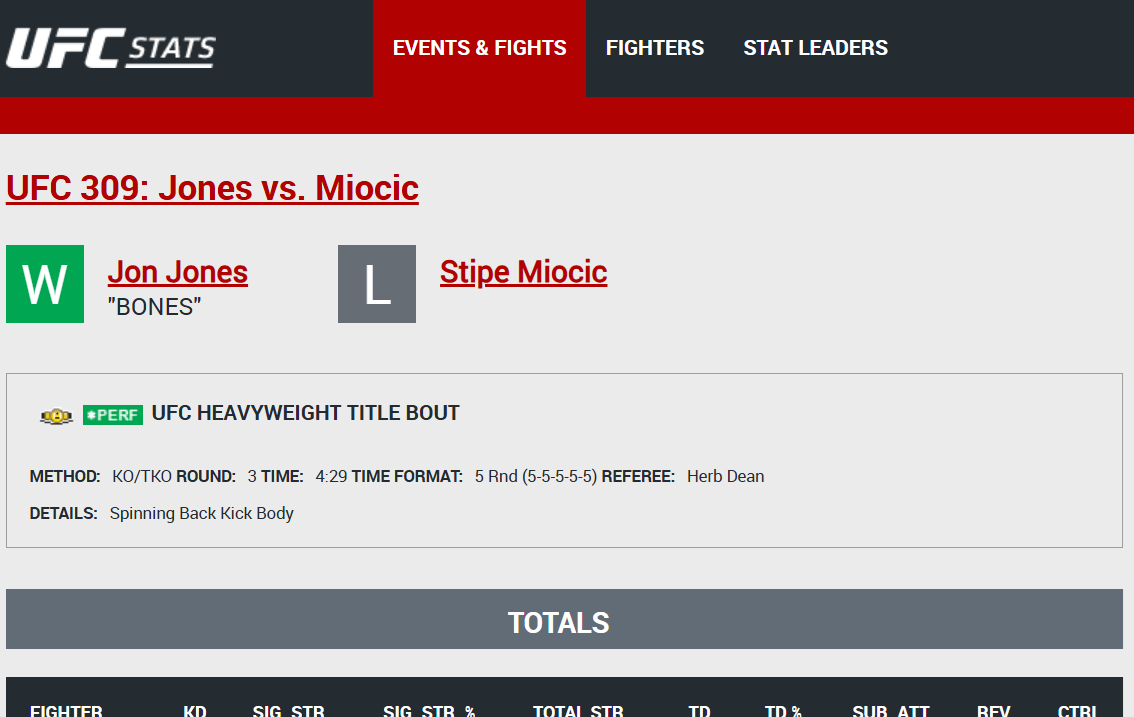
\includegraphics[width=0.95\linewidth]{figures/ufcstats1.png}
\end{subfigure}%
\begin{subfigure}{.5\linewidth}
  \centering
  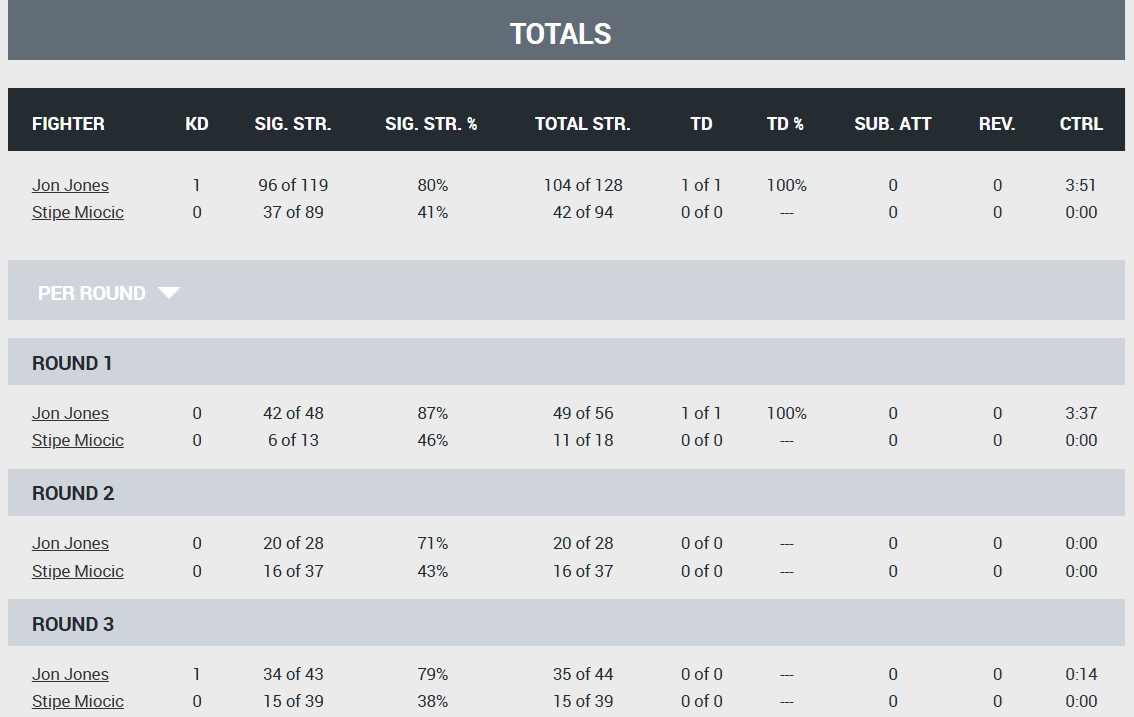
\includegraphics[width=0.95\linewidth]{figures/ufcstats2.png}
\end{subfigure}
% \begin{subfigure}{.3\linewidth}
%   \centering
%   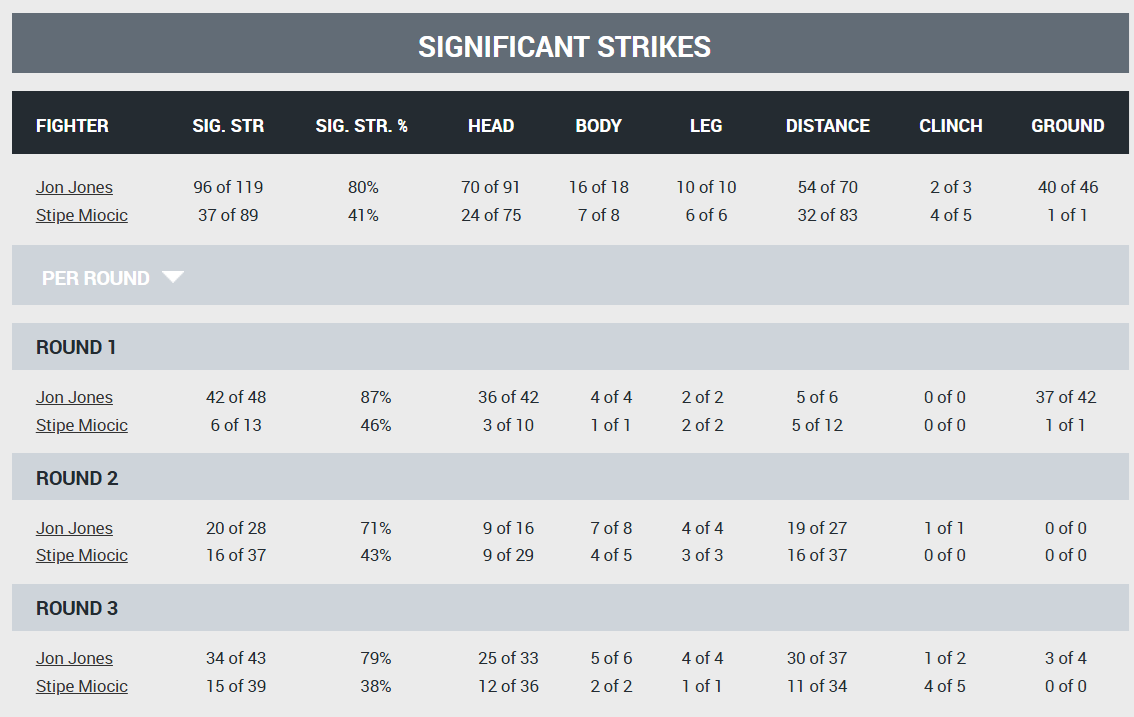
\includegraphics[width=0.95\linewidth]{figures/ufcstats3.png}
% \end{subfigure}
\caption{UFC Stats page for Jon Jones vs. Stipe Miocic}
\end{figure}


\subsubsection{ESPN}

ESPN provides comprehensive fight-level statistics similar to UFC Stats. While it lacks the round-by-round breakdown available on UFC Stats, ESPN compensates with more granular metrics, including striking statistics categorized by position (e.g., standing, clinch, ground) and targeted body regions (e.g., head, body, leg) simultaneously. UFC Stats on the other hand only includes these categorizations by position separately from targeted body regions. Additionally, the platform tracks advanced grappling metrics such as slams, guard passes, and positional advancements. 

\begin{figure}[htb]
    \centering
    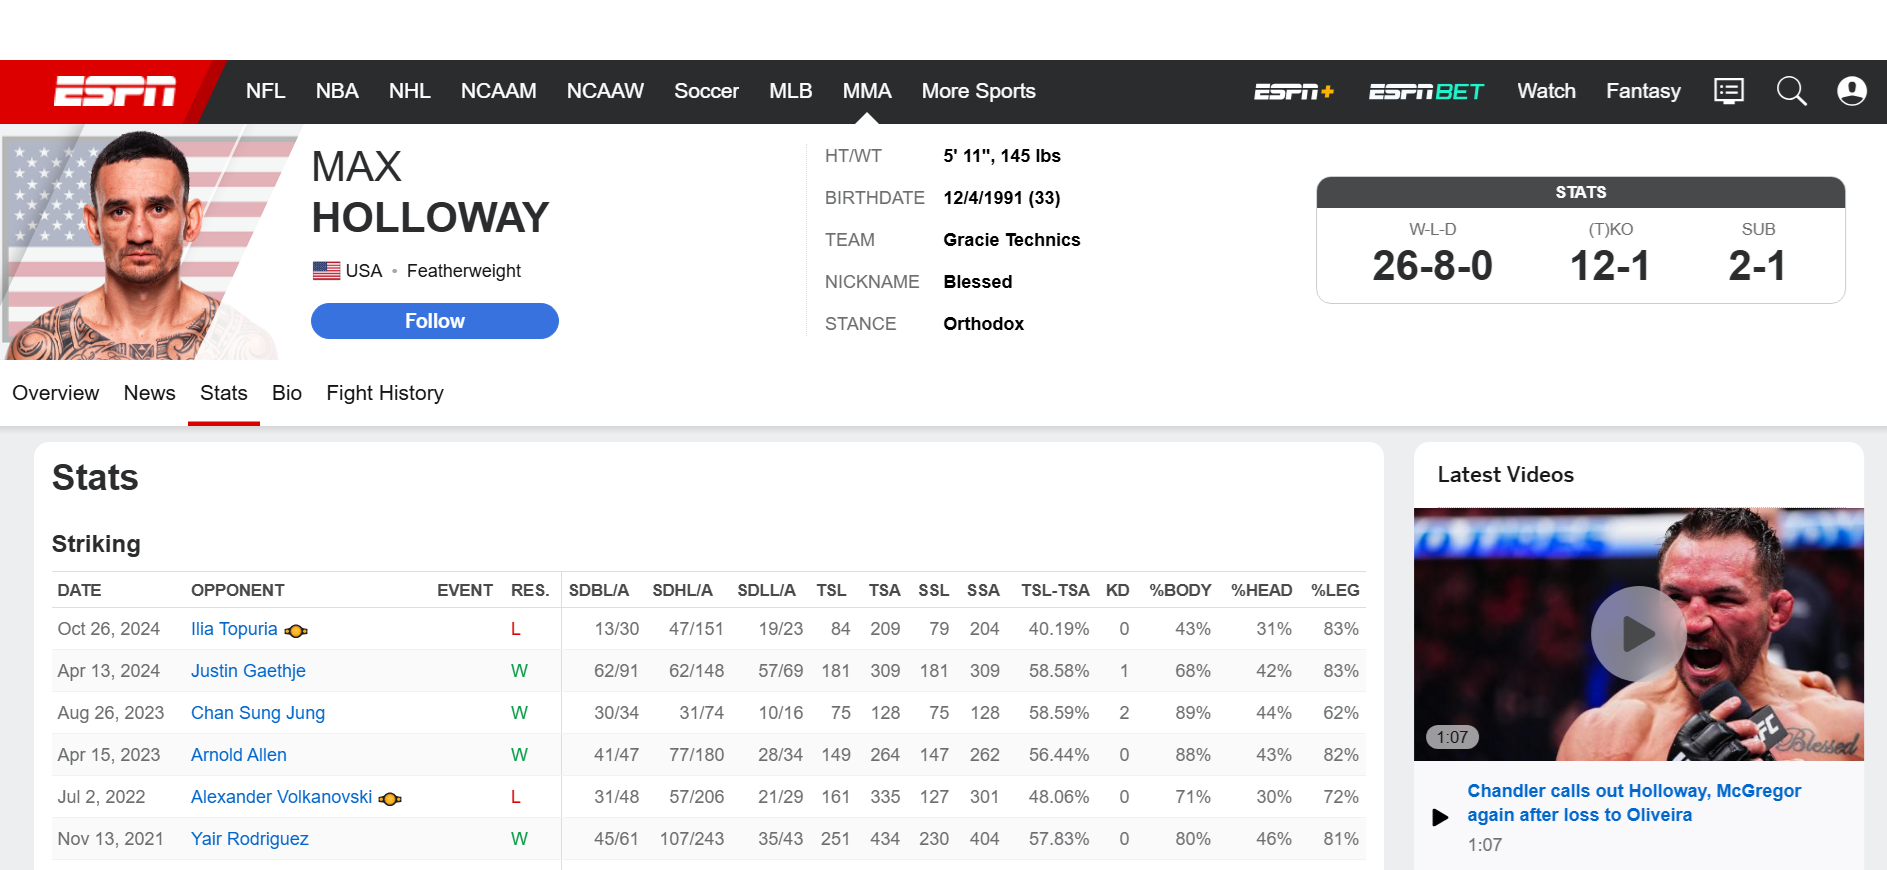
\includegraphics[width=0.6\linewidth]{figures/espn1.png}
    \caption{ESPN page for Max Holloway}
\end{figure}


\subsubsection{Wikipedia}

One of the key advantages of Wikipedia is its excellent tracking of the venues where both past and upcoming events have taken or will take place. To illustrate, venue names can change over time as new companies sponsor the same location, while the major physical attributes of the arena stay the same. For example, the Delta Center in Salt Lake City was previously called the Vivint Arena until 2023. Since Wikipedia redirects links associated with older venue names, we can essentially ``deduplicate'' the event locations. Moreover, almost all of the venue pages contain data concerning seating capacity as well as precise latitude and longitude coordinates that can be used to look up location elevations.

\begin{figure}[htb]
\centering
\begin{subfigure}{.5\linewidth}
  \centering
  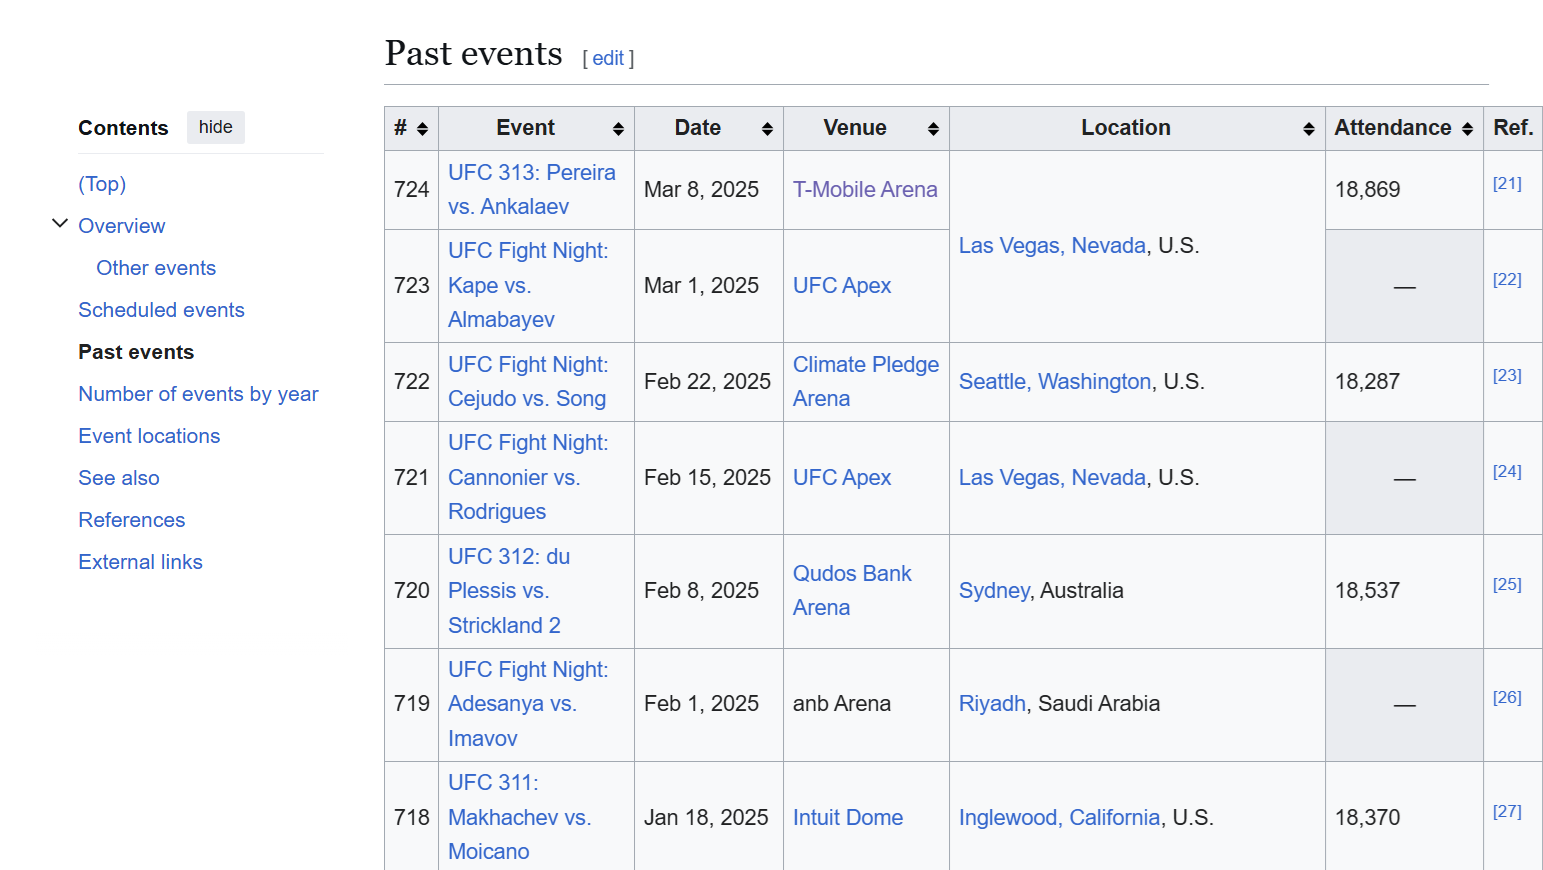
\includegraphics[width=0.95\linewidth]{figures/wikipedia1.png}
\end{subfigure}%
\begin{subfigure}{.5\linewidth}
  \centering
  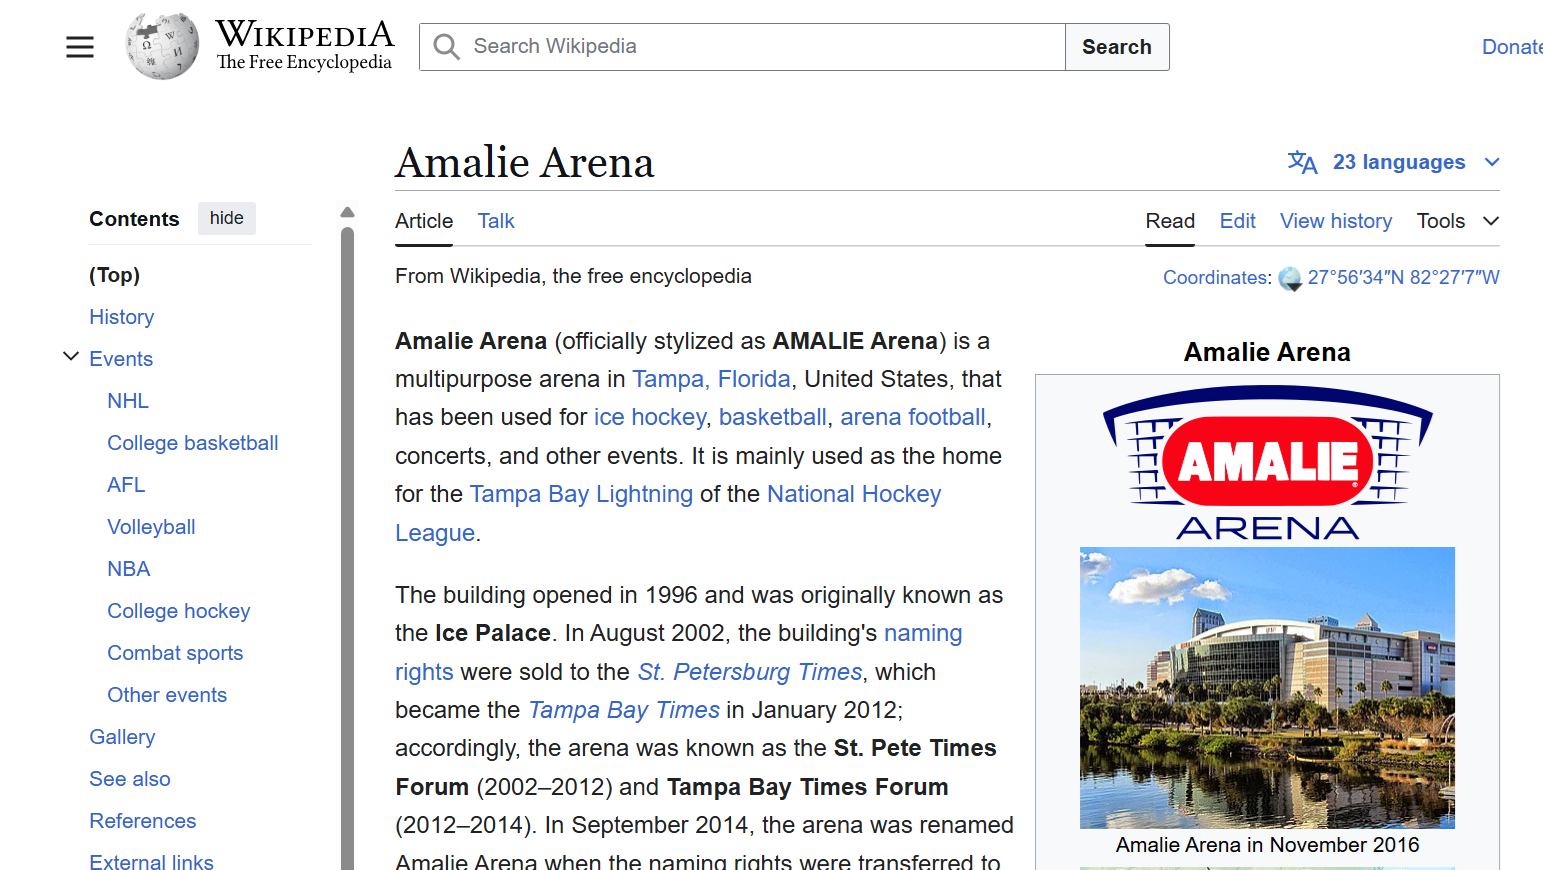
\includegraphics[width=0.95\linewidth]{figures/wikipedia2.png}
\end{subfigure}
\caption{Wikipedia pages for list of UFC events and Amalie Arena}
\end{figure}

\subsubsection{Sherdog}

Sherdog is one of the most established and widely recognized third-party sources for mixed martial arts data, serving as a comprehensive database for professional fighters and their fight histories. The platform provides detailed information on individual bouts, including dates, results, and methods of victory and cover virtually all promotions, from large ones like the UFC and the Professional Fighters League (PFL) to obscure regional agencies. This is valuable as most fighters in the UFC started their professional careers competing in smaller promotions and building their reputation before being signed, information that is omitted from sources like UFC Stats.

\begin{figure}[htb]
    \centering
    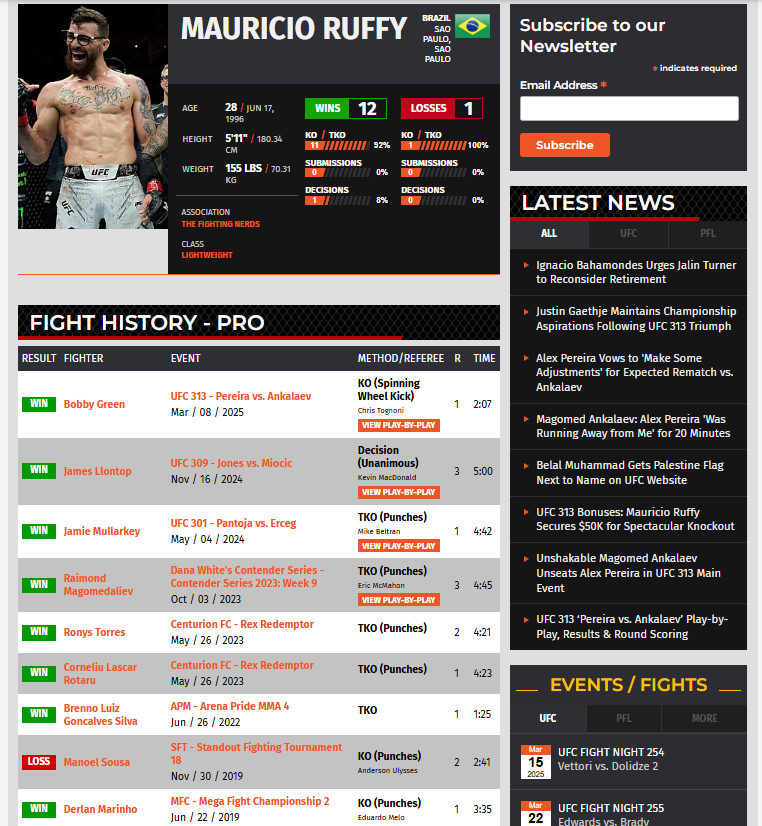
\includegraphics[width=0.55\linewidth]{figures/sherdog1.png}
    \caption{Sherdog page for Mauricio Ruffy}
\end{figure}


\subsubsection{Fight Matrix}

Fight Matrix is a third-party website that aggregates complete professional fight histories similar to Sherdog, but also maintains proprietary ranking and several Elo-like rating algorithms based on that data. The metrics generated by these algorithms are publicly available, automatically updated, and preserved historically, eliminating the need to create similar systems from scratch.

\begin{figure}[htb]
\centering
\captionsetup{justification=centering}
\begin{subfigure}{.5\linewidth}
  \centering
  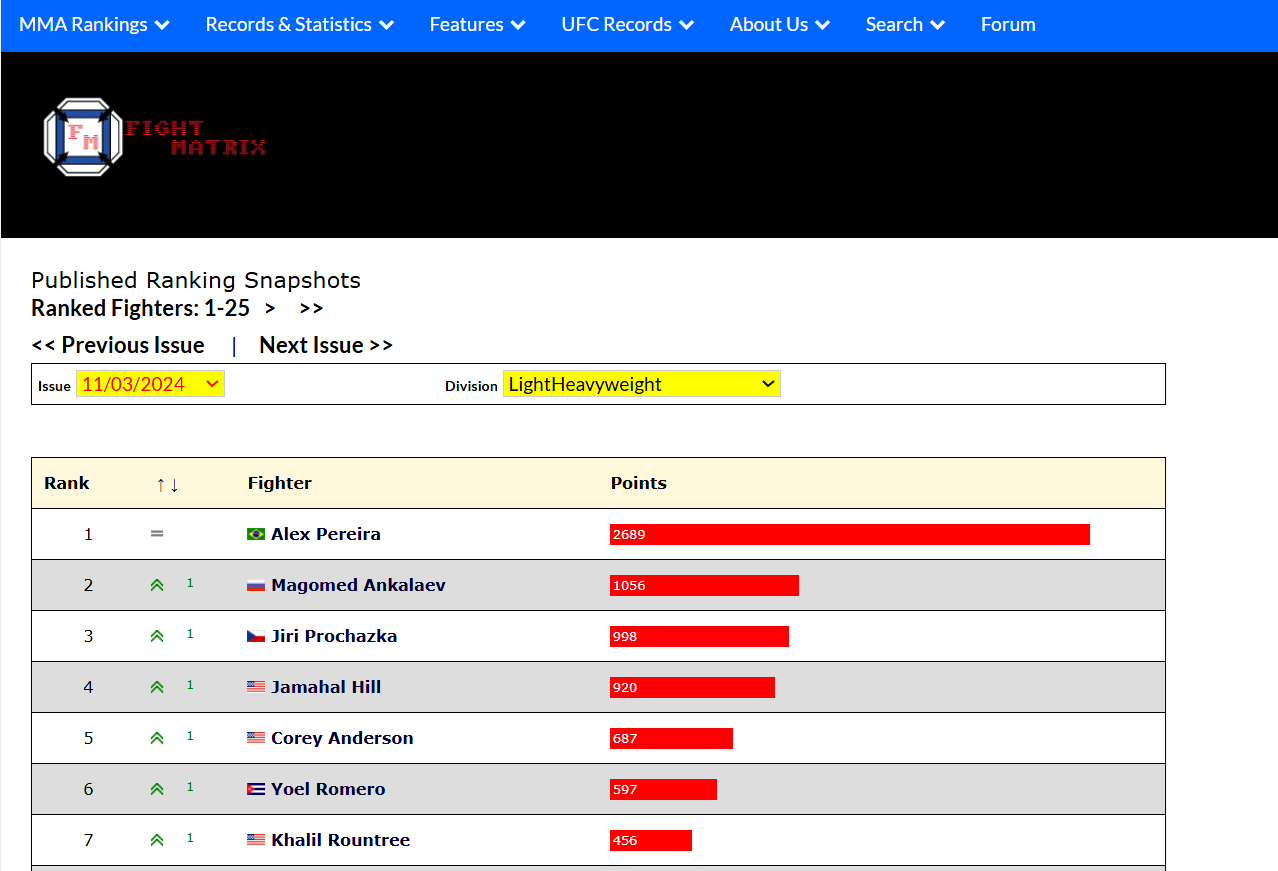
\includegraphics[width=0.95\linewidth]{figures/fightmatrix1.png}
\end{subfigure}%
\begin{subfigure}{.5\linewidth}
  \centering
  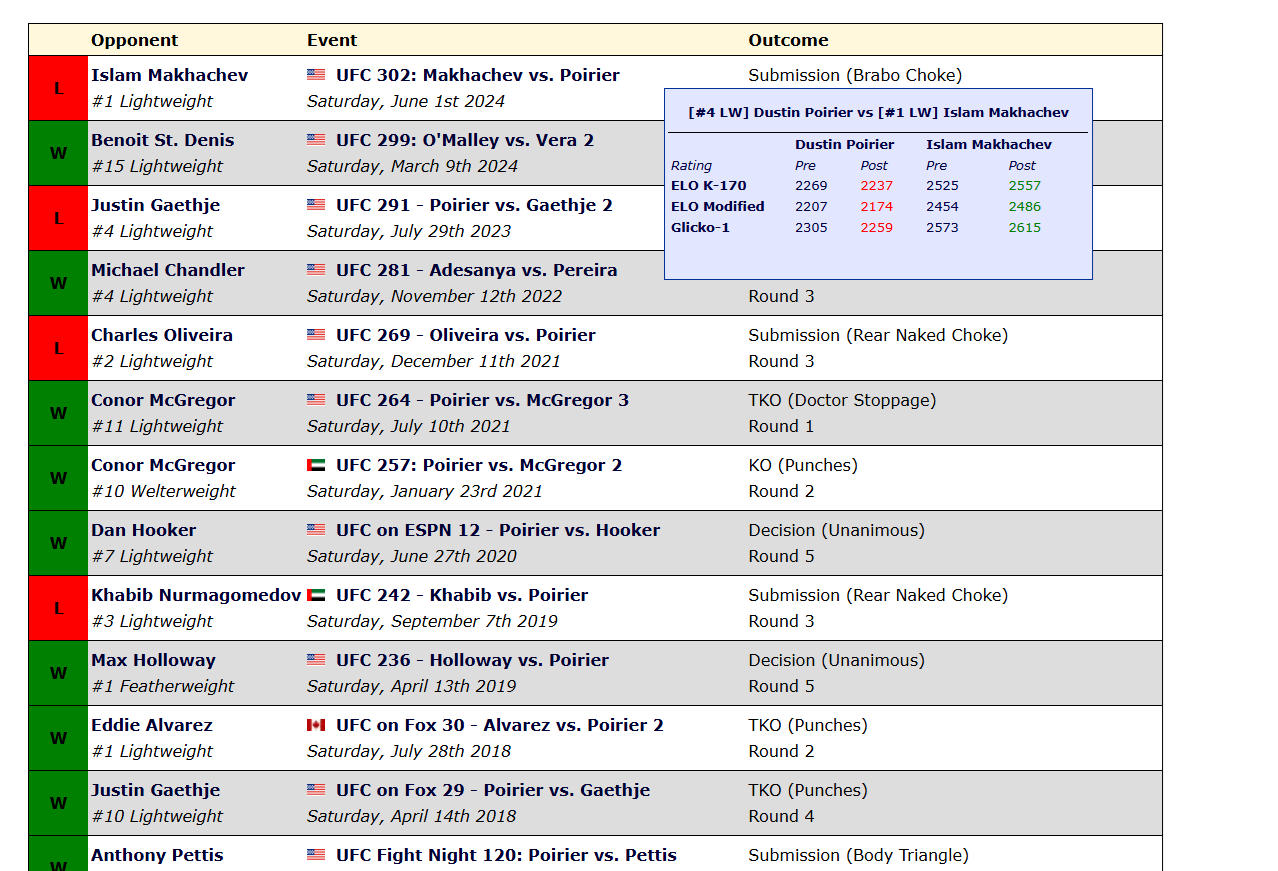
\includegraphics[width=0.95\linewidth]{figures/fightmatrix2.png}
\end{subfigure}
\caption{Fight Matrix pages for November 2024 Light Heavyweight division rankings and Dustin Poirier's fight history with Elo-like ratings}
\end{figure}


\subsubsection{Tapology}

Tapology is a community-driven platform that provides detailed metadata on fighters, events, and bouts. It tracks fighters' gym affiliations over time and records their exact weights at weigh-ins. The site also aggregates links to other platforms, including Sherdog, UFC Stats, and Best Fight Odds, for fighters, events, and bouts, simplifying the process of combining data from multiple sources.

\begin{figure}[htb]
\centering
\captionsetup{justification=centering}
\begin{subfigure}{.5\linewidth}
  \centering
  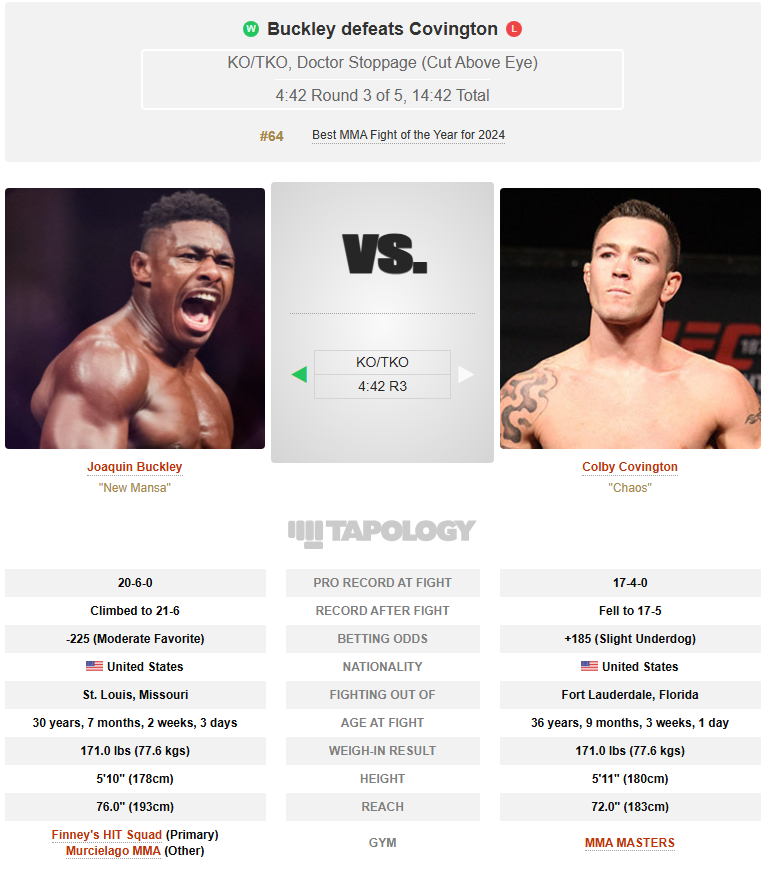
\includegraphics[width=0.7\linewidth]{figures/tapology1.png}
\end{subfigure}%
\begin{subfigure}{.5\linewidth}
  \centering
  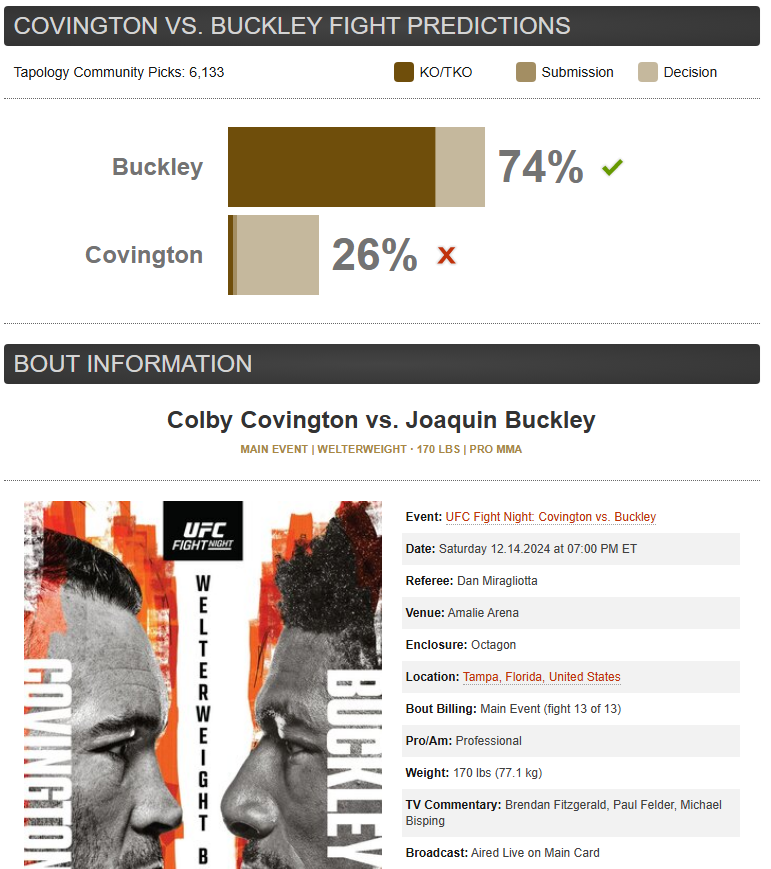
\includegraphics[width=0.7\linewidth]{figures/tapology2.png}
\end{subfigure}
\caption{Tapology page for Colby Covington vs. Joaquin Buckley}
\end{figure}


\subsubsection{MMA Decisions}

MMA Decisions specializes in granular round-by-round judge scoring data for fights that end in decisions across several promotions including the UFC. It also has information on point deductions, specifically the fighter penalized, the number of points, the round, and the reason; this could potentially be used to gauge a fighter's tendency to commit fouls or a more ``accurate'' reflection of how judges would have scored their performance based purely on striking and grappling. In addition, the site aggregates media scores from different outlets which reflect prominent community voices' opinions on how a fight should have been scored.

\begin{figure}[htb]
    \centering
    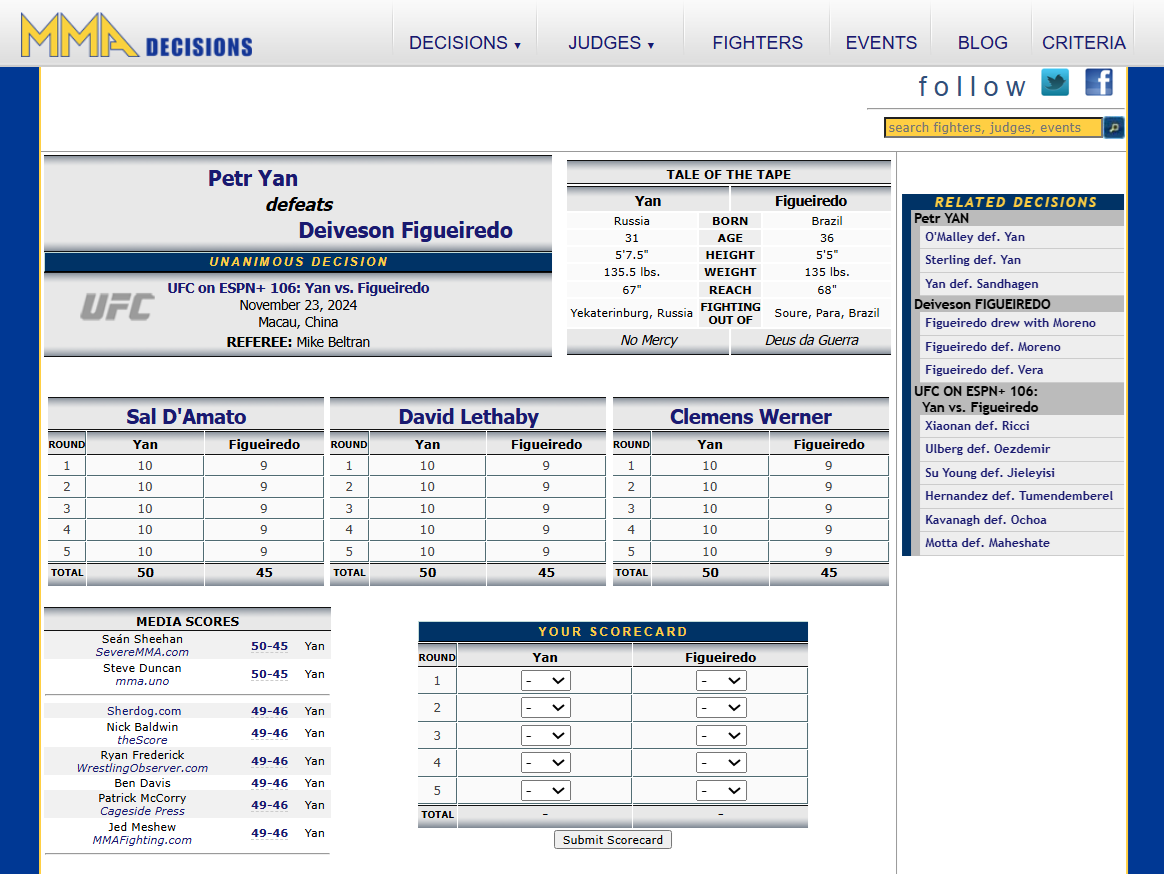
\includegraphics[width=0.5\linewidth]{figures/mmadecisions1.png}
    \caption{MMA Decisions page for Petr Yan vs. Deiveson Figueiredo}
\end{figure}


\subsubsection{Best Fight Odds}

Best Fight Odds is a prominent aggregator of betting odds for several MMA promotions, providing near real-time and historical odds from a variety of sportsbooks and offers including both moneyline and proposition bets. Odds are tracked over time from opening to closing lines, giving us granular time series data. The site is especially valuable due to how far the historical odds data goes back; in particular, the earliest UFC event with partial data is ``UFC 72: Victory" which took place in 2007.

\begin{figure}[htb]
    \centering
    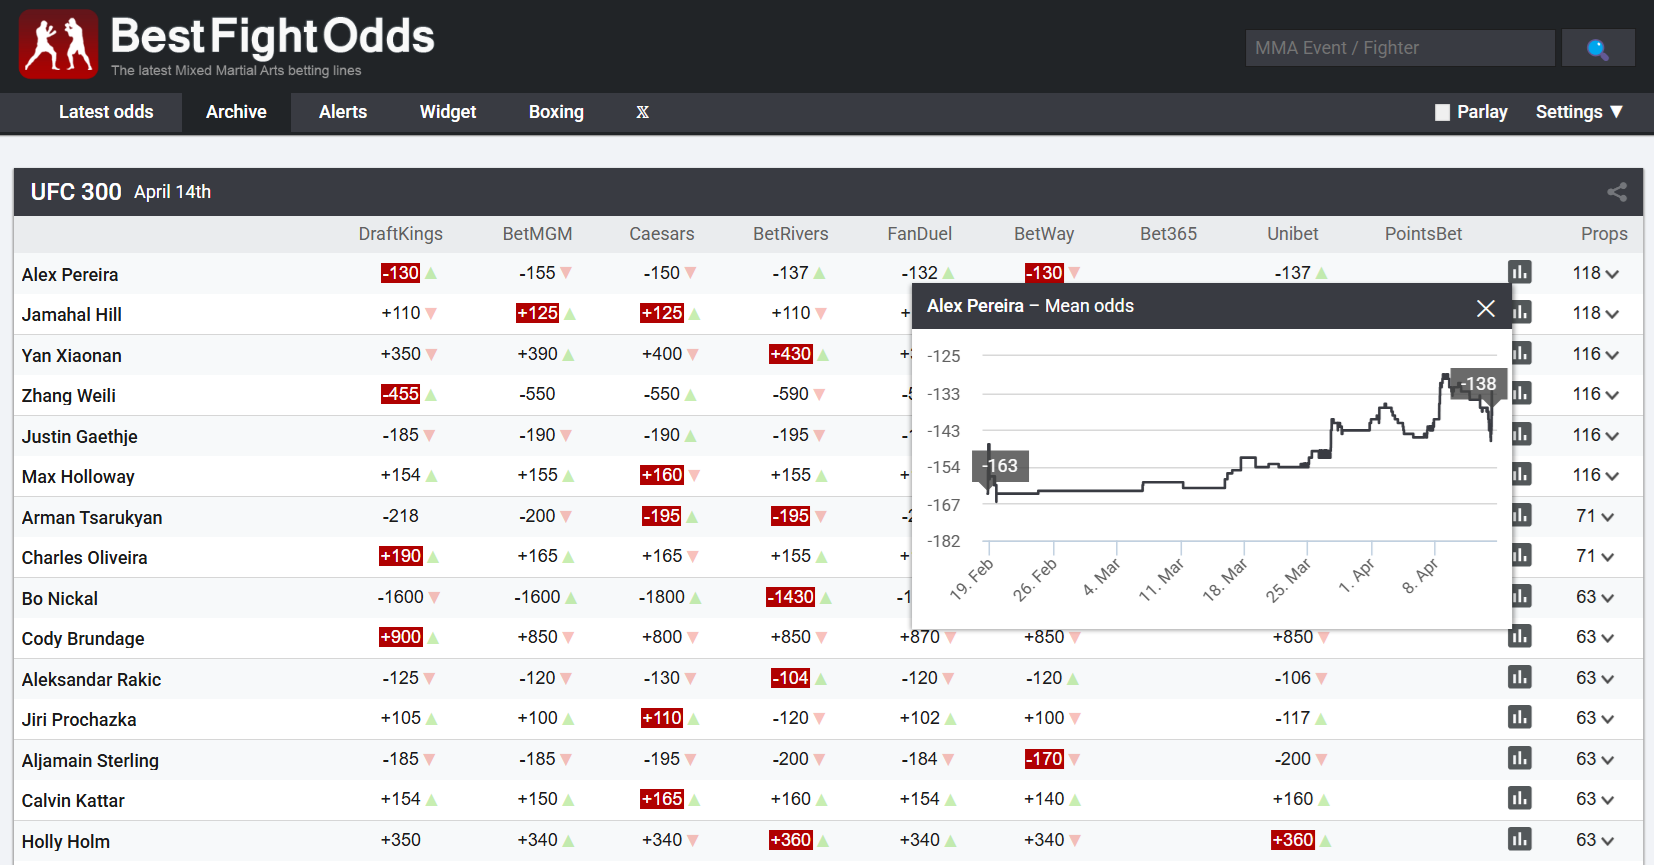
\includegraphics[width=0.5\linewidth]{figures/bestfightodds1.png}
    \caption{Best Fight Odds page for UFC 300}
\end{figure}


\subsubsection{FightOdds.io}

FightOdds.io also aggregates betting odds like Best Fight Odds but is significantly easier to obtain data from at the cost of having a shorter history. We specifically leverage the site to get historical opening and closing moneyline odds and average closing odds for expected outcomes (propositions), each consisting of well-structured and consistent metadata. The website essentially has perfect coverage for all bouts within the last several years.

\begin{figure}[htb]
\centering
\captionsetup{justification=centering}
\begin{subfigure}{.5\linewidth}
  \centering
  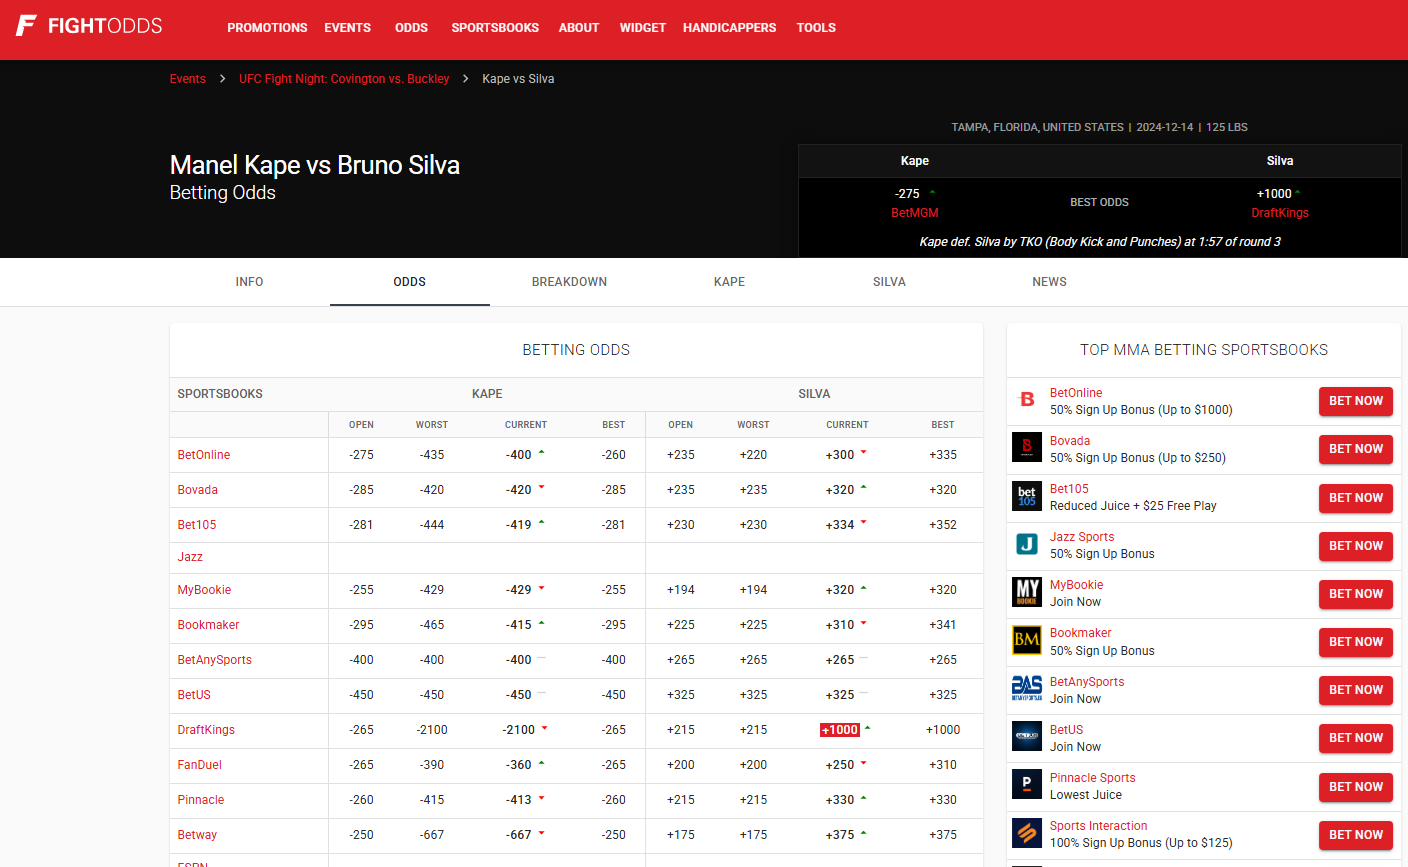
\includegraphics[width=0.8\linewidth]{figures/fightoddsio1.png}
\end{subfigure}%
\begin{subfigure}{.5\linewidth}
  \centering
  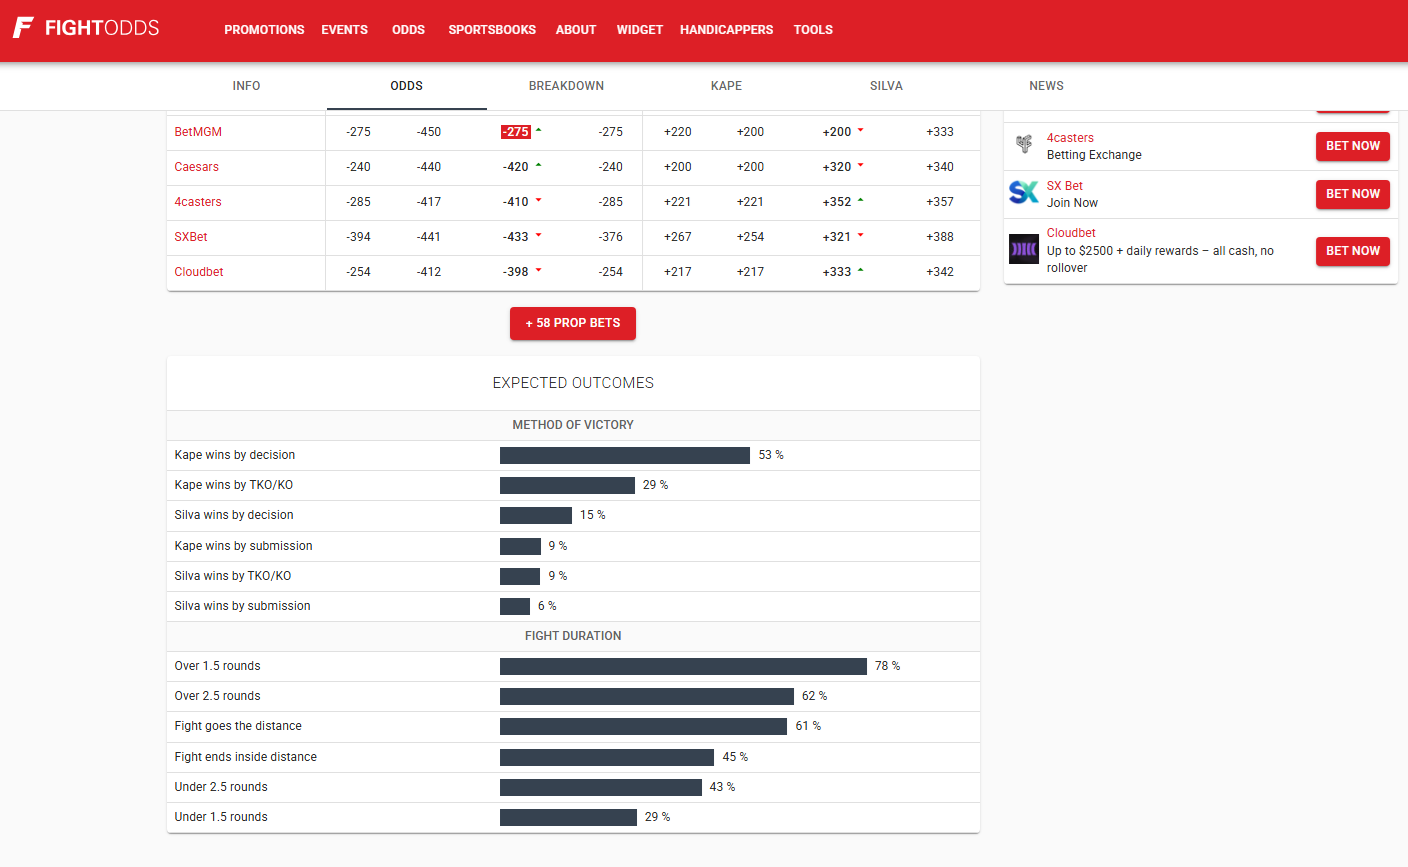
\includegraphics[width=0.8\linewidth]{figures/fightoddsio2.png}
\end{subfigure}
\caption{FightOdds.io page for Manel Kape vs Bruno Silva}
\end{figure}


\subsubsection{Bet MMA}

The main purpose of Bet MMA is to serve as a platform for sports handicapping, but the site also tracks fighters' moneyline odds history, data on fighters missing weight, and short notice fights.

\begin{figure}[htb]
    \centering
    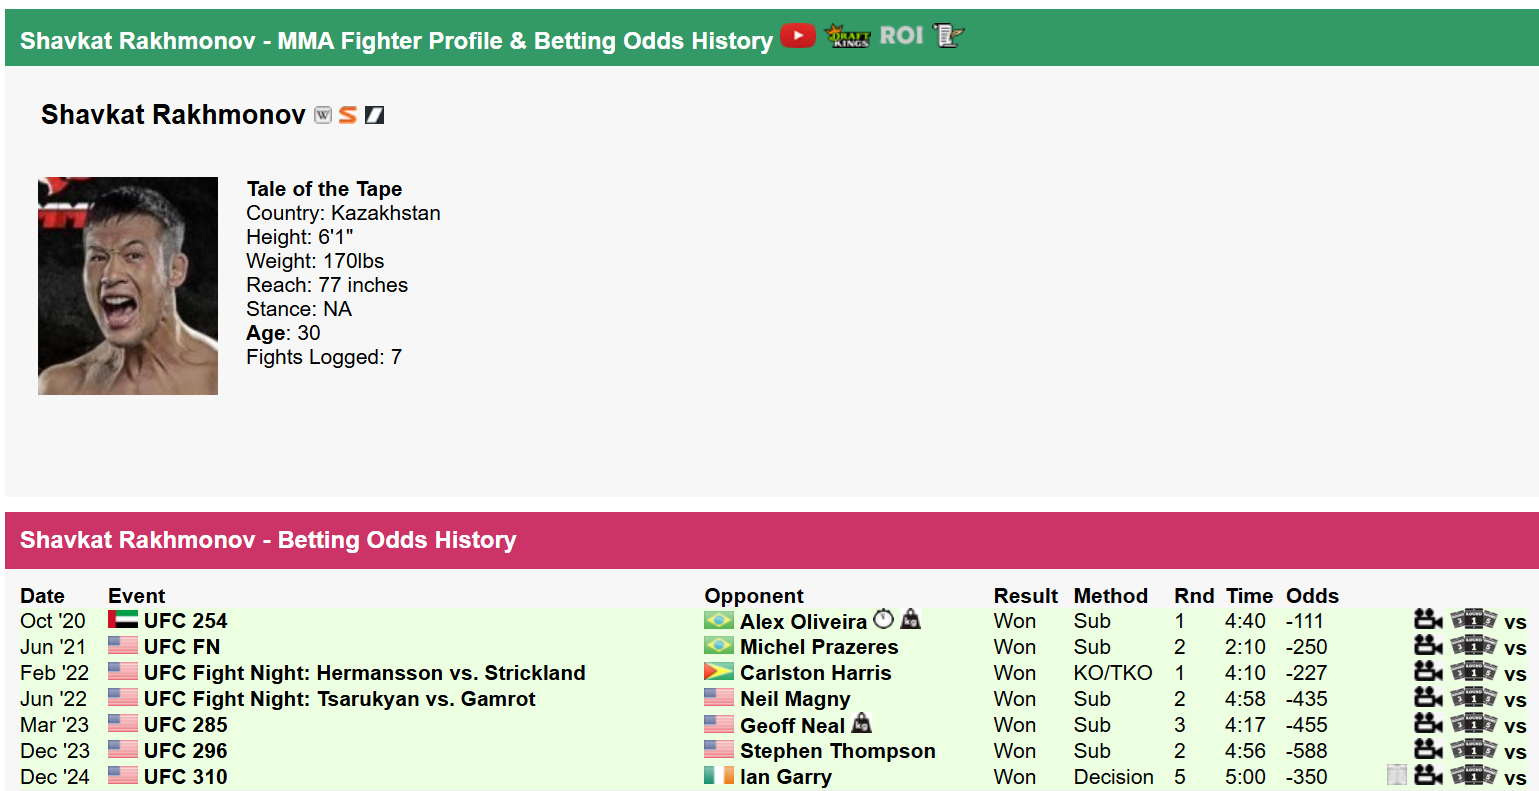
\includegraphics[width=0.5\linewidth]{figures/betmma1.png}
    \caption{Bet MMA page for Shavkat Rakhmonov}
\end{figure}


\subsection{Acquisition}

Data from Best Fight Odds was downloaded from an old GitHub repository created by user Ian Kotlier, last updated around five years ago as of writing. The Best Fight Odds website has recently undergone changes making it significantly more difficult to scrape, with historical time series data for odds made inaccessible for older events. Consequently, we elected to use data that has already been collected and made public to avoid unnecessary technical challenges. For all other data sources, we utilized the Scrapy framework to asynchronously crawl the respective websites with user agent rotation and extract structured information from the HTML. The ESPN and FightOdds.io websites, specifically, rely on hidden APIs which we were able to reverse engineer by inspecting each website's network activity; we used Scrapy to mimic API calls and parse the corresponding JSON responses while throttling crawl speeds to avoid rate limits. For all sources, we utilized user agent rotation with varying amounts of parellelism and random delays to prevent being blocked.

Crawling the Tapology website presented the most technical challenges due to its aggressive and unforgiving anti-scraping measures. Even with a slow enough crawl speed that mimicked the amount of time a real person would spend on a given page, the website would eventually block a user's IP address after some number of pages had been crawled. To circumvent this, we collected and stored all target links by page type and scraped in batches of 1000 pages before rotating IP addresses using a VPN provider.

\subsection{Cleaning}

When possible, data cleaning was directly integrated into the web scraping logic to handle common source-independent issues like ensuring consistent data types, replacing empty strings or malformed data with null values, and removing newline characters, leading, or trailing whitespace. All other data quality issues were handled manually or semi-manually on a case-by-case basis; while there are too many unique cases to discuss, the approach typically involved some combination of checking the corresponding web page for updates or hotfixes, cross-referencing other websites, and deducing the intended values behind human misinputs based on the proximity of keyboard keys. As a last resort, values suspected of being erroneous were replaced with null values to avoid making any strong assumptions.

One significant result of the cleaning procedure was an augmented set of fights that our models could be trained on. As mentioned earlier, fighters are assigned to either the red or blue corner in a given bout. This distinction was introduced to the UFC some time in the mid- to late 2000's, but the UFC Stats website, which is the only consistent source that tracks corner assignments, erroneously lists the winner of every fight before ``UFC Live: Vera vs. Jones" (March 21, 2010) as the red corner fighter. This is problematic because the red corner fighter wins approximately $58\%$ of the time and so considering all of those earlier bouts would taint the distribution of class labels. By cross-referencing pictures and corresponding captions of earlier events on Getty Images and in some cases digging through YouTube for old videotapes, it was possible to deduce fighters' corner assignments by looking at the color of the tape around their gloves. In the end, we were able to push the effective cutoff for model training back to ``UFC 83: Serra vs. St-Pierre 2" (April 19, 2008).


\subsection{Cross-Source ID Matching}

One of the key challenges in integrating fight data from multiple sources was matching event, fighter, and bout IDs across datasets. Since each data provider uses a different ID system, with some assigning integer-based IDs and others using string-based unique identifiers, it was necessary to develop a systematic approach for aligning these records. Our goal was to tie all information back to a central reference source, UFC Stats, ensuring that every event, fighter, and bout could be consistently linked across all datasets. Without a reliable ID matching process, data integration would be prone to inconsistencies, making feature engineering and downstream analysis unreliable.

Event ID matching was relatively straightforward, primarily because we scraped event date information when available and collected data in chronological order. Since fight promotions follow a sequential event structure, we could align events based on their order in each dataset. The only exceptions were a few edge cases in 2014 where two UFC events occurred on the same calendar date on two separate occasions. In these cases, we performed manual verification to ensure the correct mapping. Beyond these minor adjustments, event ID matching required little intervention beyond properly ordering the events in each source.

Matching fighter IDs was the most challenging aspect of the process due to frequent inconsistencies in names and metadata across sources. Fighters may be listed with different spellings, abbreviations, or missing components (e.g., middle names or initials). Additional inconsistencies stemmed from nicknames, date of birth mismatches, and occasional data entry errors. Because multiple fighters can share the exact same name, matching on name alone was unreliable. To resolve this, we followed an iterative approach:
\begin{enumerate}
    \item Extract unique fighter names from each source and attempt an exact or partial match.

    \item Identify cases of multiple matches and subset them out for further verification.

    \item Match using additional fighter attributes (e.g., date of birth, nickname, height) to disambiguate records.
\end{enumerate}
We repeated this process, gradually narrowing down unmatched cases until only a small set remained, which could then be manually verified.

Once event and fighter IDs were successfully matched, bout ID alignment was straightforward. Since each bout is almost always uniquely defined by two fighters and an event, we could generate a unified bout ID simply by performing a sequence of dataframe joins between the event and fighter mappings. This final step ensured that every fight had a unique identifier that was consistent across all sources.

Despite automating much of the matching process, some manual fixes were required for edge cases where metadata was missing or inconsistent across sources. One particularly helpful resource was Tapology, which often linked fighters, events, and bouts to external sources which we naturally had already scraped. Many of these external links contained the IDs of interest in the URLs, allowing us to directly extract and match IDs across datasets. In cases where discrepancies arose, these references were instrumental in confirming the correct mappings and ensuring consistency.


\subsection{Database Design}

The database was designed as a relational database using SQLite, with all data models and primary/foreign key relationships defined through SQLAlchemy. Once the database schema was established, cleaned CSV files were uploaded, ensuring that each table was properly structured while minimizing redundancy across tables by omitting columns when appropriate. Tables not only included source-specific information but also the results of the cross-source ID matching discussed above, allowing for table joins across sources and all engineered features to be tied back to the red/blue corner distinction tracked by UFC Stats. Due to the time-ordered nature and diversity of our data, a SQL database was chosen over handling CSVs with Pandas dataframes due to the amount of joining and window functions required for feature engineering. Further details on individual tables can be found in Appendix A.

\section{Feature Engineering}

Due to the number of potential feature ideas resulting from the richness of our dataset, we adopted a ``kitchen sink" approach to feature engineering, aiming to generate as many potentially relevant features as possible based on intuition and domain knowledge. While we conducted exploratory data analysis and created visualizations to validate some ideas, the majority of features were generated semi-systematically without extensive manual verification, as manually checking each one would have been prohibitively time-consuming. This approach allows us to capture a wide range of potential predictive signals, relying on subsequent feature selection and model evaluation to determine their actual usefulness later on. In total, we generated 3094 candidate features acknowledging ahead of time that a majority of these will be discarded in the modeling process.

To ensure that our features remained informative yet free of data leakage, we primarily relied on simple cumulative sums and averages when constructing base statistics from which our features are derived. Since our dataset is time-ordered, it was crucial to enforce a strict separation between past and future data for each fight. Every feature was designed to use only information that would have been available prior to the event, preventing any unintended leakage of future fight results into the model's training data. By maintaining this strict ordering, we mitigate the risk of inflated model performance due to information leakage, ensuring that our backtesting results accurately reflect realistic conditions.

Although the interpretability of our features was not a primary concern, we can loosely group them into three broad categories based on their scope and the type of information they encode. For each of the three feature groupings---event-level, bout-level, and fighter-level---we will provide an overview of the thought process behind their construction rather than detailing every single feature. Given the large number of engineered features, an exhaustive listing would be impractical. Instead, we will highlight key considerations in their design and provide a few representative examples from each category to illustrate the approach taken.

\subsection{Event-Level Features}

Event-level features refer to characteristics that are shared among all bouts in the same event rather than being specific to individual fighters or matchups. These features capture contextual factors that might influence fight outcomes due to environmental, logistical, or promotional considerations. Examples of such features include:
\begin{itemize}
    \item Venue elevation (meters): Higher elevations could impact fighter performance, particularly cardio endurance.

    \item Past average venue attendance: A proxy for event prestige and crowd intensity.

    \item Event type (PPV vs. Fight Night): Pay-per-view (PPV) or numbered events may have higher stakes and different matchmaking dynamics (such as fighter quality) than UFC Fight Night cards.

    \item Event country: The location of the event could impact judging tendencies, travel fatigue, or home-field advantage for fighters.
\end{itemize}
For categorical variables like event country, we avoid excessive one-hot encoding to prevent an explosion in feature space, which could lead to overfitting. Instead, we employ time-aware weight of evidence (WOE) encoding, computed as
$$\text{WOE}_c = \log\left( \frac{\sum_{i} \mathds{1}_{\{ Y_i = 1, C = c \}}}{\sum_{i} \mathds{1}_{\{ Y_i = 0, C = c \}}} \right)$$
for some categorical feature $C$ where the numerator and denominator represent the number of fights the red corner fighter won and lost in past events held when $C = c$ (e.g., a specific country). These proportions are computed only using fights from past events where that categorical level was present, ensuring that no future information leaks into feature construction. 

For first-time occurrences of a categorical variable (e.g., a country hosting a UFC event for the first time), we substitute the feature with the overall WOE of all past events. In the case of a true cold start (i.e., no past event data exists), we default to a neutral value of zero to avoid injecting arbitrary bias.

\subsection{Bout-Level Features}

Bout-level features capture characteristics specific to individual fights within an event. These features can be broadly categorized into structural properties of the bout and fighter matchup dynamics. Structural features include aspects like the scheduled number of rounds (e.g., standard 3-round fights versus 5-round main events/title fights) and the weight class in which the fight occurs. Meanwhile, matchup-based features focus on the interaction between the two fighters, such as fighting stance (e.g., orthodox vs. southpaw matchups).

To illustrate, if we plot win percentages by corner segmented by the red corner versus blue corner stance matchup, we see substantial variation across groups in Figure \ref{stance_matchups}. While some of this variation may be due to small sample sizes, especially in cases where all fights were won by fighters in one of the corners, a majority of these pairings occur frequently. 

\begin{figure}[!htb]
    \centering
    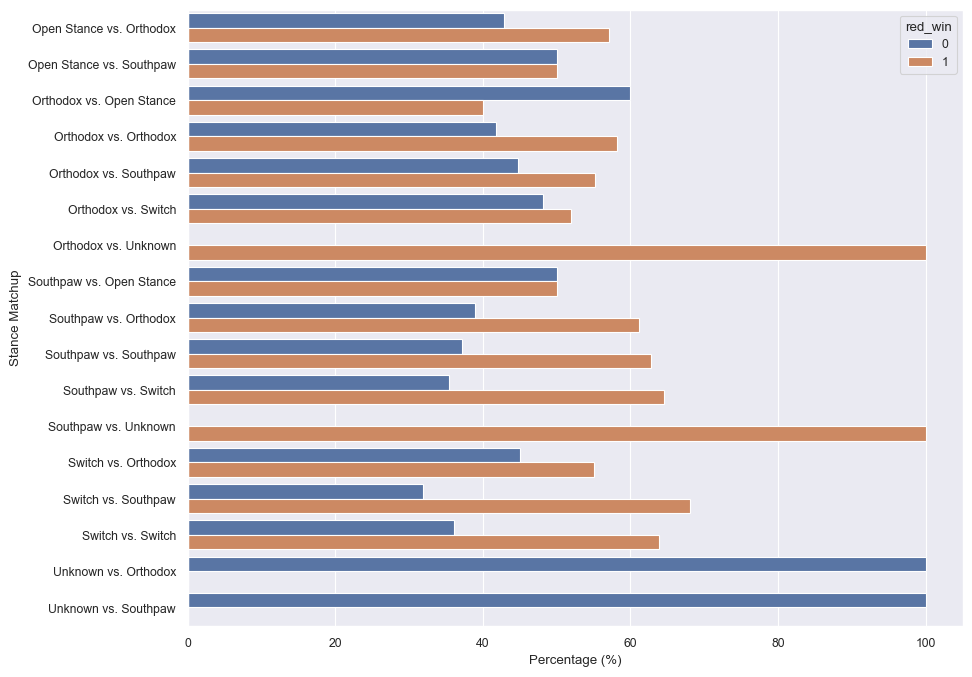
\includegraphics[width=\linewidth]{figures/stance_matchups.png}
    \caption{Win percentages of red corner and blue corner fighters by fighting stance matchup}
    \label{stance_matchups}
\end{figure}

We can repeat this for bout weight classes in Figure \ref{weight_classes}, where we again observe some differences in win percentages across groups, although much more subtle.

\begin{figure}[!htb]
    \centering
    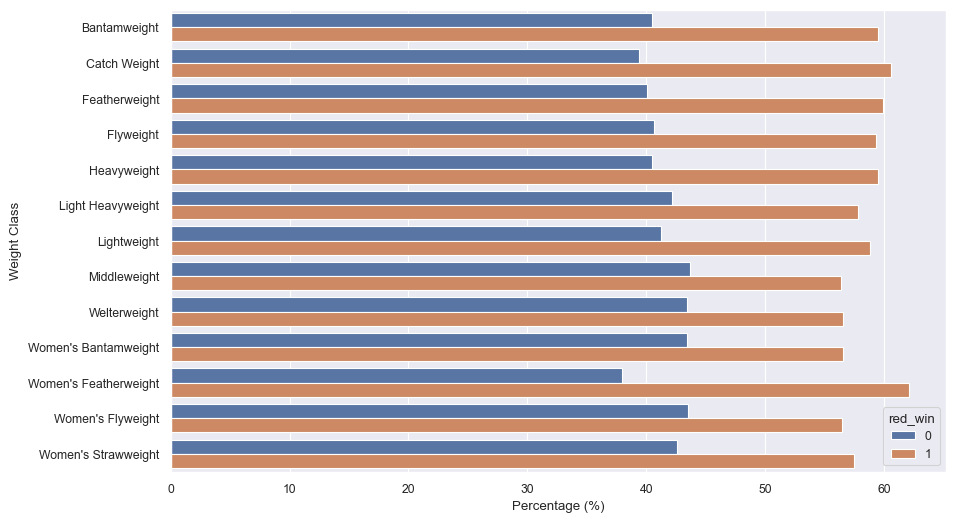
\includegraphics[width=\linewidth]{figures/weight_classes.png}
    \caption{Win percentages of red corner and blue corner fighters by weight class}
    \label{weight_classes}
\end{figure}

Categorical features like weight class and fighting style matchup were again encoded with weight of evidence encodings as described for event-level features.

\subsection{Fighter-Level Features}

Fighter-level features capture various aspects of a competitor’s background, physical attributes, and historical performance. These features encompass fighter physique (e.g., height, reach, age), fight history (e.g., UFC tenure, total fights, win/loss records), performance metrics (e.g., striking accuracy, takedowns landed per second), and rating/ranking trends over time to name a few. Given their depth and variety, fighter-level features were the most time-consuming to engineer and made up the bulk of the candidate features.

Our high-level approach ensured that each fighter’s statistics were calculated only using data that would have been available at the time of each fight, preventing any lookahead bias. Once these individual features were generated, we transformed them into comparative features by computing the difference between the red corner fighter’s value and the blue corner fighter’s corresponding value. This transformation had two key benefits:

\begin{enumerate}
    \item Feature Reduction: Instead of handling two separate sets of fighter statistics, we retained only a single difference-based feature for each metric, reducing dimensionality.

    \item Comparative Framing: The resulting features naturally aligned with how fights are assessed, emphasizing the relative advantage or disadvantage of one fighter over another rather than their standalone attributes.
\end{enumerate}
This comparative approach allowed us to encode meaningful matchup dynamics while maintaining a somewhat efficient feature set. If either fighter had missing data in their individual statistics before computing a difference, we set the difference to 0. This situation arose when a fighter was debuting in the UFC, particularly for striking and grappling stats sourced from UFC Stats, or had insufficient historical tracking. By setting the difference to zero, we effectively assume that both fighters are equivalent for that feature, which is likely suboptimal but serves as a simple and assumption-free approach to handling missing data, avoiding any bias in favor or against newcomers.

To construct the individual features before taking differences, we employed a multi-stage approach that progressively built more complex representations of a fighter's attributes and performance history.
\begin{enumerate}
    \item Base Features: We first derived fundamental features from static information such as date of birth, reach, height, and weigh-in results. These features required no aggregation or window functions.

    \item Expanding Sum/Average Features – Next, we introduced cumulative statistics that evolved over time, ensuring that all features reflected only historical data available prior to each fight. These included:
    \begin{itemize}
        \item Total fight time (seconds fought)

        \item Win rate at the time of each fight

        \item Cumulative significant strikes landed to the head per second

        \item Average change in Elo rating after each fight

        \item Expanding averages of base features (e.g., capturing a fighter’s average age at the time of their fights)
    \end{itemize}

    \item Opponent-Aware Features – To incorporate opponent quality, we performed a self-join by bout, allowing us to compute statistics such as:
    \begin{itemize}
        \item Average opponent’s features across past fights (e.g., average opponent height, reach, or win rate)

        \item Average historical differences between a fighter’s attributes and their past opponents’ attributes (e.g., average reach advantage, average striking accuracy differential)
    \end{itemize}
\end{enumerate}
For simplicity, we opted to use expanding windows rather than rolling windows when computing sums and averages. This means that each statistic was calculated using all available past fights rather than a fixed-length window of recent fights. Although rolling windows could have captured more recent trends, we avoided them to save on implementation time and to prevent further increasing the already prohibitively large number of candidate features.

We illustrate the class distribution for some of the more interpretable and easy-to-understand features that. In particular, we choose one comparative feature derived from an individual feature belonging to each of the three stages of complexity: difference in age in days, difference in average post-fight Gicko-1 rating change, and difference in the average difference in total time fought between fighters and their opponents during their full MMA careers. Although there is substantial overlap between the target classes for each of these features, there are clear directional trends that make sense intuitively. Based on the first histogram, the red corner fighter tends to win more often when they are younger than the blue corner fighter; we expect older fighters to be slower and more vulnerable due to years of accumulated damage. In the second histogram, it appears that the red corner fighter tends to win more often when their historical average change in Glicko-1 rating is greater than that of the blue corner fighter; since Glicko-1 attempts to capture skill while accounting for previous opponents' skills, it makes sense for fighters who on average fight tougher competition and are on the rise to win more often. Lastly, we can interpret the average difference in total time fought between fighters and their opponents during their full professional MMA careers as a proxy for how much more or less experienced a fighter's opponents have tended to be than the fighter in question. So, the third histogram supports the idea that fighters who have fought opponents who are relatively more experienced than them in the past tend to win more often.

\begin{figure}[!htb]
    \centering
    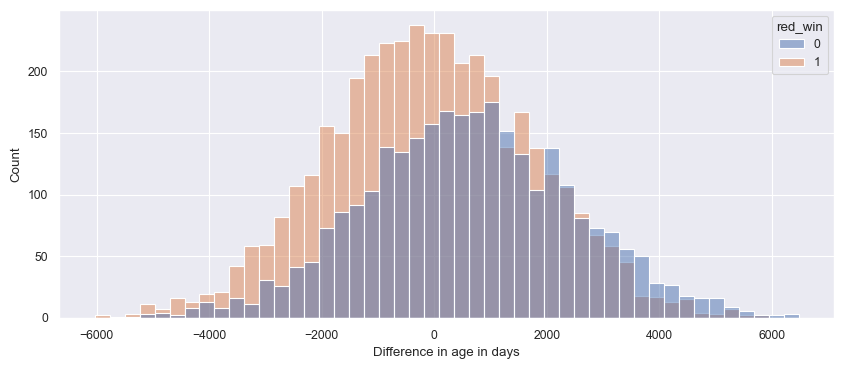
\includegraphics[width=\linewidth]{figures/age_days_diff.png}
    \caption{Histogram of difference in age in days by target}
\end{figure}

\begin{figure}[!htb]
    \centering
    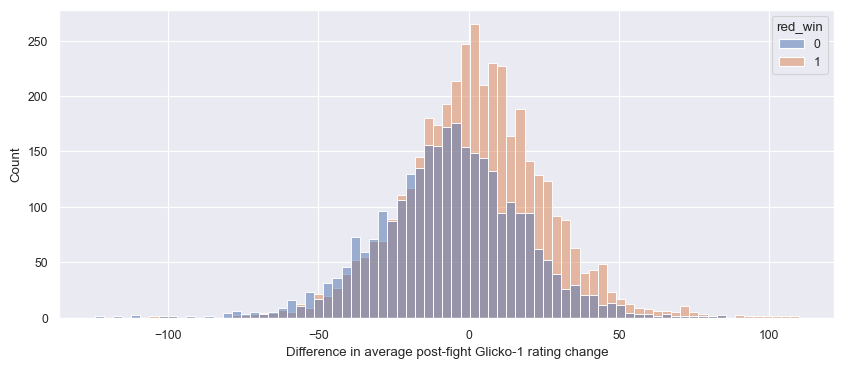
\includegraphics[width=\linewidth]{figures/glicko_1.png}
    \caption{Histogram of difference in average change in Glicko-1 rating by target}
\end{figure}

\begin{figure}[!htb]
    \centering
    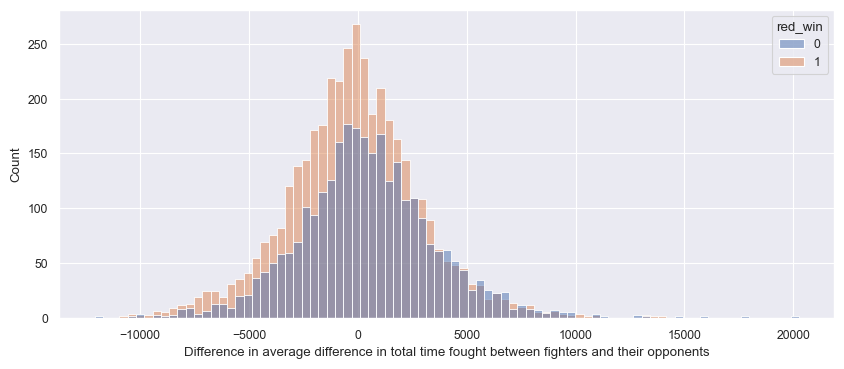
\includegraphics[width=\linewidth]{figures/super_convoluted_feature.png}
    \caption{Histogram of difference in average average difference in total time fought between fighters and their opponents by target}
\end{figure}


The most important feature, however, came from the betting market itself. We postulate that sportsbooks have information that we do not have access to or that they simply make more efficient use of the same data we have. To avoid situations where our models are missing out on crucial information, we can incorporate betting odds as a feature. In particular, we take the difference in fighters' average opening odds' implied probabilities across sportsbooks with the house edge removed. We choose to use the opening odds as these would reliably be available at any reasonable point in time in which we would place our bets (in contrast to closing odds, which by definition would never truly be available at the time of betting since we would no longer be able to place a wager). Moreover, they act as a sort of baseline guide that we can take advantage of and add differentiated value to with our other features. In Figure \ref{opening_implied}, it is clear that this offers the clearest separation between the classes.

\begin{figure}[!htb]
    \centering
    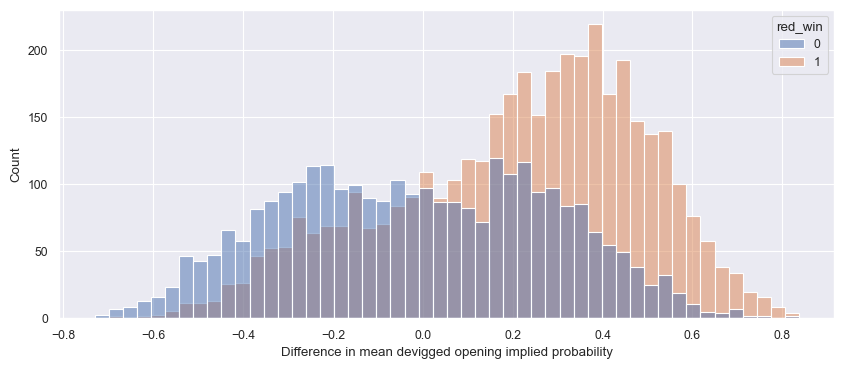
\includegraphics[width=\linewidth]{figures/opening_implied.png}
    \caption{Histogram of difference in mean devigged opening implied probability by target}
    \label{opening_implied}
\end{figure}


One potential concern of including the opening odds-based feature is that opening and closing odds tend to be correlated with each other. If our predicted probabilities mirror those implied by the betting odds too closely, we may struggle to identify betting opportunities where our estimates diverge from the market. At the same time, this should not be an issue if the rest of our features add predictive value and our models do not solely latch on to the opening odds-based feature, which can be diagnosed by examining feature importances. Opening lines may include traders' biases, but we try to mitigate this by averaging the odds across as many sportsbooks as possible. As an ablation study, we consider two variants of each proposed model pipeline discussed later, including and excluding this feature in the training data. 


\section{Modeling}

In this section, we detail the construction of the modeling pipelines used to estimate win probabilities for UFC bouts. Our approach consists of two broad pipeline variants:
\begin{enumerate}
    \item Feature selection $\longrightarrow$ base model

    \item Feature selection $\longrightarrow$ base model + probability calibration layer
\end{enumerate}
Additionally, we experiment with the inclusion and exclusion of the opening odds-derived feature as previously mentioned. The following subsections will break down each key component of these pipelines, including feature selection methods, model choices, and probability calibration techniques. We conclude this section with a discussion of hyperparameter tuning.

\subsection{Feature Selection}

Given the excessive number of candidate features and our belief apriori that many of these have little to no signal, we take a two-step feature selection approach to aggressively and efficiently reduce dimensionality.

First, we discard low-variance features using Scikit-learn's \texttt{VarianceThreshold} for a fixed threshold which operates on the fundamental statistical principle that features with low variance provide limited discriminative information for modeling. Mathematically, let $X \in \mathbb{R}^{n \times p}$ represent a training dataset with $n$ samples and $p$ features. For each feature $j \in {1, 2, ..., p}$, we calculate its variance $\text{Var}(X_j)$ across all samples. The selection criterion is then ``select feature $j$ if $\text{Var}(X_j) > \theta$." We choose $\theta = 0.05$, which roughly halves the number of candidate features, independent of the upper cutoff date of the training set.

Second, we rank all remaining features according to a scoring metric and retain the $k$ highest-scoring features. Formally, given $X \in \mathbb{R}^{n \times p}$ with $n$ samples and $p$ features, and a target vector $y \in \mathbb{R}^n$, we compute a score $S(X_j, y)$ for each feature $j \in {1, 2, ..., p}$. For our purposes, we choose $S(X_j, y)$ the mutual information between feature $X_j$ and the target $y$. Mutual information (MI) derives from information theory and quantifies the amount of information obtained about one random variable through observing another random variable. For a feature $X$ and target class $Y$, the mutual information is defined in terms of entropy as
$$I(X; Y) = H(X) - H(X \mid Y) = H(Y) - H(Y \mid X) = H(X) + H(Y) - H(X, Y)$$
where $H(X)$ is the entropy of $X$, $H(X|Y)$ is the conditional entropy of $X$ given $Y$, and $H(X,Y)$ is the joint entropy. Mutual information captures both linear and non-linear dependencies between variables, offering several advantages over correlation-based methods in that it (1) detects any functional relationship, not just linear associations, (2) is invariant to monotonic transformations of the variables, and (3) provides a natural measure of relevance in information-theoretic terms. For continuous variables, estimating mutual information becomes challenging as the true probability distributions are unknown. Various approaches exist, with Scikit-learn implementing nearest neighbors-based estimation method detailed in \citep{kraskov_2004}. We set the number of neighbors to $5$ for smoother estimates and let the number of features to retain, $k$, in \texttt{SelectKBest} be a tunable parameter.

Because our feature selection step relies on two univariate filter-based approaches that are model-agnostic, we ignore relationships between features and do not take into account which features work well together with which models, almost certainly leading to suboptimal feature subsets. However, this is not a large concern as our goals are exploratory in nature; if we sought maximum predictive performance and had more generous time and resource constraints, we would consider methods like recursive feature elimination with cross-validation or the Boruta algorithm for tree-based models. For the purposes of rapid experimentation and providing a preliminary analysis, these filtering methods serve as an adequate baseline.

\subsection{Base Models}

We now provide high-level overviews of the models used, outlining their fundamental principles, strengths, and weaknesses. We focus on logistic regression and gradient boosting with LightGBM, two models that differ significantly in complexity. Logistic regression offers interpretability and simplicity, while LightGBM captures nonlinear interactions and higher-order dependencies. Beyond theoretical contrasts, a key motivation for selecting these models is training speed---logistic regression allows for rapid baseline evaluation, while LightGBM efficiently handles complex patterns without excessive computation time. This balance enables fast experimentation and iterative model refinement.

\subsubsection{Logistic Regression}

Logistic regression is widely used to predict the probability of an event occurring by modeling the relationship between predictor variables and the log-odds of the outcome. It is popular as a benchmark due to its simplicity, but in turn offers advantages in training time and interpretation. The fundamental assumption of logistic regression is that the log-odds of the probability of success are linear in the covariates. Specifically, for a binary outcome $Y \in \{0, 1\}$ and feature vector $X = (x_1, x_2, \ldots, x_p)$, we assume
$$\log \left( \frac{P(Y = 1 \mid X)}{P(Y = 0 \mid X)} \right) = \beta_0 + \beta_1 x_1 + \beta_2 x_2 + \cdots + \beta_p x_p$$
Given a dataset $\left\{(X_i, Y_i) \right\}_{i=1}^{n}$, we estimate the coefficients $\beta$ by maximizing the log-likelihood function,
$$\mathcal{L}(\beta) = \sum_{i=1}^{n} \left[ Y_i \log P(Y_i \mid X_i) + (1 - Y_i) \log (1 - P(Y_i \mid X_i)) \right]$$
To prevent overfitting and improve generalization, we focus on $L_2$-penalized logistic regression such that for some regularization strength parameter $\lambda > 0$, we minimize the loss
$$J(\beta) = - \sum_{i=1}^{n} \left[ Y_i \log P(Y_i \mid X_i) + (1 - Y_i) \log (1 - P(Y_i \mid X_i)) \right] + \lambda \sum_{j=1}^{p} \beta_j^2$$
and leave $\lambda$ to be tuned later. All selected features from the previous pipeline step are centered and scaled to unit variance before training to ensure that features are penalized fairly.

\subsubsection{Gradient Boosting with LightGBM}

Gradient boosting is an ensemble learning method that sequentially combines weak learners, typically decision trees. Unlike bagging methods (e.g., random forests), where trees are trained independently in parallel, boosting builds trees in sequence, where each new tree corrects the mistakes of the previous one. For a dataset with input features $X$ and labels $y$, the model at iteration $t$ is updated as 
$$F_t (x) = F_{t - 1}(x) + \eta f_t(x)$$
where the learning rate $\eta$ controls how much each tree contributes. The trees are trained by minimizing a differentiable loss function $\mathcal{L}(y, F(x))$, which for our purposes is the log loss for binary classification,
$$\mathcal{L}(y, F(x)) = - \sum_{i=1}^{n} [y_i \log \hat{p}_i + (1 - y_i) \log (1 - \hat{p}_i)]$$
where $\hat{p}_i = \sigma(F(x_i))$ is the predicted probability after applying the sigmoid function. The key advantages of gradient boosting are that it optimizes errors iteratively and inherently capture non-linearities through feature interactions at tree splits. 

LightGBM is an optimized implementation of Gradient Boosting Decision Trees (GBDT), designed for efficiency and scalability. Unlike traditional boosting methods, LightGBM introduces two key innovations \citep{lightgbm_2017}:

\begin{enumerate}
    \item Gradient-based One-Side Sampling (GOSS): Instead of randomly sampling data, LightGBM retains instances with large gradients (high loss) and randomly downsamples instances with small gradients. This improves efficiency without significantly affecting accuracy, as high-gradient instances contribute more to information gain.

    \item Exclusive Feature Bundling (EFB):  Many datasets have sparse features (e.g., one-hot encoded categorical variables). LightGBM bundles mutually exclusive features into a single feature, reducing memory and computational cost.
\end{enumerate}
LightGBM also differs from standard gradient boosting in how it builds trees. Instead of evaluating every possible split, LightGBM bins continuous feature values into histograms, drastically speeding up training. Moreover, it grows trees leaf-wise rather than level-wise by following  leaves with the highest information gain, resulting in deeper, more efficient trees \citep{lightgbm_2017}.

\subsection{Probability Calibration with Venn-Abers Predictors}

In predictive modeling, particularly in applications such as betting, it is not enough for a model to simply rank outcomes correctly---it must also produce well-calibrated probabilities. A model is well-calibrated if the predicted probabilities accurately reflect the true likelihood of events. For example, if a model predicts a fighter has a 70\% chance of winning, we should be correct about 70\% of the time across all fights where we predict a 70\% chance. Poor calibration can lead to misleading confidence levels, resulting in suboptimal decision-making when placing bets. Even a model with strong predictive accuracy can be unprofitable if it systematically over- or underestimates probabilities, leading to inefficient bet sizing and unexpected risk exposure. Probability calibration allows us to post-process model outputs so that they better reflect estimates of probabilities.

In \citep{vovk_2014}, the authors introduce Venn predictors, a framework for probabilistic classification that provides validity guarantees regardless of the underlying data distribution at the cost of yielding multiprobability outputs, $(p_0, p_1)$, operating under the assumption of exchangeability or that the order of the data points does not contain additional information. We say that a random variable $P \in [0, 1]$ is perfectly calibrated if for $Y \in \{0, 1\}$, $\mathbb{E}[Y \mid P] = P$ almost surely. Then, one of the main properties of Venn predictors is that at least one of its two probability outputs is perfectly calibrated. A corollary to this is that $\mathbb{P}(Y = 1)$ is contained in the probability interval defined by the two probability outputs of Venn predictors in expectation (informally, we can say $p_0 \leq \mathbb{P}(Y = 1 \mid X) \leq p_1$). Venn-Abers predictors are a specialized subclass of Venn predictors designed for binary classification. They refine the probabilistic outputs by leveraging isotonic regression over the outputs of an underlying classifier, producing calibrated probability estimates while inheriting the core validity properties of Venn predictors.

In \citep{vovk_2015}, the authors discuss refinements to the original Venn-Abers framework designed to improve computational efficiency while preserving valid probability estimates, introducing the inductive Venn-Abers predictors (IVAP) and cross Venn-Abers predictors (CVAP) methods. The key idea behind IVAP is the division of data into a proper training set and a calibration set, allowing for the learning of a scoring function without repeatedly recalculating predictions for each test sample, which is implemented as:
\begin{enumerate}
    \item Partitioning: The dataset is split into two parts:
    \begin{itemize}
        \item A proper training set used to fit a traditional classifier.
        \item A calibration set used to compute probability corrections.
    \end{itemize}

    \item Scoring Function: A base classifier (e.g., SVM) produces scores for instances.

    \item Venn-Abers Calibration: The scores from the calibration set are used to fit two isotonic regression models, one for each class. These models map the classifier’s raw scores to calibrated probability estimates.

    \item Prediction: The learned calibration function is applied to new instances to produce valid probability estimates.
\end{enumerate}
IVAP maintains the validity property, meaning that the predicted probabilities are well-calibrated in expectation. However, a drawback is the dependency on the partitioning, which may introduce some variability in the results.

To mitigate the variability introduced by IVAP’s data split, the Cross Venn-Abers Predictor (CVAP) was proposed. CVAP employs cross-validation techniques to enhance stability while preserving the theoretical validity of the probability estimates with the following implementation:
\begin{enumerate}
    \item Cross-Validation Setup: The dataset is split into multiple folds, ensuring that each instance serves as both a training and calibration example in different runs.

    \item Multiple IVAP Models: Several IVAP models are trained using different folds. Each model yields probability outputs for unseen instances in its respective calibration set.

    \item Merging Predictions: The final probability estimates for test instances are obtained by averaging across multiple IVAP models, reducing variance and improving reliability.
\end{enumerate}
In particular, given the $p_0^1, p_0^2, \ldots p_0^k$ and $p_1^1, p_1^2, \ldots, p_1^k$ outputs from k-fold CVAP, for log loss we can obtain both a combined point estimate as
$$p = \frac{\text{GM}(\{p_0^1, p_0^2, \ldots p_0^k\})}{\text{GM}(\{1-p_0^1, 1-p_0^2, \ldots 1-p_0^k\}) + \text{GM}(\{p_1^1, p_1^2, \ldots p_1^k\})}$$
and a combined probability interval as
$$(p_0, p_1) = \left(1 - \text{GM}(\{1 - p_0^1, 1 - p_0^2, \ldots, 1 - p_0^k \}), \text{GM}(\{p_1^1, p_1^2, \ldots, p_1^k\})\right)$$
where $\text{GM}(\cdot)$ is the geometric mean. We will focus on the CVAP implementation for probability calibration purposes and are interested in both the point estimate and probability interval.

We adapted parts of the Python library \texttt{venn-abers} written by Ivan Petej \citep{petej_2024} and modified the cross Venn-Abers predictors (CVAP) implementation to better conform with the Scikit-learn API and not raise any warnings when used inside a \texttt{Pipeline} object. More importantly, we adjusted the \texttt{predict\_proba} method to directly output a pair of composite $p_0$ and $p_1$ values rather than a vector of $p_0$ and $p_1$ estimates for each fold. The current version of the library outputs the merged point estimate, but not a combined version of the probability interval at the time of writing.

\subsection{Summary of Model Pipelines}

In total, we consider 8 different model pipelines which we summarize in Table \ref{pipeline_table}. We include shorthand names for each pipeline to be referenced later for brevity.

\begin{table}[!htb]
\centering
\caption{Summary table of model pipelines}
\resizebox{\linewidth}{!}{%
\begin{tabular}{llll} 
\toprule
Base Model          & Opening odds? & Venn-Abers? & Shorthand                \\ 
\toprule
Logistic Regression & Yes           & No          & LR                       \\
Logistic Regression & No            & No          & LR + No odds             \\
Logistic Regression & Yes           & Yes         & VA + LR                  \\
Logistic Regression & No            & Yes         & VA + LR + No odds        \\
LightGBM            & Yes           & No          & LGBM                 \\
LightGBM            & No            & No          & LGBM + No odds       \\
LightGBM            & Yes           & Yes         & VA + LGBM            \\
LightGBM            & No            & Yes         & VA + LGBM + No odds  \\
\bottomrule
\end{tabular}
}
\label{pipeline_table}
\end{table}

We also include diagrams of each pipeline to make the order of components and their interactions more clear in Figure \ref{pipeline_diagrams}. When applicable, we will reference components by their Python class names.

\begin{figure}[!htb]
    \centering
    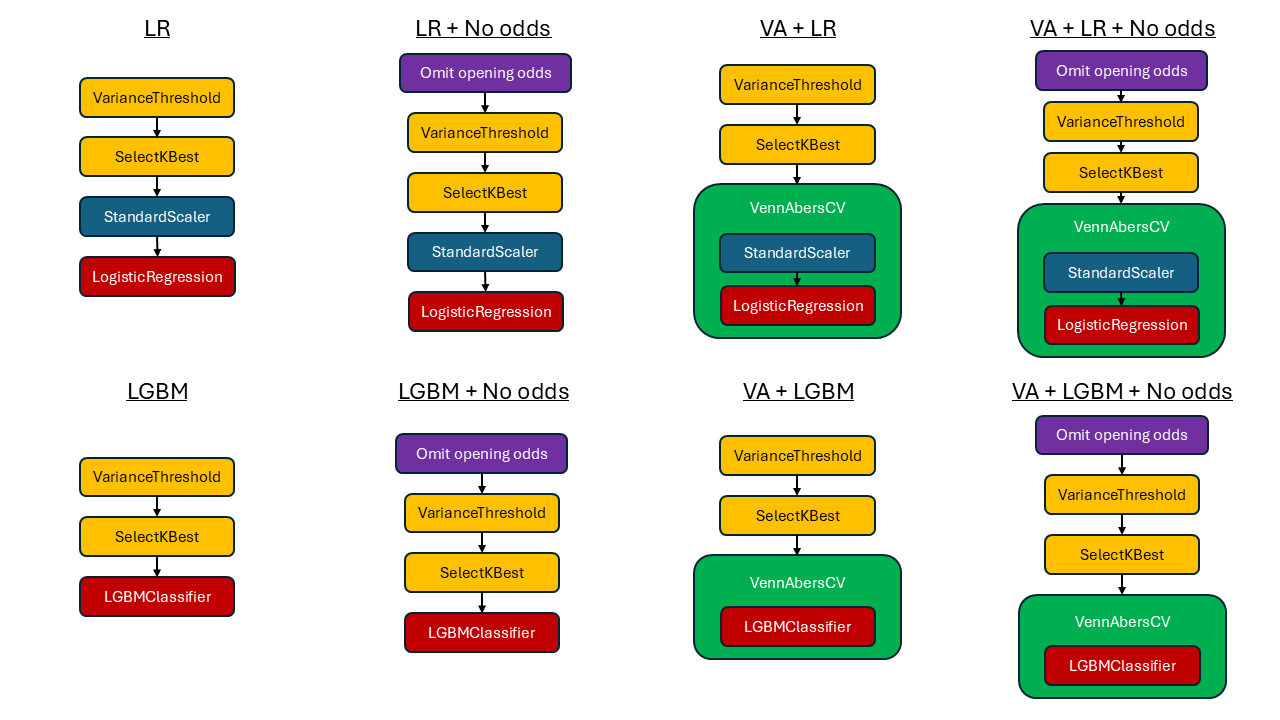
\includegraphics[width=\linewidth]{figures/pipeline_diagrams.png}
    \caption{Model pipeline diagrams}
    \label{pipeline_diagrams}
\end{figure}



\subsection{Hyperparameter Tuning}

We employed Optuna, an open-source hyperparameter optimization framework, to efficiently tune the parameters of our machine learning models. Optuna implements a Bayesian optimization approach called Tree-structured Parzen Estimator (TPE), which offers significant advantages over traditional hyperparameter tuning methods. Bayesian optimization fundamentally differs from conventional approaches by building a probabilistic model of the objective function and using it to select the most promising hyperparameters to evaluate next. Our decision to use Bayesian optimization rather than grid or random search was motivated by several key factors:
\begin{enumerate}
    \item Sample Efficiency: While grid search evaluates all possible combinations within discretized parameter ranges and random search samples randomly from parameter distributions, Bayesian methods use information from previous trials to inform subsequent parameter selections. This allows TPE to focus computational resources on promising regions of the parameter space, requiring fewer evaluations to find optimal configurations.

    \item Handling Complex Parameter Interactions: Unlike grid and random search, which treat parameters independently, Bayesian methods can capture complex interactions between hyperparameters.
\end{enumerate}
All optimization studies were run for a total of 200 trials with a fixed seed TPE sampler.

For cross-validation, we used a stratified k-fold cross-validation strategy with shuffling enabled and a fixed random seed for deterministic folds rather than a strictly time-based strategy. The primary justification for this choice is that our feature engineering process eliminates direct time dependencies since all features are computed only using past fight data, ensuring that no future data leaks into feature generation. We then proceed by treating each fight (row) as an independent instance. However, we acknowledge that this assumption is imperfect---there will naturally be folds where the model is trained on fights that occur after those in the validation set. This means that in some cases, a model may be learning from fighters who have already competed in later events within the training fold. While this may introduce a degree of data leakage in the strictest sense, we argue that this trade-off is acceptable given the constraints of our dataset. The primary drawback of a time series CV approach, where models are only trained on fights that occur strictly before those in the validation fold, is that it significantly reduces the number of effective training examples per fold. This is particularly problematic in small-to-moderate-sized datasets, where limiting training data in this way can lead to underfitting and unstable hyperparameter selection. Additionally, a time-based split risks overfitting to trends that are specific to a certain time period. By contrast, stratified k-fold CV ensures that each fold maintains the same distribution of fight outcomes, maximizing the efficiency of data use while still providing robust performance estimates. While time-aware validation is necessary for final model evaluation, using a stratified k-fold strategy for hyperparameter tuning enables us to identify generalizable patterns rather than trends specific to a single timeframe.

The computation of mutual information scores was consistently the most time-consuming and memory-intensive step in all of the modeling pipelines. This became an issue during hyperparameter tuning since a 10-fold cross-validation strategy meant that scores had to be computed 10 times for every Optuna trial. We introduced a simple optimization by setting the random seed of the mutual information scoring function to a fixed value and recognizing that across different trials, the scores used by \texttt{SelectKBest} should be exactly the same for a given fold (variance thresholding is already deterministic). By pre-computing and storing mutual information scores by fold and replacing the scoring function with a dummy function that performed a dictionary lookup based on the fold index, we drastically reduced the time required per trial and eliminated any ``out of memory" issues.

We tabulate each pipeline component/object's hyperparameters that we tune and the corresponding search spaces in Table \ref{hyperparams}. We also separately list any fixed parameters that were pre-specified and not tuned in Table \ref{fixed_params}.

\tiny 
\begin{table}[htb]
\centering
\caption{Tunable hyperparameters and search spaces}
\resizebox{\linewidth}{!}{%
\begin{tabular}{llllll} 
\toprule
Object                          & Parameter           & Description                          & Data Type & Lower Endpoint & Upper Endpoint  \\ 
\toprule
SelectKBest                     & k                   & Number of top features to select     & Integer   & 10             & 100             \\ 
\midrule
LogisticRegression              & C                   & Inverse of regularization strength   & Float     & 0.0001         & 100             \\ 
\midrule
\multirow{9}{*}{LGBMClassifier} & n\_estimators       & Number of boosted trees to fit       & Integer   & 100            & 1000            \\
                                & num\_leaves         & Maximum tree leaves per tree         & Integer   & 8              & 32              \\
                                & max\_depth          & Maximum tree depth                   & Integer   & 3              & 6               \\
                                & min\_child\_samples & Minimum data needed in a leaf        & Integer   & 100            & 300             \\
                                & subsample           & Subsample ratio of~training instance & Float     & 0.4            & 1               \\
                                & subsample\_freq     & Frequency of subsample               & Integer   & 0              & 10              \\
                                & colsample\_bytree   & Subsample ratio of columns           & Float     & 0.4            & 1               \\
                                & reg\_alpha          & L1 regularization term on weights    & Float     & 0.001          & 10              \\
                                & reg\_lambda         & L2 regularization term on weights    & Float     & 0.001          & 10              \\
\bottomrule
\end{tabular}
}
\label{hyperparams}
\end{table}
\normalsize

\tiny 
\begin{table}[htb]
\centering
\caption{Fixed parameters}
\resizebox{\linewidth}{!}{%
\begin{tabular}{lllll} 
\toprule
Object                                 & Parameter      & Description                                  & Data Type & Value                  \\ 
\toprule
\multirow{2}{*}{mutual\_info\_classif} & n\_neighbors   & Number of neighbors to use                   & Integer   & 5                      \\
                                       & random\_state  & Determines random number generation          & Integer   & 42                     \\ 
\midrule
SelectKBest                            & score\_func    & Function returning scores                    & Callable  & mutual\_info\_classif  \\ 
\midrule
\multirow{2}{*}{LogisticRegression}    & penalty        & Norm of penalty                              & String    & 'l2'                   \\
                                       & max\_iter      & Maximum number of iterations for solvers     & Integer   & 300                    \\ 
\midrule
\multirow{4}{*}{LGBMClassifier}        & objective      & Learning task                                & String    & 'binary'               \\
                                       & boosting\_type & Type of boosting                             & String    & 'gbdt'                 \\
                                       & learning\_rate & Boosting learning rate                       & Float     & 0.005                  \\
                                       & random\_state  & Random number seed                           & Integer   & 42                     \\ 
\midrule
\multirow{3}{*}{VennAbersCV}           & n\_splits      & Number of folds                              & Integer   & 10                     \\
                                       & random\_state  & Controls the shuffling applied               & Integer   & 492                    \\
                                       & shuffle        & Whether to shuffle the data before splitting & Boolean   & True                   \\
\bottomrule
\end{tabular}
}
\label{fixed_params}
\end{table}
\normalsize


\section{Bet Sizing}

Accurately modeling win probabilities is only part of a successful betting strategy---effectively translating predicted probabilities into optimal wager sizes is just as crucial, as improper bet sizing can lead to excessive risk, large drawdowns, or inefficient capital allocation. Even a bettor with only a slightly above break-even win rate can achieve significant long-term profits if they consistently place wagers with positive expected value and allocate capital efficiently. This is because profitability in betting is not just about how often one wins, but also the odds at which those wins occur and the fraction of capital risked on each bet. Proper bet sizing ensures that bankroll fluctuations are controlled, maximizing returns while mitigating the risk of ruin.

We use two such approaches: simultaneous Kelly gambling, which integrates with all 8 model pipelines, and a distributional robust variant, which integrates with the 4 model pipelines that include Venn-Abers calibration. In particular, we introduce a novel way of incorporating the Venn-Abers framework's multiprobability outputs into the distributional robust Kelly strategy for a polyhedron uncertainty set defined by linear inequalities and equalities.

\subsection{Simultaneous Kelly}

A common method for choosing wager sizes is to maximize the expected log growth rate of wealth, known as Kelly gambling. Using the notation in \citep{sun_2021}, suppose we have $n$ bets and $b \in S_n$ is the proportion of wealth allocated to each bet where $S_n$ is the probability simplex in $\mathbb{R}^n$ so that $b \geq 0$ and $1^T b = 1$. Let $r \in \mathbb{R}_{\geq 0}^{n}$ be a random vector with elements representing the returns on each bet such that if one had allocated a proportion $b$ of their total wealth $W$, their total return would be $r^T bW$ (note this is different from profit/loss). To ensure that we have the option to set aside money to not bet, we assign $r_n = 1$ which corresponds to $b = e_n$, the $n$-th standard basis vector, or not betting at all.

Now consider the case where only one of $K$ outcomes must occur that fully characterize the $n$ bets. If $r_1, r_2, \ldots, r_K$ are each of the $K$ return vectors and $\pi = (\pi_1, \pi_2, \ldots, \pi_K) \in S_K$ are the corresponding probabilities, we can define $R \in \mathbb{R}^{n \times K}$ to be the returns matrix with $r_1, r_2, \ldots, r_K$ as columns so that $R^T b$ is the wealth growth factor. Then, the expected log growth rate of wealth is
$$\begin{aligned}
    G_{\pi} (b) &= \mathbb{E}[\log(r^T b)] \\
                &= \pi^T \log(R^Tb)
\end{aligned}$$
where the logarithm is applied element-wise to the vector $R^T b$. Since $\pi$ is often unknown in reality, we replace it with an estimate $\hat{\pi}$ such as one derived from a probabilistic model. Finding the optimal bet allocation $b$ then becomes a problem of solving the following optimization formulation,
$$\begin{aligned}
    \max_{b} \quad & \hat{\pi}^T \log(R^Tb) \\
    \textrm{s.t.} \quad & 1^T b = 1 \\
                        & b \geq 0
\end{aligned}$$
which is convex and can be readily solved using CVXPY. Notice that $b = e_n$ will always result in an objective value of $0$ which corresponds to no change in wealth, so in expectation we will not lose money, assuming our probability estimates are accurate. This is rarely the case in practice, so to avoid financial ruin it is typical to multiply the wagers by some fraction $f$, $0 < f < 1$, so that we have allocation $fb$.

To connect this to betting on UFC fights, suppose there is an upcoming event with $m$ fights on the card ($10 \leq m \leq 15$ roughly for a typical event) that we would like to bet on and that we have already generated probability predictions $\hat{p}_r = (\hat{p}_{r, 1}, \ldots, \hat{p}_{r, m})$ and $\hat{p}_b = 1 - \hat{p}_r$ where $\hat{p}_{r,j}$ is our model's prediction for the red corner fighter's win probability for fight $j$. At the time of betting, suppose we have similarly indexed decimal betting odds $o_r = (o_{r_1}, \ldots, o_{r, m})$ and $o_b = (o_{b, 1}, \ldots, o_{b, m})$, such that $o_{r, j}$ represents the total dollar return (includes stake and profit) of betting one dollar on the red corner fighter in fight $j$ and winning the bet. We ignore the rare possibility of draws or no contests which would void any bets and automatically return corresponding wagers and assume that each fight must end in either the red corner or blue corner fighter winning. Then, there are $K = 2^m$ outcomes and $n = 2m + 1$ bets, one for each fighter and an additional risk-free ``no bet" asset corresponding to $e_{2m + 1}$. To illustrate, for $m = 3$ we construct $R$ and $\hat{\pi}$ to be
$$R = \begin{pmatrix}
    o_{r, 1} & o_{r, 1} & o_{r, 1} & o_{r, 1} & 0 & 0 & 0 & 0 \\
    0 & 0 & 0 & 0 & o_{b, 1} & o_{b, 1} & o_{b, 1} & o_{b, 1} \\
    o_{r, 2} & o_{r, 2} & 0 & 0 & o_{r, 2} & o_{r, 2} & 0 & 0 \\
    0 & 0 & o_{b, 2} & o_{b, 2} & 0 & 0 & o_{b, 2} & o_{b, 2} \\
    o_{r, 3} & 0 & o_{r, 3} & 0 & o_{r, 3} & 0 & o_{r, 3} & 0 \\
    0 & o_{b, 3} & 0 & o_{b, 3} & 0 & o_{b, 3} & 0 & o_{b, 3} \\ 
    1 & 1 & 1 & 1 & 1 & 1 & 1 & 1
\end{pmatrix}$$
and 
$$\hat{\pi} = \begin{pmatrix}
    \hat{p}_{r, 1} \cdot \hat{p}_{r, 2} \cdot \hat{p}_{r, 3} \\
    \hat{p}_{r, 1} \cdot \hat{p}_{r, 2} \cdot \hat{p}_{b, 3} \\
    \hat{p}_{r, 1} \cdot \hat{p}_{b, 2} \cdot \hat{p}_{r, 3} \\
    \hat{p}_{r, 1} \cdot \hat{p}_{b, 2} \cdot \hat{p}_{b, 3} \\
    \hat{p}_{b, 1} \cdot \hat{p}_{r, 2} \cdot \hat{p}_{r, 3} \\
    \hat{p}_{b, 1} \cdot \hat{p}_{r, 2} \cdot \hat{p}_{b, 3} \\
    \hat{p}_{b, 1} \cdot \hat{p}_{b, 2} \cdot \hat{p}_{r, 3} \\ 
    \hat{p}_{b, 1} \cdot \hat{p}_{b, 2} \cdot \hat{p}_{b, 3}
\end{pmatrix}$$
where the first column of $R$ corresponds to the betting returns in the outcome where every red corner fighter wins their fight and the first entry of $\hat{\pi}$ corresponds to our estimate for the probability of this occurring.

We take this more complicated ``simultaneous" approach rather than a sequential one to realistically simulate how one would bet using a system similar to ours due to fights being organized into events. One could imagine using our approach sometime between weigh-ins and the first fight of the event to capitalize on slightly more inefficient betting lines before the closing lines. In theory, one could bet sequentially but the short time window between fights would be a major inconvenience in addition to having to bet on the more efficient near-closing lines.


\subsection{Distributional Robust Kelly}

In \citep{sun_2021}, the authors introduce a distributional robust version of the Kelly strategy where the true distribution of outcome probabilities $\pi$ is unknown but we do know it belongs to some set of distributions $\Pi$. They then define the worst-case log growth rate of wealth as 
$$G_{\Pi}(b) = \inf_{\pi \in \Pi} G_{\pi} (b)$$
such that we now aim to find $b$ that maximizes $G_{\Pi}(b)$ instead.

One particular case the authors study is when $\Pi$ is defined by a finite set of linear inequalities and equalities,
$$\Pi = \{\pi \in S_K \mid A_0 \pi = d_0, A_1 \pi \leq d_1 \}$$
where $A_0 \in \mathbb{R}^{m_0 \times K}$, $d_0 \in \mathbb{R}^{m_0}$, $A_1 \in \mathbb{R}^{m_1 \times K}$, and $d_1 \in \mathbb{R}^{m_1}$. They derive that the problem then becomes
$$\begin{aligned}
    \max_{b, \mu, \lambda} \quad & \min(\log(R^T b) + A_0^T \mu + A_1^T \lambda) - d_0^T \mu - d_1^T \lambda\\
    \textrm{s.t.} \quad & 1^T b = 1 \\
                        & b \geq 0 \\
                        & \lambda \geq 0
\end{aligned}$$
with variables $b, \mu, \lambda$.

Now suppose we have a model that has been calibrated using Venn-Abers predictors (CVAP method in our case) and that we have access to the multiprobability outputs, $p_{0,j}$ and $p_{1, j}$, for each fight $j$ corresponding to the probability that the red corner fighter wins. Using the fact that $(1 - p_{1, j}, 1 - p_{0, j})$ is the corresponding interval for the probability that the blue corner fighter wins and the properties of Venn-Abers predictors, we can construct very crude estimates of lower and upper bounds $\hat{\pi}_l, \hat{\pi}_u$ for $\pi$ (in expectation) similar to how we constructed $\hat{\pi}$ in the original simultaneous Kelly problem. To illustrate, for the same $m = 3$ fights case as before, we define
$$\hat{\pi}_l = \begin{pmatrix}
    p_{0, 1} \cdot p_{0, 2} \cdot p_{0, 3} \\
    p_{0, 1} \cdot p_{0, 2} \cdot (1 - p_{1, 3}) \\
    p_{0, 1} \cdot (1 - p_{1, 2}) \cdot p_{0, 3} \\
    p_{0, 1} \cdot (1 - p_{1, 2}) \cdot (1 - p_{1, 3}) \\
    (1 - p_{1, 1}) \cdot p_{0, 2} \cdot p_{0, 3} \\
    (1 - p_{1, 1}) \cdot p_{0, 2} \cdot (1 - p_{1, 3}) \\
    (1 - p_{1, 1}) \cdot (1 - p_{1, 2}) \cdot p_{0, 3} \\
    (1 - p_{1, 1}) \cdot (1 - p_{1, 2}) \cdot (1 - p_{1, 3})
\end{pmatrix}$$
and 
$$\hat{\pi}_u = \begin{pmatrix}
    p_{1, 1} \cdot p_{1, 2} \cdot p_{1, 3} \\
    p_{1, 1} \cdot p_{1, 2} \cdot (1 - p_{0, 3}) \\
    p_{1, 1} \cdot (1 - p_{0, 2}) \cdot p_{1, 3} \\
    p_{1, 1} \cdot (1 - p_{0, 2}) \cdot (1 - p_{0, 3}) \\
    (1 - p_{0, 1}) \cdot p_{1, 2} \cdot p_{1, 3} \\
    (1 - p_{0, 1}) \cdot p_{1, 2} \cdot (1 - p_{0, 3}) \\
    (1 - p_{0, 1}) \cdot (1 - p_{0, 2}) \cdot p_{1, 3} \\
    (1 - p_{0, 1}) \cdot (1 - p_{0, 2}) \cdot (1 - p_{0, 3})
\end{pmatrix}$$
If we assume $\hat{\pi}_l \leq \pi \leq \hat{\pi}_h$, then we can equivalently write this in the form $A_1 \pi \leq d_1$ by letting
$$A_1 = \begin{pmatrix}
    -I \\
    I
\end{pmatrix}, \quad d_1 = \begin{pmatrix}
    -\hat{\pi}_l \\
    \hat{\pi}_u
\end{pmatrix}$$
where $I$ denotes the $2^m \times 2^m$ identity matrix. Since we do not have any equality constraints, our optimization formulation becomes
$$\begin{aligned}
    \max_{b, \lambda} \quad & \min(\log(R^T b) +  A_1^T \lambda)  - d_1^T \lambda\\
    \textrm{s.t.} \quad & 1^T b = 1 \\
                        & b \geq 0 \\
                        & \lambda \geq 0
\end{aligned}$$
with $R$ defined in the simultaneous Kelly problem and $A_1, d_1$ defined above.

\section{Backtesting}

Backtesting is a critical step in evaluating the effectiveness of our modeling and betting process by simulating how it would have performed on historical fight data. Since betting markets are inherently noisy and volatile, it is crucial to assess whether our model’s profitability is statistically robust or simply the result of random variance. A well-structured backtest allows us to quantify risk-adjusted returns, analyze performance stability over time, and ensure that the model’s edges are not the result of overfitting to past data.

Our approach to backtesting is far more rigorous and robust than previous works, which often suffered from limited sample sizes, overfitting, and insufficient safeguards to ensure that backtest conditions accurately mirrored reality. We address these shortcomings by:
\begin{enumerate}
    \item Using a backtest period spanning multiple years, ensuring that results are not skewed by short-term market inefficiencies and that a large number of bets are placed.

    \item Mirroring real-world betting conditions by having complete and accurate betting odds data as well as including all fights such as those that ended in draws, no contests, bad judging, or disqualifications to simulate voided bets and unexpected losses or gains.

    \item Emulating how one would realistically ingest incoming fight results into a regular refitting and complete retraining/retuning schedule for our models.
\end{enumerate}
By structuring our backtest to closely replicate authentic conditions, we provide a far more reliable assessment of our strategy’s viability and potential profitability.

\subsection{Setup Details}

We reserve a backtest period of 8 years consisting of all 3960 fights in the UFC between January 1, 2017 and December 31, 2024 across 331 events. This is necessary because of how infrequently fights take place compared to other sports and the fact that not every fight will be a profitable betting opportunity. As a result, we need to aim for a large sample size of bets while taking into account that this number will likely be a small fraction of the total number of fights.

We used the closing odds provided by offshore online sportsbook Bovada, as it had the most complete betting odds data during this period, and substituted closing odds from Pinnacle or BetOnline when unavailable. We do this despite the fact that, in practice, we would place bets sometime between the weigh-ins and the first fight of an event (typically 24 hours before). The primary justification for this choice is that closing odds incorporate the most information and are generally regarded as the most efficient market price, meaning they best reflect the true probabilities of fight outcomes. If our system can consistently generate profits against these sharper lines, it suggests a strong underlying edge. In reality, when we would actually be placing bets, we would be going against softer, less-efficient odds, which means our true expected profitability would likely be higher than what the backtest suggests. By using the closing line as our benchmark, we are effectively holding our system to the highest possible standard---if it can outperform this, it should theoretically perform at least as well in a more realistic setting.

We first generated predictions for each fight in the following manner for every model pipeline:
\begin{enumerate}
    \item Tune hyperparameters on fights between April 19, 2008 and December 31, 2016 with draws and no contests omitted and refit the model pipeline on all of these fights with the best parameters.

    \item Predict win probabilities (and the intervals for pipelines with Venn-Abers calibration) for the first event in 2017 and store results.

    \item Subset the fights from this event that did not end in a draw or no contest and concatenate to the training data. Refit the model pipeline with the same hyperparameters from step 1. Repeat steps 2 and 3 for subsequent events until the last event in 2017.

    \item Go back to step 1 and retune hyperparameters on data up to December 31, 2017 and repeat steps 1-4 to the end of 2024 until predictions have been generated for all fights in the backtest period.
\end{enumerate}
Plots of the optimization histories as well as the best hyperparameters for each model pipeline and training data cutoff year can be found in Appendices B and C.

Then, using these predictions and the closing odds, we iterate through events sequentially and simulate placing bets for the specified model pipeline and betting strategy, keeping track of the bankroll after each event, the cumulative number of bets placed, the total amount of money wagered, and the total amount of money returned. We assume an initial bankroll of $\$1000$ for all experiments. We also follow Bovada's minimum bet size rule of $\$0.50$ and round all wagers between $\$0.00$ and $\$0.50$ down to $\$0.00$ (no bet).

\subsection{Experiment Configurations}

To investigate how different levels of risk management affect betting returns, we experiment with three fractions $f \in \{0.10, 0.15, 0.25\}$, where $f$ represents the maximum fraction of the current bankroll that can be risked in any one UFC event. In other words, the dollar amount placed on bet $j$ for allocation $b$ and current bankroll $W$ will be 
$$fb_jW \cdot \mathds{1}_{\{fb_jW \geq 0.50\}}$$
In total, we experiment with $36$ model pipeline, betting strategy, and fraction combinations.

\section{Hypothesis Testing}

Evaluating the performance of a model and betting strategy over a backtest period requires more than simply checking whether it was profitable. Due to the inherent randomness in betting outcomes, profitability alone is not sufficient evidence that a strategy has a true predictive edge. Depending on the odds distribution and the number of bets placed, it is possible to achieve positive returns purely due to variance, even if the model has no real skill. To rigorously assess whether our approach provides a statistically significant edge, we conduct hypothesis tests to determine whether the observed profits are unlikely to have occurred by chance.

Typically, sports bettors employ t-tests for this purpose, but these are usually for sequential bets with fixed wager amounts. Since our betting strategy is simultaneous and uses variable staking, the distribution of potential profits/loss is likely nontrivial. Consequently, we adopt a simulation-based approach to obtain nonparametric p-values.

\subsection{Monte Carlo Simulation}

For each model pipeline, betting strategy, and betting fraction combination, we define the null hypothesis to be that the combination in question has no edge over the betting market. This is equivalent to assuming that the betting odds reflect the true probabilities of each fighter winning their bout and cannot be improved on. We assume the house edge is spread proportionally among each outcome and calculate the edge-removed implied probabilities as
$$p'_{\text{red}} = \frac{p_{\text{red}}}{p_{\text{red}} + p_{\text{blue}}}, \quad p'_{\text{blue}} = \frac{p_{\text{blue}}}{p_{\text{red}} + p_{\text{blue}}}$$
where
$$p_{\text{red}} = \frac{1}{\text{red fighter's decimal odds}}, \quad p_{\text{blue}} = \frac{1}{\text{blue fighter's decimal odds}}$$
We then sample an outcome sequence under the null hypothesis such that for each fight $j$,
$$Y_j = \mathds{1}_{\{\text{red wins fight } j\}} \sim \text{Bern}(p_{\text{red}, j})$$
independently. Treating this sampled sequence as the ground truth, we then calculate the resulting profit/loss of the combination in question using the same predicted probabilities (and consequently the same betting allocations). We repeat this 10000 times to obtain a null distribution of profits/losses. Let $P$ be the actual profit observed during the backtest for the model/strategy/fraction combination. Then,
$$p\text{-value} = \frac{(\text{\# of simulations with overall profit} \geq P) + 1}{(\text{total \# of simulations}) + 1}$$
where we add one to both the numerator and denominator to avoid p-values of exactly zero. 

To build intuition for why this approach is valid, consider an extreme example where we have an oracle that has a log loss of zero and thus always outputs a probability prediction in $\{0, 1\}$ that exactly matches the ground truth labels. Because this model is always correct, we guarantee a profit when betting (using any rational strategy) and we should naturally reject the null hypothesis. When we sample outcome sequences under the null hypothesis, the simulated profits then must always be less than or equal to the observed profit since any deviation in outcomes from the ground truth would result in at least one losing bet. For a large number of fights, the probability of sampling an outcome sequence that is the same as the one actually observed will be close to zero, and so we would find
$$\text{p-value} \approx \frac{1}{(\text{total \# of simulations}) + 1}$$
and reject the null hypothesis at any reasonable significance level when the number of simulations is also large.


\subsection{Multiple Testing Corrections}

Because we are testing several model pipeline and betting strategy combinations, conclusions from the above tests need to be made carefully due to the problem of multiple testing resulting from an increased likelihood of committing a Type I error.

One method of controlling the family-wise error rate at $\leq \alpha$ is the Bonferroni correction, which rejects the null hypothesis for each hypothesis $i$ when the corresponding p-value $p_i \leq \frac{\alpha}{m}$ with $m$ total hypotheses. This is equivalent to defining an adjusted p-value $p_{\text{adj}, i} = m \cdot p_{i}$ and rejecting when $p_{\text{adj}, i} \leq \alpha$.

We argue that we are testing 12 rather than 36 hypotheses because different Kelly fractions do not constitute independent hypotheses. The Kelly fraction simply scales the Monte Carlo-simulated profits, meaning that for a given model pipeline and betting strategy, the relative ranking of performance should remain unchanged regardless of the specific fraction used. In theory, the p-values across different fractions should be nearly identical, as they stem from the same underlying predictive model and decision-making process. Instead, what truly defines each unique hypothesis is the combination of model pipeline and betting strategy, as these fundamentally alter the way probabilities are estimated and how bets are placed. Since we evaluate 12 such combinations, correcting for 12 hypotheses rather than 36 is the more appropriate approach to avoid unnecessary penalization while still accounting for multiple comparisons.

It is well-known that Bonferroni corrections are overly conservative, which is only exacerbated by the fact that our hypotheses are likely correlated. However, the Bonferroni correction can be justified in a betting application because false positives can be financially disastrous, so it can be argued that it is better to err on the side of caution. Moreover, Monte Carlo simulations can lead to deceptive p-values in small samples, making conservative adjustments useful for robustness. As a practical compromise, Bonferroni can serve as a stress test---if a result survives it, the edge is likely real and further testing (e.g. forward testing) can be used before making a final decision.


\chapter{Results}

In this chapter, we present a comprehensive evaluation of our backtest results. Our analysis begins with a holistic overview of model performance, assessing how well each model pipeline predicted win probabilities using standard evaluation metrics such as log loss, Brier score, and calibration curves. These metrics provide insight into both the overall accuracy and the reliability of probability estimates, helping us gauge whether our models are well-calibrated or systematically over/underconfident.

Following this, we examine betting performance across the entire backtest period, evaluating the profitability of different model-pipeline, strategy, and staking fraction combinations. By analyzing key performance indicators such as raw profit, number of bets placed, yield, and maximum drawdowns we assess whether our models could exploit market inefficiencies over time, whether any specific strategies consistently outperformed others, and the amount of risk a hypothetical investor would need to be willing to take.

Finally, we take a deeper dive into our highest-performing pipeline-strategy combination, probing into the factors that contributed to its success. We analyze its strengths, weaknesses, any evidence of edge decay, and feature importances aiming to extract insights into why this approach worked well and where it struggled. This analysis provides a more nuanced understanding of how predictive and betting performance are linked and can offer directions for future improvements.

\section{Model Results}

To assess the quality of our model’s probabilistic predictions, we use log loss and Brier score, two standard metrics that capture accuracy and calibration. Log loss measures how well probabilities align with actual outcomes, penalizing overconfident incorrect predictions:
$$\text{Log Loss} = -\frac{1}{N} \sum_{i=1}^{N} \left[ y_i \log(p_i) + (1 - y_i) \log (1 - p_i) \right]$$
where $y_i$ is the true outcome (1 for a win, 0 for a loss) and $p_i$ is the predicted probability. Lower values indicate better performance, with log loss being particularly harsh on overconfident errors. The Brier score, a mean squared error of probabilities, is defined as:
$$\text{Brier Score} = \frac{1}{N} \sum_{i=1}^{N} (p_i - y_i)^2$$
Unlike log loss, it penalizes all errors more evenly, making it a more intuitive measure of overall probability accuracy. Together, they offer a more complete picture of model performance and calibration.

\begin{table}[!htb]
\centering
\begin{tabular}{@{}lrr@{}}
\toprule
Model Pipeline                           & Log Loss          & Brier Score       \\ \midrule
LR                      & 0.608060 & 0.210443 \\
LR + No odds            & 0.629998          & 0.220371          \\
VA + LR           & 0.608881          & 0.210849          \\
VA + LR + No odds & 0.632596          & 0.221477          \\
LGBM                                 & 0.611128          & 0.211772          \\
LGBM + No odds                      & 0.631593          & 0.221174          \\
VA + LGBM                      & 0.611205          & 0.211956          \\
VA + LGBM + No odds            & 0.633977          & 0.222121          \\ \midrule
\textit{Bovada Sportsbook}               & \textit{0.608142} & \textit{0.210265} \\ \bottomrule
\end{tabular}
\caption{Summary of model metrics over the backtest period, compared with closing odds}
\end{table}

The results make it clear that closing odds serve as a very strong baseline and are difficult to outperform. Among the tested models, logistic regression (LR) is the only one that beats closing odds in log loss; no models perform better with respect to Brier score. Another key observation is that the opening odds-derived feature contains a significant amount of predictive information. As expected, removing it leads to a clear deterioration in log loss and Brier score, reinforcing our hypothesis from feature engineering that market odds embed crucial signals. Finally, Venn-Abers calibration had little impact on log loss or Brier score, suggesting that all pipelines were already reasonably well-calibrated.

To qualitatively assess whether the models were well-calibrated, we plot the calibration curves for each model pipeline, both with and without Venn-Abers calibration. These plots allow us to visually inspect how closely predicted probabilities align with actual outcomes. We use 10 quantile-based bins to ensure a balanced distribution of data points across probability ranges. Additionally, for each plot, we include the calibration curve for the devigged implied probabilities from the closing odds as a reference point.

\begin{figure}[htb]
\centering
\captionsetup{justification=centering}
\begin{subfigure}{.5\linewidth}
  \centering
  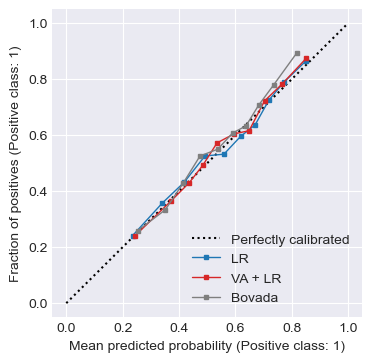
\includegraphics[width=0.9\linewidth]{figures/calib_lr_and_va.png}
\end{subfigure}%
\begin{subfigure}{.5\linewidth}
  \centering
  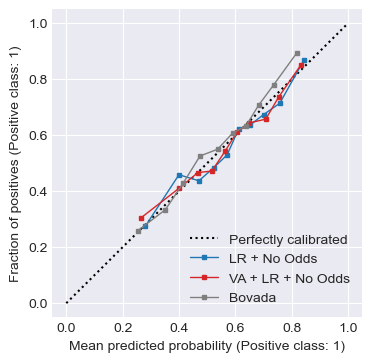
\includegraphics[width=0.9\linewidth]{figures/calib_lr_no_odds_and_va.png}
\end{subfigure}
\begin{subfigure}{.5\linewidth}
  \centering
  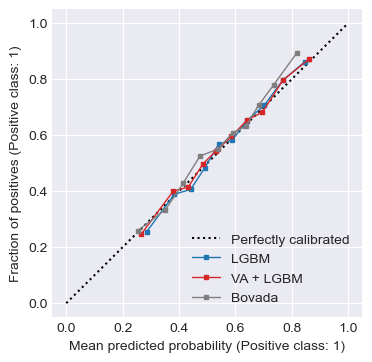
\includegraphics[width=0.9\linewidth]{figures/calib_lightgbm_and_va.png}
\end{subfigure}%
\begin{subfigure}{.5\linewidth}
  \centering
  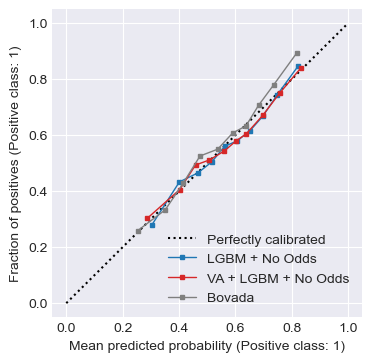
\includegraphics[width=0.9\linewidth]{figures/calib_lightgbm_no_odds_and_va.png}
\end{subfigure}
\caption{Calibration plots, comparing with and without Venn-Abers}
\end{figure}

The calibration curves indicate that all models are generally well-calibrated, closely following the ideal calibration line. While the Bovada closing odds serve as a strong baseline, some models actually align more closely with perfect calibration in higher-probability bins. Notably, removing betting odds as a feature leads to small but noticeable deviations, particularly in the mid-range probabilities (0.4 to 0.6). Venn-Abers calibration has minimal impact, suggesting that the models were already well-calibrated. Additionally, logistic regression and LightGBM exhibit similar calibration performance.


\section{Betting Results}

To analyze the betting performance of each model pipeine and strategy combination, we look at several different quantities:
\begin{enumerate}
    \item Profit, calculated as the end bankroll minus the initial bankroll.

    \item Total bets, which gives insight into how conservatively we would place bets.

    \item Yield, calculated as
    $$\frac{\text{Total returned} - \text{Total wagered}}{\text{Total wagered}} \times 100\%,$$
    which measures betting efficiency.

    \item Maximum drawdown (MDD), calculated as the worst peak-to-trough percent bankroll loss suffered during the backtest period, which reflects how risky the strategy is.

    \item Adjusted $p$-value, calculated from the Monte Carlo simulations and applying a Bonferroni correction.
\end{enumerate}
We list the full results in Table \ref{betting_results}.


\tiny
\begin{table}[!htb]
\centering
\resizebox{\linewidth}{!}{%
\begin{tabular}{llrrrrrr} 
\toprule
Model Pipeline                       & Betting Strategy                             & Fraction & Profit (\$) & Total Bets & Yield (\%) & MDD (\%) & Adj. $p$-value         \\ 
\toprule
\multirow{3}{*}{LR}                  & \multirow{3}{*}{Simultaneous Kelly}          & 0.10     & 1318.98     & 1178       & 6.40       & -22.04   & \multirow{3}{*}{0.0516}  \\
                                     &                                              & 0.15     & 2159.40     & 1196       & 5.25       & -32.02   &                          \\
                                     &                                              & 0.25     & 3763.63     & 1201       & 3.47       & -50.46   &                          \\ 
\midrule
\multirow{3}{*}{LR + No odds}        & \multirow{3}{*}{Simultaneous Kelly}          & 0.10     & -114.95     & 1810       & -0.53      & -40.19   & \multirow{3}{*}{0.9083}  \\
                                     &                                              & 0.15     & -411.12     & 1827       & -1.54      & -54.63   &                          \\
                                     &                                              & 0.25     & -868.45     & 1800       & -3.92      & -83.78   &                          \\ 
\midrule
\multirow{6}{*}{VA + LR}             & \multirow{3}{*}{Simultaneous Kelly}          & 0.10     & 430.80      & 1445       & 2.24       & -34.74   & \multirow{3}{*}{0.3528}  \\
                                     &                                              & 0.15     & 541.39      & 1469       & 1.57       & -48.37   &                          \\
                                     &                                              & 0.25     & 475.41      & 1477       & 0.63       & -72.25   &                          \\ 
\cmidrule{2-8}
                                     & \multirow{3}{*}{Distributional Robust Kelly} & 0.10     & 338.04      & 609        & 7.47       & -16.36   & \multirow{3}{*}{0.3780}  \\
                                     &                                              & 0.15     & 517.06      & 624        & 6.74       & -23.78   &                          \\
                                     &                                              & 0.25     & 875.65      & 642        & 5.48       & -37.05   &                          \\ 
\midrule
\multirow{6}{*}{VA + LR + No odds}   & \multirow{3}{*}{Simultaneous Kelly}          & 0.10     & -181.54     & 1865       & -0.78      & -45.45   & \multirow{3}{*}{1.0000}  \\
                                     &                                              & 0.15     & -479.29     & 1876       & -1.63      & -62.94   &                          \\
                                     &                                              & 0.25     & -895.77     & 1852       & -3.52      & -88.68   &                          \\ 
\cmidrule{2-8}
                                     & \multirow{3}{*}{Distributional Robust Kelly} & 0.10     & -260.40     & 1396       & -2.28      & -34.03   & \multirow{3}{*}{1.0000}  \\
                                     &                                              & 0.15     & -451.26     & 1410       & -3.13      & -51.50   &                          \\
                                     &                                              & 0.25     & -771.00     & 1410       & -5.08      & -80.58   &                          \\ 
\midrule
\multirow{3}{*}{LGBM}                & \multirow{3}{*}{Simultaneous Kelly}          & 0.10     & 192.37      & 1610       & 0.89       & -49.20   & \multirow{3}{*}{0.5999}  \\
                                     &                                              & 0.15     & 110.14      & 1626       & 0.30       & -65.76   &                          \\
                                     &                                              & 0.25     & -292.11     & 1640       & -0.44      & -86.09   &                          \\ 
\midrule
\multirow{3}{*}{LGBM + No odds}      & \multirow{3}{*}{Simultaneous Kelly}          & 0.10     & -584.14     & 1906       & -3.29      & -68.99   & \multirow{3}{*}{1.0000}  \\
                                     &                                              & 0.15     & -815.79     & 1902       & -4.20      & -84.50   &                          \\
                                     &                                              & 0.25     & -983.20     & 1782       & -7.89      & -97.84   &                          \\ 
\midrule
\multirow{6}{*}{VA + LGBM}           & \multirow{3}{*}{Simultaneous Kelly}          & 0.10     & 258.96      & 1540       & 1.21       & -46.78   & \multirow{3}{*}{0.5111}  \\
                                     &                                              & 0.15     & 216.83      & 1554       & 0.60       & -62.81   &                          \\
                                     &                                              & 0.25     & -155.18     & 1560       & -0.23      & -83.33   &                          \\ 
\cmidrule{2-8}
                                     & \multirow{3}{*}{Distributional Robust Kelly} & 0.10     & 130.44      & 881        & 1.93       & -30.01   & \multirow{3}{*}{1.0000}  \\
                                     &                                              & 0.15     & 157.37      & 898        & 1.41       & -42.07   &                          \\
                                     &                                              & 0.25     & 142.97      & 906        & 0.65       & -60.88   &                          \\ 
\midrule
\multirow{6}{*}{VA + LGBM + No odds} & \multirow{3}{*}{Simultaneous Kelly}          & 0.10     & -551.64     & 1894       & -2.86      & -72.54   & \multirow{3}{*}{1.0000}  \\
                                     &                                              & 0.15     & -796.87     & 1899       & -3.62      & -87.02   &                          \\
                                     &                                              & 0.25     & -977.22     & 1788       & -6.24      & -97.66   &                          \\ 
\cmidrule{2-8}
                                     & \multirow{3}{*}{Distributional Robust Kelly} & 0.10     & -394.33     & 1380       & -2.57      & -62.51   & \multirow{3}{*}{1.0000}  \\
                                     &                                              & 0.15     & -600.90     & 1396       & -2.71      & -78.04   &                          \\
                                     &                                              & 0.25     & -875.21     & 1406       & -2.95      & -93.14   &                          \\
\bottomrule
\end{tabular}
}
\caption{Betting metrics by model pipeline, betting strategy, and fraction}
\label{betting_results}
\end{table}
\normalsize

First and foremost, essentially all combinations of model pipeline and betting strategy failed to achieve statistical significance after a Bonferroni correction. An exception was the logistic regression pipeline combined with simultaneous Kelly, which achieved an adjusted p-value of 0.0516. While close to conventional thresholds for significance, this still borders on marginal. This lack of significance across most setups, even when performance metrics like profit and yield appear promising, underscores the conservative nature of Bonferroni correction, but also highlights the genuine difficulty in producing a consistent, long-term edge over bookmakers, especially across multiple UFC events and time periods.

\begin{figure}[!htb]
    \centering
    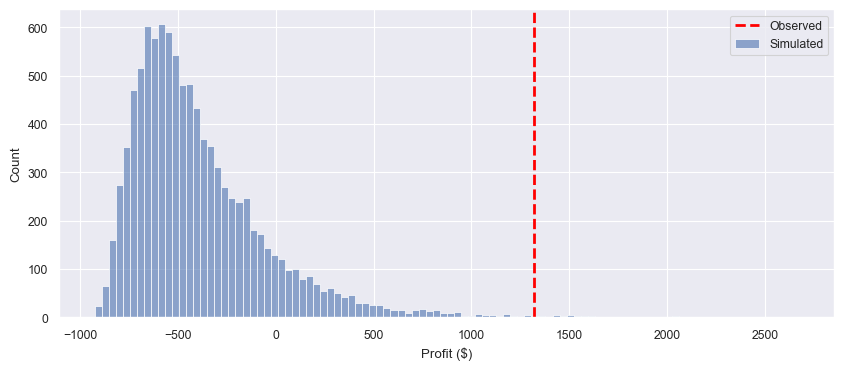
\includegraphics[width=0.8\linewidth]{figures/mc_results.png}
    \caption{Simulated profit vs. observed, LR and simultaneous Kelly $(f = 0.10)$}
\end{figure}


Next, there is a stark deterioration in betting performance when the opening odds-derived feature is omitted. Pipelines omitting this feature consistently performed worse across all model types and strategies, often posting negative profits, lower yields, and larger maximum drawdowns. For $f = 0.25$, this resulted in catastrophic losses ranging from $-77.1\%$ to $-98.3\%$ overall with respect to the initial bankroll.

\begin{figure}[!htb]
\centering
\captionsetup{justification=centering}
\begin{subfigure}{.5\linewidth}
  \centering
  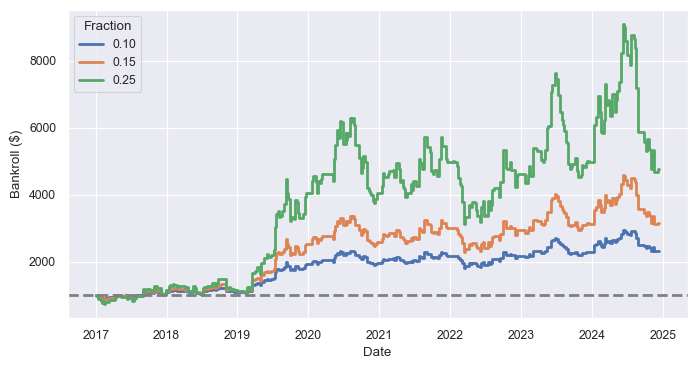
\includegraphics[width=\linewidth]{figures/bankroll_lr_simultaneous.png}
  \caption{Logistic regression}
\end{subfigure}%
\begin{subfigure}{.5\linewidth}
  \centering
  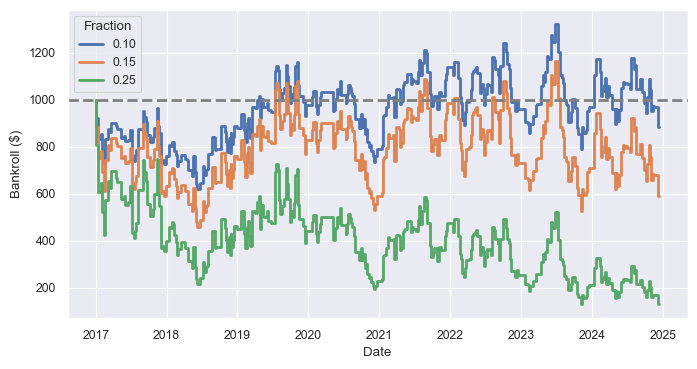
\includegraphics[width=\linewidth]{figures/bankroll_lr_no_odds_simultaneous.png}
  \caption{Logistic regression, no odds}
\end{subfigure}
\begin{subfigure}{.5\linewidth}
  \centering
  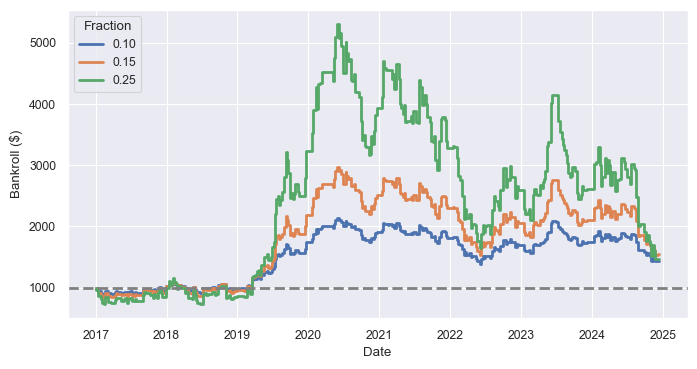
\includegraphics[width=\linewidth]{figures/bankroll_va_lr_simultaneous.png}
  \caption{Venn-Abers logistic regression}
\end{subfigure}%
\begin{subfigure}{.5\linewidth}
  \centering
  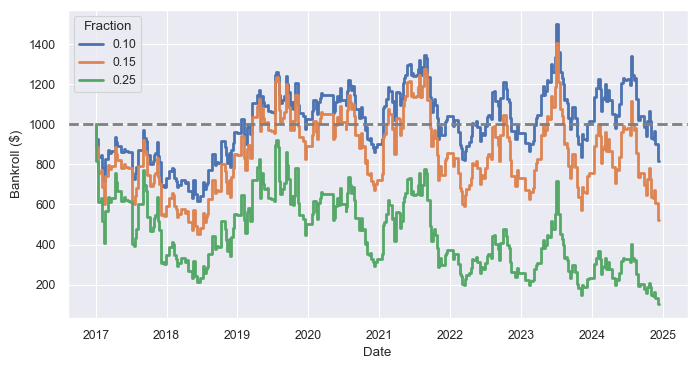
\includegraphics[width=\linewidth]{figures/bankroll_va_lr_no_odds_simultaneous.png}
  \caption{Venn-Abers logistic regression, no odds}
\end{subfigure}
\begin{subfigure}{.5\linewidth}
  \centering
  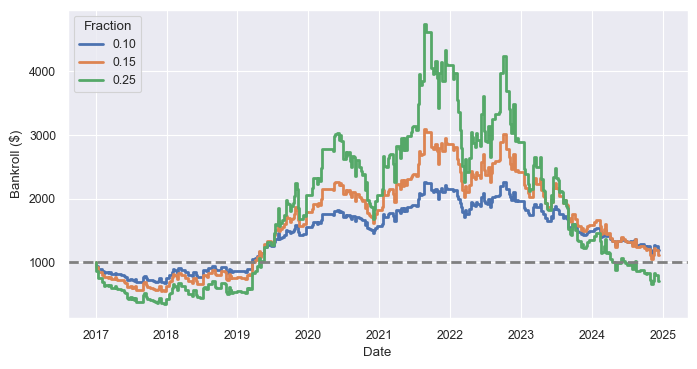
\includegraphics[width=\linewidth]{figures/bankroll_lightgbm_simultaneous.png}
  \caption{LightGBM}
\end{subfigure}%
\begin{subfigure}{.5\linewidth}
  \centering
  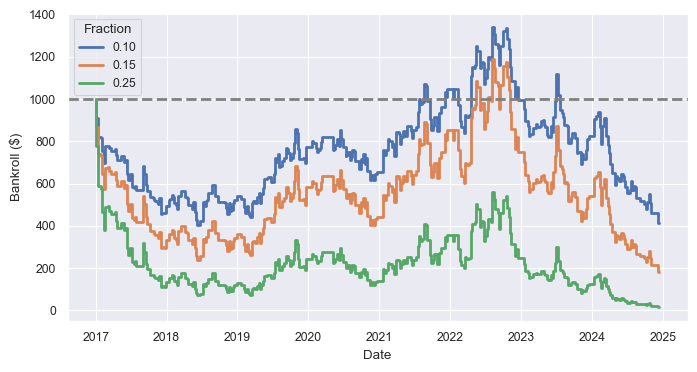
\includegraphics[width=\linewidth]{figures/bankroll_lightgbm_no_odds_simultaneous.png}
  \caption{LightGBM, no odds}
\end{subfigure}
\begin{subfigure}{.5\linewidth}
  \centering
  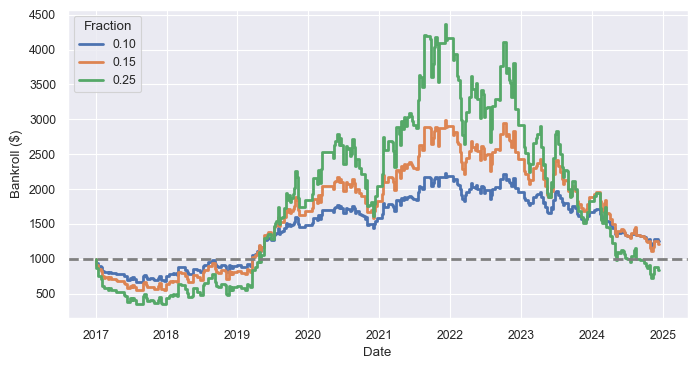
\includegraphics[width=\linewidth]{figures/bankroll_va_lightgbm_simultaneous.png}
  \caption{Venn-Abers LightGBM}
\end{subfigure}%
\begin{subfigure}{.5\linewidth}
  \centering
  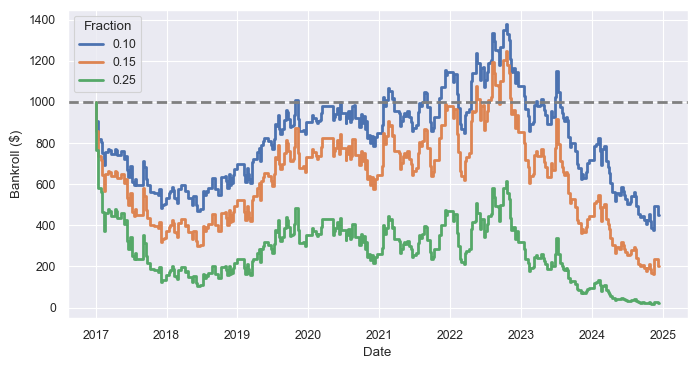
\includegraphics[width=\linewidth]{figures/bankroll_va_lightgbm_no_odds_simultaneous.png}
  \caption{Venn-Abers LightGBM, no odds}
\end{subfigure}
\caption{Bankroll over time for all simultaneous Kelly strategy combinations}
\end{figure}


Interestingly though perhaps unsurprisingly, there appears to be a meaningful relationship between out-of-sample predictive performance (log loss) and betting outcomes. Pipelines that showed lower log loss over the backtest data such as logistic regression and Venn-Abers logistic regression tended to yield better betting performance than those with higher log loss, such as LightGBM-based pipelines and those omitting the opening odds-derived feature. This reinforces the link between well-calibrated probabilistic predictions and successful wagering strategies in that accurate win probabilities are a prerequisite for exploiting mispriced lines when using value betting-based strategies.

The influence of fractional Kelly sizing is also notable. Lower Kelly fractions (e.g., 0.10) typically led to better yields and reduced maximum drawdowns, albeit at the cost of reduced absolute profit. This aligns with established theoretical expectations and reflects a more risk-conscious approach that trades off some upside for greater stability and efficiency.

Finally, pipelines utilizing Venn-Abers calibration in combination with distributional robust Kelly produced far fewer bets, indicating a more conservative betting posture. While this frequently improved yield and limited drawdowns, it also constrained profit potential due to smaller action volume. Nevertheless, the benefit of DRK in taming variance and providing tighter probabilistic guarantees is evident in its risk-adjusted performance. That said, pipelines based on LightGBM models were uniformly worse than those built on logistic regression, demonstrating not only poorer test log loss but also inferior betting performance metrics, which could be due to LightGBM’s overfitting, instability in smaller datasets, or simply from not tuning hyperparameters carefully enough.


\begin{figure}[!htb]
\centering
\captionsetup{justification=centering}
\begin{subfigure}{.5\linewidth}
  \centering
  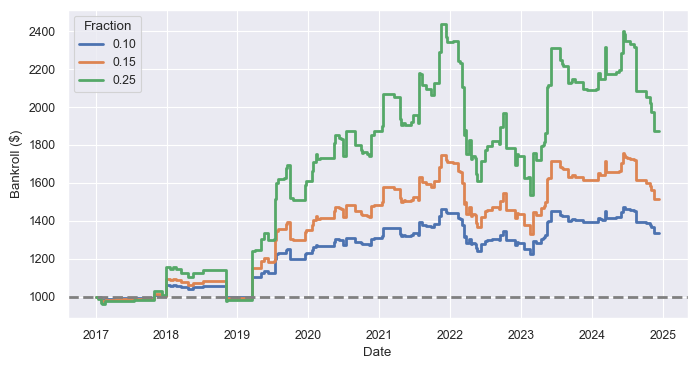
\includegraphics[width=\linewidth]{figures/bankroll_va_lr_distributional_robust.png}
  \caption{Venn-Abers logistic regression}
\end{subfigure}%
\begin{subfigure}{.5\linewidth}
  \centering
  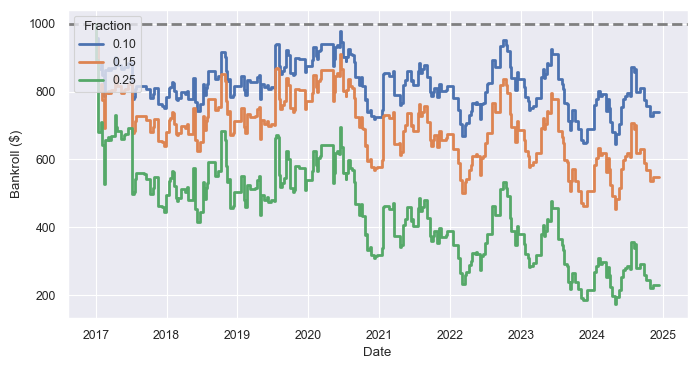
\includegraphics[width=\linewidth]{figures/bankroll_va_lr_no_odds_distributional_robust.png}
  \caption{Venn-Abers logistic regression, no odds}
\end{subfigure}
\begin{subfigure}{.5\linewidth}
  \centering
  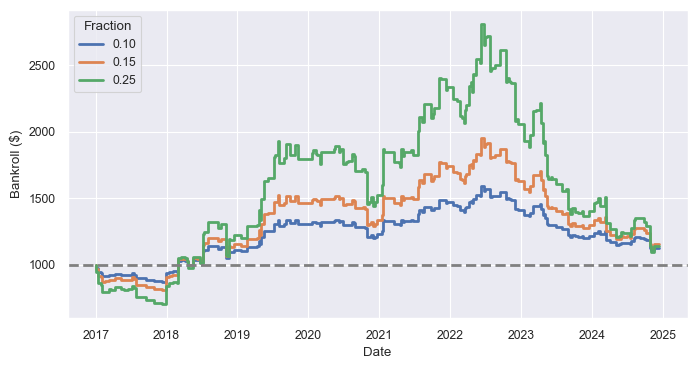
\includegraphics[width=\linewidth]{figures/bankroll_va_lightgbm_distributional_robust.png}
  \caption{Venn-Abers LightGBM}
\end{subfigure}%
\begin{subfigure}{.5\linewidth}
  \centering
  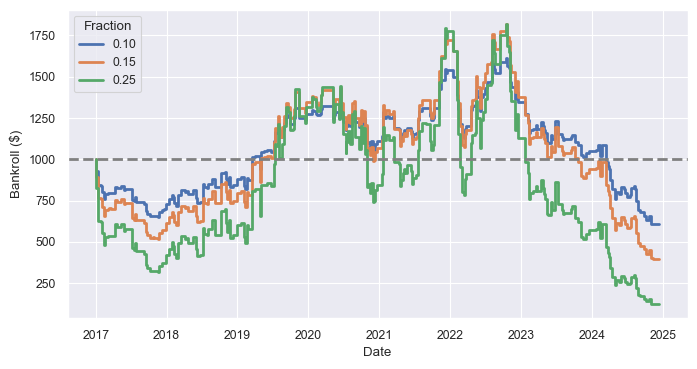
\includegraphics[width=\linewidth]{figures/bankroll_va_lightgbm_no_odds_distributional_robust.png}
  \caption{Venn-Abers LightGBM, no odds}
\end{subfigure}
\caption{Bankroll over time for all distributional robust Kelly strategy combinations}
\end{figure}



\section{Case Study: LR and Simultaneous Kelly}

While the logistic regression and simultaneous Kelly combination clearly delivered the strongest performance, both in terms of quality of probability estimates and long-term profitability, a healthy skeptic should question whether this edge is truly robust. For instance, one may point out how most of the profits come from major bankroll growth during 2019 and 2020, followed by a prolonged period of stagnant growth and volatility. To build confidence in our findings and better understand where our approach succeeds or fails, we turn to a deeper case study of this specific configuration.

We begin by examining which features were most influential in the model pipeline, based on how frequently they were selected during feature selection and the average absolute weight assigned to each over the backtest period. Then, we analyze where our model’s edge breaks down by identifying subsets of fights where performance with respect to log loss and Brier score was consistently poor compared to the bookmakers. Finally, guided by these insights, we re-run our backtest with these fight types omitted to evaluate whether profitability persists or even improves within this more selective market.


\subsection{Feature Importances}

Unlike tree-based models, where feature importance is inherently more interpretable, the notion of "importance" in linear models such as logistic regression is less well-defined. Permutation importance is a model-agnostic option, but in turn is costly to compute and tedious to implement such that it respects our retuning and refitting procedure during backtesting. As a result, to explore which features were most relevant to our model pipeline, we adopt a practical, frequency- and magnitude-based approach.

Specifically, we evaluate feature relevance by tracking two metrics across the backtest period: (1) how often each feature was selected during the feature selection process, and (2) the average absolute value of its logistic regression coefficient. To compute these, we re-simulate our backtest procedure, refitting the model after each event using hyperparameters determined on data available up to the most recent full year. For each refit, we increment a count for any feature that passes the variance threshold and top-k selection based on mutual information. We also extract the absolute value of that feature’s coefficient from the fitted logistic regression model. If a feature was not selected during a given refit, it is assigned a coefficient of zero. Finally, we average these absolute coefficient values across all refits to arrive at a summary measure.

\begin{figure}[!htb]
\centering
\captionsetup{justification=centering}
\begin{subfigure}{\linewidth}
  \centering
  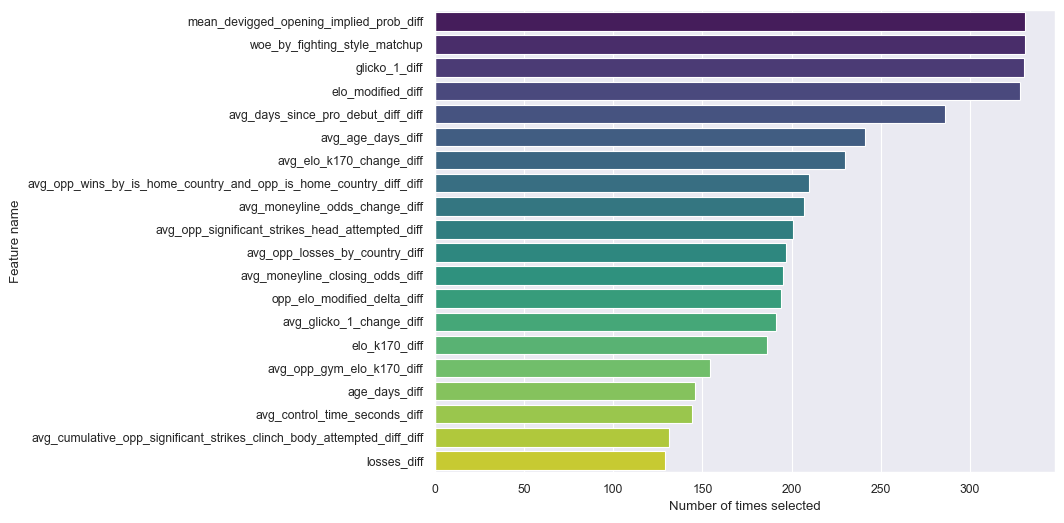
\includegraphics[width=\linewidth]{figures/lr_feature_selection_freq.png}
\end{subfigure}\\
\begin{subfigure}{\linewidth}
  \centering
  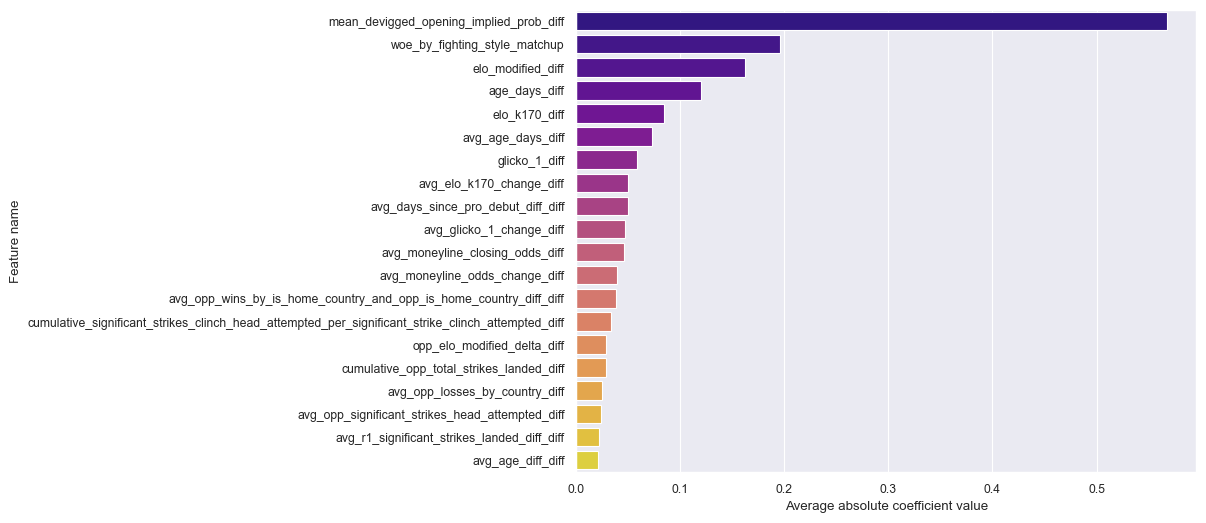
\includegraphics[width=\linewidth]{figures/lr_feature_avg_abs_coef.png}
\end{subfigure}
\caption{Top 20 features by frequency of selection and average absolute coefficient value}
\label{feature_importances}
\end{figure}

The plots in Figure \ref{feature_importances} show the top 20 features ranked by each criterion. There is a substantial amount of overlap between the two rankings, indicating that many features are both frequently selected and consistently influential. Notably, the opening odds-derived feature stands out with the highest average absolute coefficient value. This aligns with expectations, as odds represent a distilled, crowd-sourced probability estimate. However, it is crucial to note that the model is not overly reliant on this single feature with many other features also play meaningful albeit smaller roles based on the average absolute coefficient values without being overshadowed. Importantly, they span multiple data sources; this diversity of signals underscores the strength of our entire approach: the model leverages complementary information from a wide array of inputs in a way that would not have been possible without considering data sources other than UFC Stats, leading to more nuanced predictions than any single feature could provide on its own. To make this more clear, we take the union of the two sets of 20 features and list all sources from which they were created in Table \ref{feature_sources}. Given that 8 out of the 10 sources are represented in only these 24 features, it should be clear there is a substantial value-add from considering nontraditional data.

\tiny 
\begin{table}[!htb]
\centering
\resizebox{\linewidth}{!}{%
\begin{tabular}{rl} 
\toprule
Feature Name                                                                                                 & Data Sources                                                     \\ 
\toprule
age\_days\_diff                                                                                              & ESPN, FightOdds.io, MMA Decisions, Sherdog, Tapology, UFC Stats  \\
avg\_age\_days\_diff                                                                                         & ESPN, FightOdds.io, MMA Decisions, Sherdog, Tapology, UFC Stats  \\
avg\_age\_diff\_diff                                                                                         & ESPN, FightOdds.io, MMA Decisions, Sherdog, Tapology, UFC Stats  \\
avg\_control\_time\_seconds\_diff                                                                            & UFC Stats                                                        \\
avg\_cumulative\_opp\_significant\_strikes\_clinch\_body\_attempted\_diff\_diff                              & ESPN                                                             \\
avg\_days\_since\_pro\_debut\_diff\_diff                                                                     & Fight Matrix                                                     \\
avg\_elo\_k170\_change\_diff                                                                                 & Fight Matrix                                                     \\
avg\_glicko\_1\_change\_diff                                                                                 & Fight Matrix                                                     \\
avg\_moneyline\_closing\_odds\_diff                                                                          & Best Fight Odds, FightOdds.io, Tapology                          \\
avg\_moneyline\_odds\_change\_diff                                                                           & Best Fight Odds, FightOdds.io, Tapology                          \\
avg\_opp\_gym\_elo\_k170\_diff                                                                               & Fight Matrix, Tapology                                           \\
avg\_opp\_losses\_by\_country\_diff                                                                          & Sherdog                                                          \\
avg\_opp\_significant\_strikes\_head\_attempted\_diff                                                        & UFC Stats                                                        \\
avg\_opp\_wins\_by\_is\_home\_country\_and\_opp\_is\_home\_country\_diff\_diff                               & Sherdog                                                          \\
avg\_r1\_significant\_strikes\_landed\_diff\_diff                                                            & UFC Stats                                                        \\
cumulative\_opp\_total\_strikes\_landed\_diff                                                                & UFC Stats                                                        \\
cumulative\_significant\_strikes\_clinch\_head\_attempted\_per\_significant\_strike\_clinch\_attempted\_diff & ESPN                                                             \\
elo\_k170\_diff                                                                                              & Fight Matrix                                                     \\
elo\_modified\_diff                                                                                          & Fight Matrix                                                     \\
glicko\_1\_diff                                                                                              & Fight Matrix                                                     \\
losses\_diff                                                                                                 & Fight Matrix, Sherdog                                            \\
mean\_devigged\_opening\_implied\_prob\_diff                                                                 & Best Fight Odds, FightOdds.io                                    \\
opp\_elo\_modified\_delta\_diff                                                                              & Fight Matrix                                                     \\
woe\_by\_fighting\_style\_matchup                                                                            & FightOdds.io                                                     \\
\bottomrule
\end{tabular}
}
\caption{Feature names and corresponding data sources}
\label{feature_sources}
\end{table}
\normalsize


\subsection{Edge Analysis}

We established in the betting results section that there is a clear relationship between a model's log loss (and Brier score) and profitability, and so we can use this as a proxy for understanding where the logistic regression and simultaneous Kelly combination is making losing bets on average for certain fight categories.

Table \ref{case_study_by_year} presents a year-by-year comparison of log loss and Brier scores between our model and Bovada's implied probabilities. Notably, our model outperforms Bovada in 2019 and 2020, as evidenced by lower values in both metrics. The noticeable spike in Bovada’s log loss and Brier score in 2019 may reflect a structural change in the UFC betting landscape---perhaps a regime shift or an influx of less predictable fight dynamics that the bookmakers struggled to adapt to. This trend appears to carry into 2020 and 2021, though it is likely confounded by the COVID-19 pandemic, which caused widespread event disruptions and unusual conditions (e.g., fights without live audiences). From 2022 onward, however, Bovada’s closing odds improve steadily, and our model no longer consistently outperforms the market. This tightening of the sportsbook’s predictions may explain the stagnation observed in our backtest bankroll during the same period, pointing to potential edge decay.
 

\begin{table}[!htb]
\centering
\begin{tabular}{@{}cccrcccr@{}}
\toprule
\multirow{2}{*}{Year} & \multicolumn{3}{c}{Log Loss}                                                               & \multirow{2}{*}{}    & \multicolumn{3}{c}{Brier Score}                    \\ \cmidrule(lr){2-4} \cmidrule(l){6-8} 
                      & Model                        & Bovada                       & \multicolumn{1}{c}{$\Delta$} &                      & Model    & Bovada   & \multicolumn{1}{c}{$\Delta$} \\ \midrule
2017                  & 0.614738                     & 0.609460                     & 0.005277                     &                      & 0.212572 & 0.210317 & 0.002256                     \\
2018                  & \multicolumn{1}{l}{0.597811} & \multicolumn{1}{l}{0.597080} & 0.000731                     & \multicolumn{1}{l}{} & 0.206408 & 0.205833 & 0.000575                     \\
2019                  & 0.624346                     & 0.636898                     & -0.012552                    &                      & 0.217742 & 0.223757 & -0.006016                    \\
2020                  & 0.611094                     & 0.617461                     & -0.006367                    &                      & 0.211575 & 0.214045 & -0.002470                    \\
2021                  & 0.622634                     & 0.621523                     & 0.001110                     &                      & 0.217409 & 0.216309 & 0.001100                     \\
2022                  & 0.599701                     & 0.597913                     & 0.001788                     &                      & 0.207473 & 0.205662 & 0.001811                     \\
2023                  & 0.608926                     & 0.602462                     & 0.006465                     &                      & 0.210956 & 0.207674 & 0.003282                     \\
2024                  & 0.586208                     & 0.583386                     & 0.002822                     &                      & 0.199778 & 0.198925 & 0.000853                     \\ \bottomrule
\end{tabular}
\caption{Model pipeline and sportsbook log loss and Brier score by year}
\label{case_study_by_year}
\end{table}

While there are likely much more complex dynamics at play, we hypothesize the structural change in 2019 may be in part due to the following related reasons:
\begin{enumerate}
    \item An increase in the number of non-pay-per-view events, which tend to host matchups of inferior quality between lower profile fighters.

    \item An increase in the number of bouts in women's divisions. Women fight very differently from men.

    \item An increase in the number of debuting fighters. Recall that comparative features are automatically set to a value of zero when there is missing data.
\end{enumerate}
Plotting the number of bouts per year segmented by the above facets seems to provide some evidence that supports this hypothesis.

\begin{figure}[!htb]
\centering
\captionsetup{justification=centering}
\begin{subfigure}{0.42\linewidth}
  \centering
  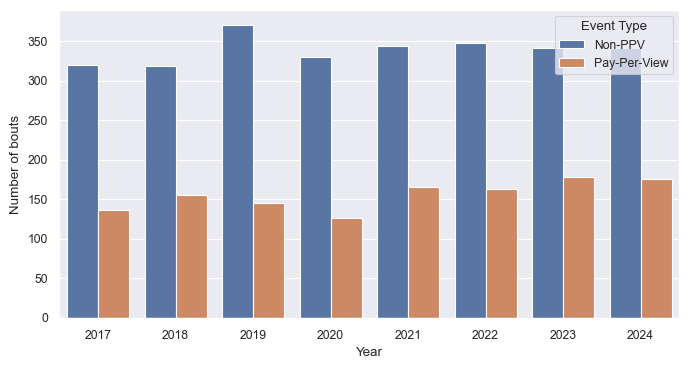
\includegraphics[width=\linewidth]{figures/event_type_by_year.png}
\end{subfigure}
\begin{subfigure}{0.42\linewidth}
  \centering
  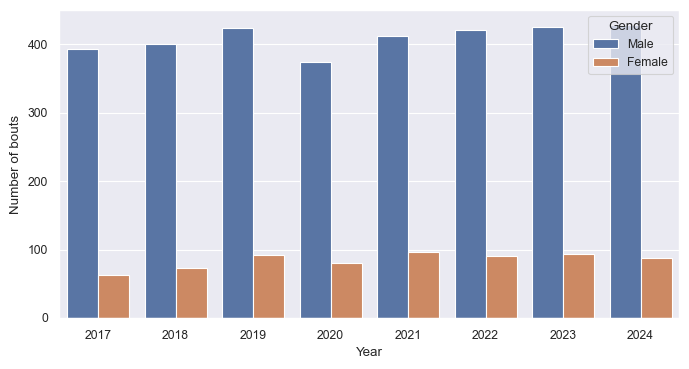
\includegraphics[width=\linewidth]{figures/gender_by_year.png}
\end{subfigure}\\
\begin{subfigure}{0.42\linewidth}
  \centering
  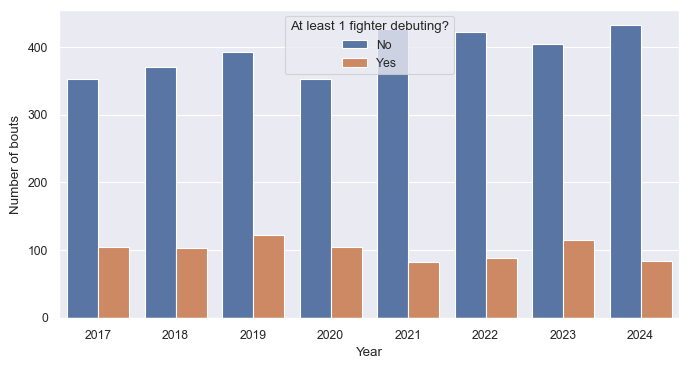
\includegraphics[width=\linewidth]{figures/debuts_by_year.png}
\end{subfigure}
\caption{Number of bouts per year by event type, gender, and debuts}
\end{figure}

We can see a noticeable increase in fights belonging to non-PPV events in the top left subfigure, with smaller increases in fights in women's divisions and those involving at least one debuting fighter. To further investigate this, we repeat the comparison of log loss and Brier scores between our logistic regression model and the sportsbook for event type. As postulated, while our model outperforms the betting market for fights on pay-per-view events, we trail slightly behind for non-PPV events like Fight Nights.


\begin{table}[!htb]
\centering
\begin{tabular}{@{}cccrcccr@{}}
\toprule
\multirow{2}{*}{Event Type} & \multicolumn{3}{c}{Log Loss}                       & \multirow{2}{*}{} & \multicolumn{3}{c}{Brier Score}                    \\ \cmidrule(lr){2-4} \cmidrule(l){6-8} 
                        & Model    & Bovada   & \multicolumn{1}{c}{$\Delta$} &                   & Model    & Bovada   & \multicolumn{1}{c}{$\Delta$} \\ \midrule
Pay-Per-View            & 0.593012 & 0.596247 & -0.003235                    &                   & 0.203459 & 0.204517 & -0.001057                    \\
Non-PPV             & 0.614957 & 0.613594 & 0.001363                     &                   & 0.213644 & 0.212900 & 0.000744                     \\ \bottomrule
\end{tabular}
\caption{Model pipeline and sportsbook log loss and Brier score by event type}
\end{table}


Similarly, we see that our model performs extremely poorly on women's fights, highlighting a massive weakness in using a single universal model for all fights. This raises an interesting question as to whether or not building and maintaining separate men's and women's models could help improve overall performance at the expense of less training data for each, especially for the women's only model.


\begin{table}[!htb]
\centering
\begin{tabular}{@{}cccrcccr@{}}
\toprule
\multirow{2}{*}{Gender} & \multicolumn{3}{c}{Log Loss}                       & \multirow{2}{*}{} & \multicolumn{3}{c}{Brier Score}                    \\ \cmidrule(lr){2-4} \cmidrule(l){6-8} 
                        & Model    & Bovada   & \multicolumn{1}{c}{$\Delta$} &                   & Model    & Bovada   & \multicolumn{1}{c}{$\Delta$} \\ \midrule
Male                    & 0.603392 & 0.606017 & -0.002625                    &                   & 0.208329 & 0.209354 & -0.001025                    \\
Female                  & 0.630458 & 0.618340 & 0.012118                     &                   & 0.220585 & 0.214636 & 0.005949                     \\ \bottomrule
\end{tabular}
\caption{Model pipeline and sportsbook log loss and Brier score by gender of both fighters}
\end{table}

We can expand on the above analysis and continue to segment by weight class, which reveals that even within men's and women's fights, our model's advantage and disadvantage respectively are not universal across weight classes. In particular, for men's weight classes our model falls slightly behind Bovada for Middleweight and Heavyweight fights, but struggles substantially with Flyweight fights. It is unclear why there is such a large discrepancy for this weight class; it may be that Flyweights fight much differently in that they tend to have much higher pace and output. Similarly, most of the struggles with women's fights comes from those in the Women's Bantamweight division. On the other hand, our model slightly outperforms the sportsbook for Women's Featherweight bouts. However, this is likely an artifact of sample size; the division has essentially been nonexistent and completely inactive in recent years.


\begin{table}[!htb]
\footnotesize
\centering
\begin{tabular}{@{}cccrlccr@{}}
\toprule
\multirow{2}{*}{Weight Class}  & \multicolumn{3}{c}{Log Loss}                       & \multicolumn{1}{c}{\multirow{2}{*}{}} & \multicolumn{3}{c}{Brier Score}                    \\ \cmidrule(lr){2-4} \cmidrule(l){6-8} 
                               & Model    & Bovada   & \multicolumn{1}{c}{$\Delta$} & \multicolumn{1}{c}{}                  & Model    & Bovada   & \multicolumn{1}{c}{$\Delta$} \\ \midrule
Flyweight (125 lb)             & 0.616030 & 0.599282 & 0.016748                     & \multicolumn{1}{c}{}                  & 0.213518 & 0.206364 & 0.007154                     \\
Bantamweight (135 lb)          & 0.565713 & 0.574666 & -0.008953                    &                                       & 0.191710 & 0.194942 & -0.003233                    \\
Featherweight (145 lb)         & 0.630611 & 0.632581 & -0.001970                    &                                       & 0.222071 & 0.222485 & -0.000414                    \\
Lightweight (155 lb)           & 0.594020 & 0.601535 & -0.007516                    &                                       & 0.202938 & 0.206925 & -0.003987                    \\
Welterweight (170 lb)          & 0.594951 & 0.609887 & -0.014936                    &                                       & 0.204211 & 0.211111 & -0.006900                    \\
Middleweight (185 lb)          & 0.606203 & 0.599149 & 0.007054                     &                                       & 0.209518 & 0.205799 & 0.003720                     \\
Light Heavyweight (205 lb)     & 0.643278 & 0.637065 & 0.006213                     &                                       & 0.226161 & 0.223313 & 0.002848                     \\
Heavyweight (265 lb)           & 0.601697 & 0.602283 & -0.000585                    &                                       & 0.208332 & 0.207261 & 0.001071                     \\
Women's Strawweight (115 lb)   & 0.631688 & 0.614281 & 0.017407                     &                                       & 0.221299 & 0.212762 & 0.008537                     \\
Women's Flyweight (125 lb)     & 0.639230 & 0.638435 & 0.000794                     &                                       & 0.224458 & 0.223610 & 0.000848                     \\
Women's Bantamweight (135 lb)  & 0.637887 & 0.614512 & 0.023376                     &                                       & 0.223465 & 0.212768 & 0.010697                     \\
Women's Featherweight (145 lb) & 0.490214 & 0.493945 & -0.003731                    &                                       & 0.161755 & 0.160670 & 0.001085                     \\
Catch Weight (Variable)        & 0.579667 & 0.581412 & -0.001745                    & \multicolumn{1}{c}{}                  & 0.194415 & 0.200654 & -0.006239                    \\ \bottomrule
\end{tabular}
\caption{Model pipeline and sportsbook log loss and Brier score by weight class}
\end{table}
\normalsize

Lastly, as expected our model struggles significantly for fights where at least one fighter is making their UFC debut. As mentioned earlier, this is likely due to many fighter-level striking and grappling features based on data from UFC Stats and ESPN not being defined until after a fighter has fought at least once within the promotion, causing the final difference feature to be set to zero. One potential method at mitigating this at least for cases where exactly one fighter is debuting is to effectively smooth the fighter-level features using a Bayesian approach and choosing a prior based on empirical Bayes. This could be implemented at the weight class level for each feature such that the global mean for a particular weight class based on other fighters in that same group is initially heavily weighed. Another approach could be to acquire striking and grappling data from other promotions, although this would require some combination of additional tedious scraping and paying for proprietary datasets. However, this would probably lead to more issues due to gaps in the data and a continuously growing number of data source dependencies.


\begin{table}[!htb]
\centering
\begin{tabular}{@{}cccrcccr@{}}
\toprule
\multirow{2}{*}{UFC Experience} & \multicolumn{3}{c}{Log Loss}                       & \multirow{2}{*}{}    & \multicolumn{3}{c}{Brier Score}                    \\ \cmidrule(lr){2-4} \cmidrule(l){6-8} 
                                & Model    & Bovada   & \multicolumn{1}{c}{$\Delta$} &                      & Model    & Bovada   & \multicolumn{1}{c}{$\Delta$} \\ \midrule
Both debuting                   & 0.607946 & 0.579237 & 0.028709                     &                      & 0.210271 & 0.196018 & 0.014253                     \\
One fighter debuting            & 0.573801 & 0.560372 & 0.013429                    & \multicolumn{1}{l}{} & 0.195112 & 0.189045 & 0.006067                     \\
Both at least 1 fight           & 0.615511 & 0.619609 & -0.004098                    & \multicolumn{1}{l}{} & 0.213782 & 0.215412 & -0.001630                    \\
Both at least 3 fights          & 0.614461 & 0.617389 & -0.002927                    & \multicolumn{1}{l}{} & 0.213161 & 0.214277 & -0.001116                    \\
Both at least 5 fights          & 0.613856 & 0.617412 & -0.003556                    &                      & 0.212762 & 0.214238 & -0.001476                   \\ \bottomrule
\end{tabular}
\caption{Model pipeline and sportsbook log loss and Brier score by experience in the UFC}
\end{table}


\subsection{Fight Subset Analysis}

As a final experiment, based on our edge analysis we rerun the entire backtesting procedure for logistic regression and simultaneous Kelly with fights in women's divisions and those that involve at least one fighter making their UFC debut removed from all training and testing data. The motivation behind this is to investigate whether or not focusing on fights that our original model performed better for and specifically optimizing further for those fights improves our edge. For convenience, we did not redefine any of the features that were not specific to a particular fighter (i.e., event-level and bout-level features) such that they were created from this new restricted subset. In other words, some of our features still use information from women's and debut fights in their construction and were not changed.

With this filtering, there were 2622 bouts in the backtest period as opposed to 3960. Initially, this significant reduction in test data raised concerns about not having a sufficient number of bets placed, since only around 30\% of bouts were considered betting opportunities by this model and strategy combination in the original series of experiments. However, this did not end up being an issue as we will discuss later. We will again cover model results first followed by betting results and recreate the previous tables and figures.

\begin{table}[!htb]
\centering
\begin{tabular}{@{}lcc@{}}
\toprule
                    & Log Loss & Brier Score \\ \midrule
Logistic Regression & 0.611250 & 0.211724    \\
Bovada Sportsbook   & 0.616538 & 0.214093    \\ \bottomrule
\end{tabular}
\caption{Model metrics over backtest period for fight subset, compared with closing odds}
\end{table}

\begin{figure}[!htb]
    \centering
    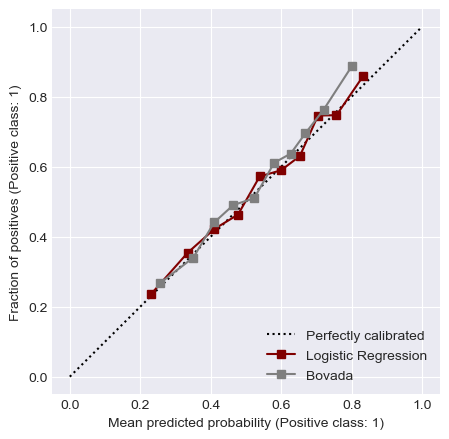
\includegraphics[width=0.45\linewidth]{figures/calib_case_study.png}   
    \caption{Calibration plot for fight subset}
\end{figure}

After restricting the dataset to exclude women's fights and fighter debuts, we observe a more pronounced performance advantage for our logistic regression model over the Bovada sportsbook than in the full dataset. This suggests that women's fights indeed are governed by fundamentally different dynamics than men's fights and attempting to model both with the same set of signals is challenging without harming overall model performance. Moreover, focusing on bouts with more ``established" fighters allows our model to more effectively utilize the predictive signals from striking and grappling statistics since they are more likely to be nonzero. The corresponding calibration plot reinforces the reliability of our model’s probability estimates. The logistic regression curve closely tracks the diagonal across most of the probability range, indicating that the model is reasonably well-calibrated out of the box. The Bovada implied probabilities are also well-calibrated, and it is not immediately clear which of the two is better calibrated based on this visual comparison alone. Both curves show some minor deviations in the tails, but largely fall within acceptable bounds.

\begin{table}[!htb]
\centering
\begin{tabular}{cccrlccr} 
\toprule
\multirow{2}{*}{Year} & \multicolumn{3}{c}{Log Loss}                       &  & \multicolumn{3}{c}{Brier Score}                     \\ 
\cmidrule[\heavyrulewidth]{2-4}\cmidrule[\heavyrulewidth]{6-8}
                      & Model    & Bovada   & \multicolumn{1}{c}{$\Delta$} &  & Model    & Bovada   & \multicolumn{1}{c}{$\Delta$}  \\ 
\toprule
2017                  & 0.624103 & 0.621143 & 0.002960                     &  & 0.216520 & 0.215718 & 0.000803                      \\
2018                  & 0.626382 & 0.611979 & 0.014404                     &  & 0.219256 & 0.212561 & 0.006695                      \\
2019                  & 0.623939 & 0.642335 & -0.018396                    &  & 0.217112 & 0.226449 & -0.009337                     \\
2020                  & 0.639725 & 0.631033 & 0.008693                     &  & 0.223882 & 0.220448 & 0.003434                      \\
2021                  & 0.623313 & 0.640873 & -0.017559                    &  & 0.217423 & 0.224868 & -0.007446                     \\
2022                  & 0.577213 & 0.593502 & -0.016290                    &  & 0.196915 & 0.203635 & -0.006720                     \\
2023                  & 0.601616 & 0.613623 & -0.012007                    &  & 0.207767 & 0.212346 & -0.004578                     \\
2024                  & 0.583331 & 0.583660 & -0.000329                    &  & 0.199085 & 0.199324 & -0.000238                     \\
\bottomrule
\end{tabular}
\caption{Model and sportsbook log loss and Brier score by year, fight subset}
\end{table}

\begin{table}[!htb]
\centering
\begin{tabular}{@{}cccrcccr@{}}
\toprule
\multirow{2}{*}{Event Type} & \multicolumn{3}{c}{Log Loss}                       & \multirow{2}{*}{} & \multicolumn{3}{c}{Brier Score}                    \\ \cmidrule(lr){2-4} \cmidrule(l){6-8} 
                        & Model    & Bovada   & \multicolumn{1}{c}{$\Delta$} &                   & Model    & Bovada   & \multicolumn{1}{c}{$\Delta$} \\ \midrule
Pay-Per-View            & 0.589874 & 0.597564 & -0.007690                    &                   & 0.201896 & 0.205361 & -0.003465                    \\
Non-PPV             & 0.621889 & 0.625981 & -0.004092                     &                   & 0.216614 & 0.218438 & -0.001824                     \\ \bottomrule
\end{tabular}
\caption{Model and sportsbook log loss and Brier score by event type, fight subset}
\end{table}

Next, we break down the log loss and Brier score comparisons again by year, event type, and weight class. We see that our model outperforms the sportsbook almost uniformly across all segmentations. Most notably, we see that this advantage persists across the last four years despite Bovada becoming sharper over time, though this edge does seem to be diminishing recently. Also, we no longer appear to fall short in non-PPV events.


\begin{table}[!htb]
\footnotesize
\centering
\begin{tabular}{@{}cccrlccr@{}}
\toprule
\multirow{2}{*}{Weight Class}  & \multicolumn{3}{c}{Log Loss}                       & \multicolumn{1}{c}{\multirow{2}{*}{}} & \multicolumn{3}{c}{Brier Score}                    \\ \cmidrule(lr){2-4} \cmidrule(l){6-8} 
                               & Model    & Bovada   & \multicolumn{1}{c}{$\Delta$} & \multicolumn{1}{c}{}                  & Model    & Bovada   & \multicolumn{1}{c}{$\Delta$} \\ \midrule
Flyweight (125 lb)             & 0.635920 & 0.618714 & 0.017206                     & \multicolumn{1}{c}{}                  & 0.222396 & 0.215153 & 0.007243                     \\
Bantamweight (135 lb)          & 0.577206 & 0.587790 & -0.010584                    &                                       & 0.196768 & 0.200515 & -0.003747                    \\
Featherweight (145 lb)         & 0.648402 & 0.655726 & -0.007324                    &                                       & 0.228579 & 0.232927 & -0.004347                    \\
Lightweight (155 lb)           & 0.593303 & 0.599683 & -0.006379                    &                                       & 0.203717 & 0.206239 & -0.002522                    \\
Welterweight (170 lb)          & 0.597877 & 0.613008 & -0.015131                    &                                       & 0.205375 & 0.212727 & -0.007351                    \\
Middleweight (185 lb)          & 0.608316 & 0.614690 & -0.006374                     &                                       & 0.209734 & 0.212484 & -0.002750                     \\
Light Heavyweight (205 lb)     & 0.654473 & 0.641892 & 0.012581                     &                                       & 0.230995 & 0.225621 & 0.005374                     \\
Heavyweight (265 lb)           & 0.602975 & 0.610443 & -0.007468                    &                                       & 0.209007 & 0.211141 & -0.002134                     \\
Catch Weight (Variable)        & 0.608679 & 0.613781 & -0.005103                    & \multicolumn{1}{c}{}                  & 0.212001 & 0.215196 & -0.003195                    \\ \bottomrule
\end{tabular}
\caption{Model and sportsbook log loss and Brier score by weight class, fight subset}
\end{table}
\normalsize

We repeat the process of quantifying feature relevance and obtain similar results as before. However, it does appear that this iteration of the model weighs the opening odds-derived feature less and values the difference between the fighters' ages significantly more. We also see features derived from fighters' past proposition betting odds and other exotic markets show up for the first time within both top 20 feature sets.

\begin{figure}[!htb]
\centering
\captionsetup{justification=centering}
\begin{subfigure}{0.8\linewidth}
  \centering
  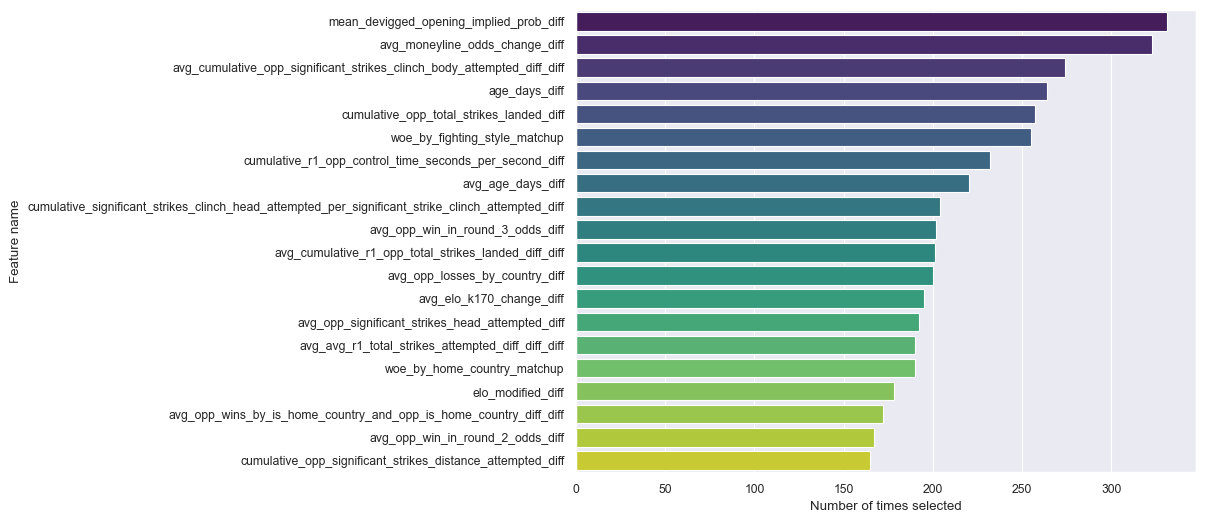
\includegraphics[width=\linewidth]{figures/lr_case_study_feature_selection_freq.png}
\end{subfigure}\\
\begin{subfigure}{0.8\linewidth}
  \centering
  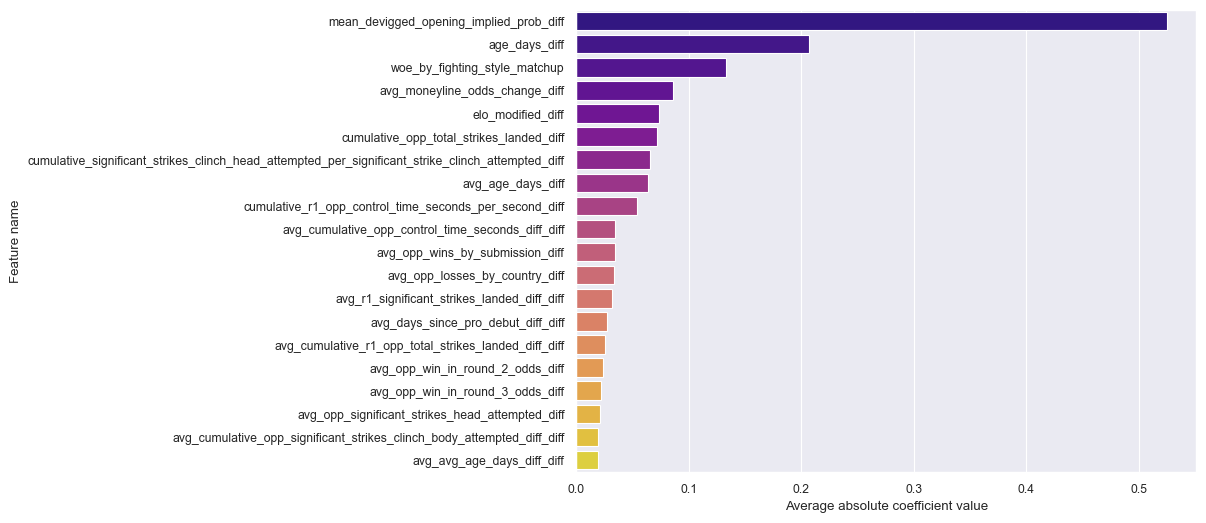
\includegraphics[width=\linewidth]{figures/lr_case_study_feature_avg_abs_coef.png}
\end{subfigure}
\caption{Top 20 features by each criteria, fight subset}
\end{figure}

Accompanying the improvements in model performance, we also observe a substantial improvement in practically every relevant betting metric. for a 10\% Kelly fraction, profit rose to \$4758.95 compared to the earlier runs, and even more dramatically at 25\% Kelly with \$43830.51 in profit. This suggests that the model’s edge is more exploitable in this more stable subset of fights. Yield remains strong across all fractions, peaking at nearly 16\% for the most conservative strategy (0.10 fraction), and a relatively modest maximum drawdown of -20.56\%, pointing to a favorable risk-reward tradeoff. Furthermore, Monte Carlo simulations reveal that the observed profit lies far in the right tail of the simulated null distribution, making it highly unlikely the result is due to chance even with any sort of reasonable correction for multiple testing.

\begin{table}[!htb]
\centering
\begin{tabular}{rrrrrr} 
\toprule
Fraction & Profit (\$) & Total Bets & Yield (\%) & MDD (\%) & Raw $p$-value            \\ 
\toprule
0.10     & 4758.95     & 964        & 15.99      & -20.56   & \multirow{3}{*}{0.0001}  \\
0.15     & 11306.91    & 974        & 14.21      & -29.42   &                          \\
0.25     & 43830.51    & 976        & 11.07      & -46.47   &                          \\
\bottomrule
\end{tabular}
\caption{Betting metrics by fraction, fight subset}
\end{table}

\begin{figure}[!htb]
\centering
\captionsetup{justification=centering}
\begin{subfigure}{.5\linewidth}
  \centering
  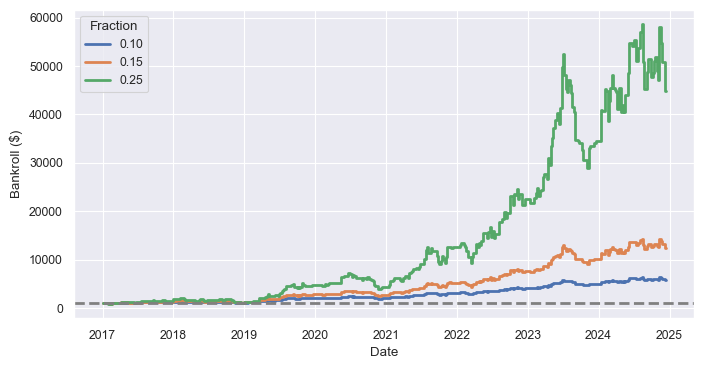
\includegraphics[width=\linewidth]{figures/bankroll_lr_case_study_simultaneous.png}
  \caption{Bankroll over time by Kelly fraction}
\end{subfigure}%
\begin{subfigure}{.5\linewidth}
  \centering
  \includegraphics[width=\linewidth]{figures/bankroll_comparison.png}
  \caption{Comparison for $f = 0.10$}
\end{subfigure}
\begin{subfigure}{.7\linewidth}
  \centering
  \includegraphics[width=\linewidth]{figures/mc_results_case_study.png}
  \caption{Simulated profit vs. observed, $f = 0.10$}
\end{subfigure}
\caption{Selection of betting performance plots}
\end{figure}

Interestingly, we see that for all fractions we place almost 1000 bets and consider more than 40\% of bouts as betting opportunities, rendering our initial concerns about sample size irrelevant. While the wider gap between our model's performance and that of the sportsbook is likely the main reason for this, computation and numerical stability may also play a role. In particular, the returns matrix and estimates of joint probabilities have much smaller dimensionalities because of the reduction in fights being considered for each event. We noticed in the original experiments that CVXPY would throw errors likely related to floating point precision more frequently, which we handled by defaulting to not betting on the event at all. With less of these cases in the fight subset experiment, we obtained nontrivial solutions for the allocation $b$ more consistently.

To close this section, it is important to acknowledge a valid concern: by filtering for fight types where the model performed well in the original experiments, we risk overfitting to the backtest data. In essence, this selection may have inadvertently tailored the dataset to highlight the model's strengths, potentially inflating the observed performance metrics. Therefore, while these results are promising, it remains to be seen whether this edge will hold up in future, unseen data. A natural and necessary next step is to track and evaluate out-of-sample performance prospectively as new fights occur. This ongoing validation will be critical in determining whether the model’s apparent edge is genuine and persistent or a byproduct of backtest optimization.



\chapter{Discussion}

This chapter reflects on the broader implications of the research, tying together the main results while considering their significance and limitations. The goal is to critically assess the performance and robustness of the modeling and betting framework developed throughout the thesis, while acknowledging the constraints and assumptions that shaped the analysis. In doing so, we also highlight the role and potential of alternative data signals, which played a key part in enriching the feature set beyond traditional sources like UFC Stats. In addition, this chapter outlines several avenues for future work that could extend or refine the current approach, particularly as new data becomes available. The chapter concludes with a summary of the contributions and the practical relevance of the findings.

\section{Key Findings}

The results of this study demonstrate that it is indeed possible to build predictive models that outperform the market in both forecast accuracy and betting profitability, particularly when leveraging a wide range of alternative data sources. Across an 8-year backtest covering nearly 4000 fights, the best-performing configuration---logistic regression with a classic Kelly staking strategy---achieved a yield of over 6\%, along with a superior log loss relative to sportsbook-implied probabilities. These findings held even under strict out-of-sample conditions, with models retrained after every event using only past data, reflecting a realistic deployment scenario.

A consistent pattern across experiments was the importance of including market-derived features. Removing the opening odds-based feature dramatically worsened both predictive accuracy and betting outcomes, reinforcing the notion that while machine learning models can surface unique signals, incorporating market sentiment remains essential. Additionally, model and strategy combinations that incorporated Venn-Abers predictors and the distributional robust Kelly strategy tended to make more conservative and targeted bets, leading to better yield and reduced drawdowns even when profit was lower in absolute terms.

The case study analysis further strengthened these conclusions. By filtering out fights involving debuting fighters and women's bouts where data is sparse or matchups are harder to evaluate, the model's relative performance improved significantly. Notably, the model’s edge over the sportsbook became much more pronounced in terms of log loss, Brier score, realized profit, and betting efficiency. This suggests that model-driven betting strategies can be most effective when carefully scoped to fight contexts where historical information is rich and stable.

Taken together, these findings support a broader message: while beating the market consistently is difficult, there are still inefficiencies to be found, especially when using information that others ignore, and when strategies are deployed selectively and evaluated rigorously.

\section{Limitations}

One key limitation of this work lies in the feature engineering and feature selection process. While we generated a large and diverse set of candidate features using domain knowledge and time-aware aggregation techniques, the approach was largely heuristic and semi-systematic. We relied on simple transformations like cumulative averages and differences without deeply exploring interaction terms or higher-order compositions. Additionally, feature selection was performed using mutual information filtering prior to modeling, which, while effective for dimensionality reduction, does not account for downstream model interactions or multicollinearity. As a result, it is likely that some useful features were excluded or underutilized, and others retained despite offering limited marginal value.

Next, only a restricted set of models and learning strategies we considered. The analysis primarily focused on logistic regression and gradient boosting as base models, with calibration added via Venn-Abers predictors. While these are strong baselines, we did not explore more advanced modeling techniques such as ensembling, stacking, or blending which may have yielded better predictive performance or more stable probability estimates.

Moreover, one of the more glaring issues in our approach comes in the form of practicality. While we have demonstrated that integrating a wide range of external data sources can significantly enhance model performance, this comes at the cost of increased complexity and fragility in the data pipeline. Relying on multiple third-party sites introduces numerous moving parts and interdependencies, making the system more difficult to maintain over time. Common issues include inconsistent data quality, changes in website structure (e.g., HTML layouts), shifting or deprecated APIs, and even the possibility of sources being taken offline altogether. Moreover, maintaining these pipelines in a live setting would be extremely challenging for a single individual, especially without strong data engineering expertise. In practice, doing so reliably would likely require a small team or substantial infrastructure to automate data ingestion, monitoring, and exception handling. On top of that, a considerable amount of manual effort was required to clean and match fighter, event, and bout identifiers across sources. While some of this logic could theoretically be automated, the sheer number of edge cases makes this a daunting task to handle algorithmically at scale. As a result, despite its potential, this multi-source approach introduces significant practical barriers to long-term deployment.

Lastly, even if such an approach was indeed profitable and able to be scaled to production levels, many sportsbooks would eventually identify the user as a sharp bettor and limit their account, typically by setting a restrictive cap on the maximum bet size. One would either need to distribute their capital across multiple sportsbooks behind shell accounts or bet on an exchange like Pinnacle which does not limit bettors at the cost of competing with even sharper lines. Since we found some evidence that suggests sportsbooks may be improving over time, this would force the user to be constantly monitoring betting performance and innovating ahead of time.

\section{Future Work}

One of the most immediate areas for future work involves addressing the practical challenges posed by the complexity of the data pipeline. A promising direction would be to perform targeted ablation studies to identify which sources and features contribute meaningfully to model performance and which can be safely discarded. By prioritizing features that are both highly predictive and reliable to maintain, we can reduce the system’s fragility. This evaluation should consider not just predictive value, but also scraping difficulty, site stability (e.g., how often its structure changes), and longevity (how long the site has been live and actively updated). Such an analysis would allow us to streamline the pipeline by eliminating high-maintenance or low-impact sources, making the system more maintainable in a live environment without significantly compromising performance.

In addition to refining the data infrastructure, another key direction is rigorous forward testing. While our backtesting framework was carefully designed to simulate realistic betting scenarios, there is always a risk of overfitting to historical quirks. To properly evaluate the durability of the model's edge, we should monitor its performance on a rolling basis as new fights occur, placing model-driven bets (even in simulation) and comparing profitability and calibration against the market in real time. This form of live or semi-live validation would provide a more reliable signal of generalization and ensure that the observed edge is not an artifact of past data, but a persistent and exploitable inefficiency.

Most importantly, while exploring more complex model architectures could yield incremental performance gains, the most substantial improvements are likely to come from enhanced feature engineering and selection. For instance, drawing inspiration from McInerney's work \citep{mcinerney_mmaai}, we could implement techniques such as time-weighted averages, Bayesian smoothing, and adjusted performance metrics that account for opponents' previous opponents to develop more nuanced features that capture the intricacies of fighter performance. We could also take on a more deliberate strategy than our ``kitchen sink" approach through manual crafting and carefully checking each candidate feature's relationship with the target as well as other features. Alternatively, on the other end of the spectrum one could extend the ``kitchen sink" approach and utilize genetic algorithms to automatically discover complicated feature combinations from our existing candidate features, drawing inspiration from Hudson River Trading's signal architecture search, which evolves computation graphs to discover predictive signals in financial data \citep{hrt_2022, hrt_2023}. In terms of feature selection, integrating techniques such as SHAP (SHapley Additive exPlanations) values can provide insights into feature importance, guiding the refinement of our feature set. Additionally, treating feature inclusion as a hyperparameter and embedding it within the model optimization process, using Bayesian optimization or genetic algorithms, could result in more efficient and predictive feature sets.

Lastly, one can use the database we constructed to investigate other relevant questions unrelated to modeling fight outcomes or sports betting due to its diversity of information. For instance, we could investigate the effect of altitude on striking and grappling output or a fighter's ability to rehydrate and regain weight after weigh-ins on their grappling performance or likelihood of winning. In addition, one could add to the database; for example, timestamped betting odds data can in theory be scraped from FightOdds.io for more granularity, which could be analyzed for market structure, sudden changes in lines, and reactions to news.

\section{Conclusion}

This thesis set out to investigate whether it is possible to systematically beat the UFC betting market by leveraging a broader set of alternative data sources and more rigorous modeling practices. Through the construction of a large, relational database integrating data from ten different websites, we significantly expanded the information available for modeling---over 50 times the size of UFC Stats alone. On top of this foundation, we explored various modeling pipelines, feature selection methods, calibration techniques, and bet sizing strategies, all validated through a realistic 8-year backtest designed to mirror real-world betting conditions.

While the results suggest that some combinations, particularly logistic regression paired with a classic Kelly strategy, can outperform market-implied probabilities and generate long-term profit, the broader takeaway is more nuanced. The difficulty in achieving statistical significance across most configurations, coupled with deteriorating performance in recent years, highlights just how efficient the market has become. Nonetheless, our work demonstrates that by incorporating unconventional data streams and rigorously evaluating strategies, it is still possible to find pockets of edge. Ultimately, this study contributes a more transparent, data-rich, and methodologically robust approach to modeling in MMA, and invites future work to build on this foundation.




\appendix
\chapter{Further Details on Database Design}

This appendix provides a comprehensive breakdown of the database structure, detailing each table and its corresponding columns. For each table, a data dictionary is included to describe the purpose, data types, and relationships between fields. This section ensures full transparency in how fight data, fighter statistics, betting odds, and other relevant information are stored and organized, supporting the reproducibility and interpretability of the analysis.


\section{Table Metadata}

\tiny
\begin{longtable}{llrrl} 
\caption{Metadata for all 58 tables in the database}\\
\toprule
Name                                    & Source          & \# Rows & \# Columns & Description                                            \endfirsthead 
\toprule
BOUT\_MAPPING                           & Multiple        & 7982    & 6          & Cross-source matching for bout IDs, UFC only                     \\
EVENT\_MAPPING                          & Multiple        & 716     & 10         & Cross-source matching for event IDs, UFC only                    \\
FIGHTER\_MAPPING                        & Multiple        & 2553    & 9          & Cross-source matching for fighter IDs, UFC only                  \\
bestfightodds\_bout\_proposition\_odds  & Best Fight Odds & 446562  & 7          & Closing odds for bout-level proposition bets           \\
bestfightodds\_event\_proposition\_odds & Best Fight Odds & 34594   & 5          & Closing odds for event-level proposition bets          \\
bestfightodds\_events                   & Best Fight Odds & 422     & 2          & Event information                                      \\
bestfightodds\_fighters                 & Best Fight Odds & 2288    & 3          & Fighter information                                    \\
bestfightodds\_moneyline\_odds          & Best Fight Odds & 2368802 & 5          & Timestamped moneyline odds by sportsbook      \\
betmma\_bouts                           & Bet MMA         & 13163   & 5          & Bout information                                       \\
betmma\_events                          & Bet MMA         & 1685    & 5          & Event information                                      \\
betmma\_fighter\_histories              & Bet MMA         & 26224   & 10         & Fighters' bout histories                               \\
betmma\_fighters                        & Bet MMA         & 7318    & 6          & Fighter information                                    \\
betmma\_late\_replacements              & Bet MMA         & 586     & 3          & Information on late replacement fighters               \\
betmma\_missed\_weights                 & Bet MMA         & 271     & 3          & Information on fighters who missed weight              \\
espn\_bout\_stats                       & ESPN            & 38610   & 33         & Bout-level striking and grappling statistics           \\
espn\_bouts                             & ESPN            & 7982    & 7          & Bout information                                       \\
espn\_events                            & ESPN            & 716     & 5          & Event information                                      \\
espn\_fighter\_histories                & ESPN            & 86730   & 14         & Fighters' bout histories                               \\
espn\_fighters                          & ESPN            & 8893    & 10         & Fighter information                                    \\
espn\_teams                             & ESPN            & 918     & 2          & Team affiliation information                           \\
espn\_venues                            & ESPN            & 223     & 6          & Venue information                                      \\
fightmatrix\_bouts                      & Fight Matrix    & 349554  & 21         & Bout information                                       \\
fightmatrix\_events                     & Fight Matrix    & 57408   & 6          & Event information                                      \\
fightmatrix\_fighter\_histories         & Fight Matrix    & 666556  & 20         & Fighters' bout histories                               \\
fightmatrix\_fighters                   & Fight Matrix    & 143615  & 4          & Fighter information                                    \\
fightmatrix\_rankings                   & Fight Matrix    & 617826  & 5          & Monthly rankings snapshots                             \\
fightoddsio\_bouts                      & FightOdds.io    & 7981    & 16         & Bout information                                       \\
fightoddsio\_events                     & FightOdds.io    & 716     & 7          & Event information                                      \\
fightoddsio\_fighters                   & FightOdds.io    & 2553    & 12         & Fighter information                                    \\
fightoddsio\_moneyline\_odds            & FightOdds.io    & 52582   & 13         & Opening/closing moneyline odds by sportsbook  \\
fightoddsio\_proposition\_odds          & FightOdds.io    & 310295  & 7          & Closing odds for proposition bets                      \\
fightoddsio\_sportsbooks                & FightOdds.io    & 18      & 5          & Sportsbook information                                 \\
mmadecisions\_bouts                     & MMA Decisions   & 6867    & 10         & Bout information                                       \\
mmadecisions\_deductions                & MMA Decisions   & 198     & 5          & Information on per-round point deductions              \\
mmadecisions\_events                    & MMA Decisions   & 1455    & 6          & Event information                                      \\
mmadecisions\_fighters                  & MMA Decisions   & 4376    & 7          & Fighter information                                    \\
mmadecisions\_judge\_scores             & MMA Decisions   & 84849   & 6          & Per-round and total scores by judge                    \\
mmadecisions\_judges                    & MMA Decisions   & 716     & 2          & Judge information                                      \\
mmadecisions\_media\_scores             & MMA Decisions   & 52630   & 6          & Opinionated total scores reported by media outlets     \\
sherdog\_bouts                          & Sherdog         & 443996  & 14         & Bout information                                       \\
sherdog\_events                         & Sherdog         & 55375   & 6          & Event information                                      \\
sherdog\_fighter\_histories             & Sherdog         & 652043  & 11         & Fighters' bout histories                               \\
sherdog\_fighters                       & Sherdog         & 140957  & 7          & Fighter information                                    \\
tapology\_bouts                         & Tapology        & 7982    & 14         & Bout information                                       \\
tapology\_community\_picks              & Tapology        & 13034   & 7          & Community predictions on bout outcomes                 \\
tapology\_events                        & Tapology        & 716     & 3          & Event information                                      \\
tapology\_fighter\_gyms                 & Tapology        & 16552   & 5          & Fighters' gym affiliations by bout                     \\
tapology\_fighter\_histories            & Tapology        & 62193   & 21         & Fighters' bout histories                               \\
tapology\_fighters                      & Tapology        & 2553    & 10         & Fighter information                                    \\
tapology\_gyms                          & Tapology        & 1056    & 5          & Gym information                                        \\
tapology\_rehydration\_weights          & Tapology        & 170     & 5          & Information on fighters' weights after rehydrating     \\
ufcstats\_bouts                         & UFC Stats       & 10483   & 16         & Bout information                                       \\
ufcstats\_events                        & UFC Stats       & 1174    & 5          & Event information                                      \\
ufcstats\_fighter\_histories            & UFC Stats       & 20966   & 4          & Fighters' bout histories                               \\
ufcstats\_fighters                      & UFC Stats       & 3862    & 7          & Fighter information                                    \\
ufcstats\_round\_stats                  & UFC Stats       & 45812   & 26         & Round-level striking and grappling statistics          \\
wikipedia\_events                       & Wikipedia       & 716     & 6          & Event information                                      \\
wikipedia\_venues                       & Wikipedia       & 214     & 6          & Venue information                                      \\
\bottomrule
\end{longtable}
\normalsize

\section{Data Dictionaries}

Data dictionaries will be organized by table source or purpose. Foreign key references will be reported in [table name].[column] form. Only ``true" foreign key relationships will be included, but all logically sound pairings can be used for table joins as long as the user is aware that incomplete records will exist in the result.

\subsection{Cross-Source Mapping Tables}

\tiny
\begin{longtable}{lllll}
\caption{Data dictionary for ``BOUT\_MAPPING" table}\\ 
\toprule
Column           & Data Type & Primary Key & Foreign Key Reference  & Description                          \endfirsthead 
\toprule
ufcstats\_id     & VARCHAR   & Yes         & ufcstats\_bouts.id     & UFC Stats bout ID                    \\
betmma\_id       & INTEGER   & No          & betmma\_bouts.id       & Corresponding Bet MMA bout ID        \\
espn\_id         & INTEGER   & No          & espn\_bouts.id         & Corresponding ESPN bout ID           \\
fightoddsio\_id  & VARCHAR   & No          & fightoddsio\_bouts.id  & Corresponding FightOdds.io bout ID   \\
mmadecisions\_id & INTEGER   & No          & mmadecisions\_bouts.id & Corresponding MMA Decisions bout ID  \\
tapology\_id     & VARCHAR   & No          & tapology\_bouts.id     & Corresponding Tapology bout ID       \\
\bottomrule
\end{longtable}
\normalsize

\newpage
\tiny
\begin{longtable}{lllll}
\caption{Data dictionary for ``EVENT\_MAPPING" table}\\ 
\toprule
Column            & Data Type & Primary Key & Foreign Key Reference    & Description                             \endfirsthead 
\toprule
ufcstats\_id      & VARCHAR   & Yes         & ufcstats\_events.id      & UFC Stats event ID                      \\
bestfightodds\_id & INTEGER   & No          & bestfightodds\_events.id & Corresponding Best Fight Odds event ID  \\
betmma\_id        & INTEGER   & No          & betmma\_events.id        & Corresponding Bet MMA event ID          \\
espn\_id          & INTEGER   & No          & espn\_events.id          & Corresponding ESPN event ID             \\
fightmatrix\_id   & INTEGER   & No          & fightmatrix\_events.id   & Corresponding Fight Matrix event ID     \\
fightoddsio\_id   & VARCHAR   & No          & fightoddsio\_events.id   & Corresponding FightOdds.io event ID     \\
mmadecisions\_id  & INTEGER   & No          & mmadecisions\_events.id  & Corresponding MMA Decisions event ID    \\
sherdog\_id       & INTEGER   & No          & sherdog\_events.id       & Corresponding Sherdog event ID          \\
tapology\_id      & VARCHAR   & No          & tapology\_events.id      & Corresponding Tapology event ID         \\
wikipedia\_id     & INTEGER   & No          & wikipedia\_events.id     & Corresponding Wikipedia event ID        \\
\bottomrule
\end{longtable}
\normalsize


\tiny
\begin{longtable}{lllll}
\caption{Data dictionary for ``FIGHTER\_MAPPING" table}\\ 
\toprule
Column            & Data Type & Primary Key & Foreign Key Reference      & Description                               \endfirsthead 
\toprule
ufcstats\_id      & VARCHAR   & Yes         & ufcstats\_fighters.id      & UFC Stats fighter ID                      \\
bestfightodds\_id & INTEGER   & No          & bestfightodds\_fighters.id & Corresponding Best Fight Odds fighter ID  \\
betmma\_id        & INTEGER   & No          & betmma\_fighters.id        & Corresponding Bet MMA fighter ID          \\
espn\_id          & INTEGER   & No          & espn\_fighters.id          & Corresponding ESPN fighter ID             \\
fightmatrix\_id   & INTEGER   & No          & fightmatrix\_fighters.id   & Corresponding Fight Matrix fighter ID     \\
fightoddsio\_id   & VARCHAR   & No          & fightoddsio\_fighters.id   & Corresponding FightOdds.io fighter ID     \\
mmadecisions\_id  & INTEGER   & No          & mmadecisions\_fighters.id  & Corresponding MMA Decisions fighter ID    \\
sherdog\_id       & INTEGER   & No          & sherdog\_fighters.id       & Corresponding Sherdog fighter ID          \\
tapology\_id      & VARCHAR   & No          & tapology\_fighters.id      & Corresponding Tapology fighter ID         \\
\bottomrule
\end{longtable}
\normalsize

\subsection{Best Fight Odds Tables}

\tiny
\begin{longtable}{lllll}
\caption{Data dictionary for ``bestfightodds\_bout\_proposition\_odds" table}\\ 
\toprule
Column             & Data Type & Primary Key & Foreign Key Reference      & Description                                                                             \endfirsthead 
\toprule
tapology\_bout\_id & VARCHAR   & No          & tapology\_bouts.id         & Tapology bout ID corresponding to bet                                       \\
event\_id          & INTEGER   & No          & bestfightodds\_events.id   & Best Fight Odds event ID~corresponding to bet                               \\
fighter\_id        & INTEGER   & No          & bestfightodds\_fighters.id & Best Fight Odds fighter ID~corresponding to bet                             \\
description        & VARCHAR   & No          & N/A                        & Description of proposition bet                                                          \\
is\_not            & INTEGER   & No          & N/A                        & Indicator for side of described outcome  \\
betsite            & VARCHAR   & No          & N/A                        & Sportsbook name                                                                         \\
odds               & INTEGER   & No          & N/A                        & Closing American odds                                                                   \\
\bottomrule
\end{longtable}
\normalsize


\tiny
\begin{longtable}{lllll}
\caption{Data dictionary for ``bestfightodds\_event\_proposition\_odds" table}\\ 
\toprule
Column      & Data Type & Primary Key & Foreign Key Reference    & Description                                    \endfirsthead 
\toprule
event\_id   & INTEGER   & No          & bestfightodds\_events.id & Best Fight Odds event ID~corresponding to bet  \\
description & VARCHAR   & No          & N/A                      & Description of proposition bet                 \\
is\_not     & INTEGER   & No          & N/A                      & Indicator for side of described outcome        \\
betsite     & VARCHAR   & No          & N/A                      & Sportsbook name                                \\
odds        & INTEGER   & No          & N/A                      & Closing American odds                          \\
\bottomrule
\end{longtable}
\normalsize


\tiny
\begin{longtable}{lllll}
\caption{Data dictionary for ``bestfightodds\_events" table}\\ 
\toprule
Column & Data Type & Primary Key & Foreign Key Reference & Description    \endfirsthead 
\toprule
id     & INTEGER   & Yes         & N/A                   & Unique ID      \\
name   & VARCHAR   & No          & N/A                   & Name of event  \\
\bottomrule
\end{longtable}
\normalsize


\tiny
\begin{longtable}{lllll}
\caption{Data dictionary for ``bestfightodds\_fighters" table}\\ 
\toprule
Column   & Data Type & Primary Key & Foreign Key Reference & Description                         \endfirsthead 
\toprule
id       & INTEGER   & Yes         & N/A                   & Unique ID                           \\
name     & VARCHAR   & No          & N/A                   & Name of fighter                     \\
nickname & VARCHAR   & No          & N/A                   & Nickname of fighter  \\
\bottomrule
\end{longtable}
\normalsize

\tiny
\begin{longtable}{lllll}
\caption{Data dictionary for ``bestfightodds\_moneyline\_odds" table}\\ 
\toprule
Column      & Data Type & Primary Key & Foreign Key Reference      & Description                                      \endfirsthead 
\toprule
event\_id   & INTEGER   & No          & bestfightodds\_events.id   & Best Fight Odds event ID corresponding to bet    \\
fighter\_id & INTEGER   & No          & bestfightodds\_fighters.id & Best Fight Odds fighter ID corresponding to bet  \\
betsite     & VARCHAR   & No          & N/A                        & Sportsbook name                                  \\
timestamp   & INTEGER   & No          & N/A                        & Unix timestamp                                   \\
odds        & INTEGER   & No          & N/A                        & American odds at given timestamp                 \\
\bottomrule
\end{longtable}
\normalsize


\subsection{Bet MMA Tables}

\tiny
\begin{longtable}{lllll}
\caption{Data dictionary for ``betmma\_bouts" table}\\ 
\toprule
Column         & Data Type & Primary Key & Foreign Key Reference & Description                     \endfirsthead 
\toprule
id             & INTEGER   & Yes         & N/A                   & Unique ID                       \\
event\_id      & INTEGER   & No          & betmma\_events.id     & Corresponding event ID          \\
bout\_order    & INTEGER   & No          & N/A                   & Order of bout within its event  \\
fighter\_1\_id & INTEGER   & No          & betmma\_fighters.id   & Fighter 1's fighter ID          \\
fighter\_2\_id & INTEGER   & No          & betmma\_fighters.id   & Fighter 2's fighter ID          \\
\bottomrule
\end{longtable}
\normalsize


\tiny
\begin{longtable}{lllll}
\caption{Data dictionary for ``betmma\_events" table}\\ 
\toprule
Column         & Data Type & Primary Key & Foreign Key Reference & Description                                 \endfirsthead 
\toprule
id             & INTEGER   & Yes         & N/A                   & Unique ID                                   \\
name           & VARCHAR   & No          & N/A                   & Name of event                               \\
date           & DATE      & No          & N/A                   & Date of event                               \\
location       & VARCHAR   & No          & N/A                   & Location of event                           \\
is\_ufc\_event & INTEGER   & No          & N/A                   & Indicator for if event is in UFC promotion  \\
\bottomrule
\end{longtable}
\normalsize

\tiny
\begin{longtable}{lllll}
\caption{Data dictionary for ``betmma\_fighter\_histories" table}\\ 
\toprule
Column                    & Data Type & Primary Key & Foreign Key Reference & Description                                            \endfirsthead 
\toprule
fighter\_id               & INTEGER   & No          & betmma\_fighters.id   & Fighter ID                                             \\
order                     & INTEGER   & No          & N/A                   & Order in fighter's bout history                        \\
bout\_id                  & INTEGER   & No          & betmma\_bouts.id      & Bout ID                                                \\
opponent\_id              & INTEGER   & No          & betmma\_fighters.id   & Opponent's fighter ID                                  \\
outcome                   & VARCHAR   & No          & N/A                   & Outcome of bout with respect to fighter  \\
outcome\_method           & VARCHAR   & No          & N/A                   & Method by which outcome was achieved                   \\
end\_round                & INTEGER   & No          & N/A                   & Round at which the bout ended                          \\
end\_round\_time\_seconds & INTEGER   & No          & N/A                   & Seconds elapsed in round at which the bout ended       \\
total\_time\_seconds      & INTEGER   & No          & N/A                   & Total seconds elapsed during bout                      \\
odds                      & INTEGER   & No          & N/A                   & American moneyline odds, likely closing                \\
\bottomrule
\end{longtable}
\normalsize

\newpage
\tiny
\begin{longtable}{lllll}
\caption{Data dictionary for ``betmma\_fighters" table}\\ 
\toprule
Column         & Data Type & Primary Key & Foreign Key Reference & Description             \endfirsthead 
\toprule
id             & INTEGER   & Yes         & N/A                   & Unique ID               \\
name           & VARCHAR   & No          & N/A                   & Name of fighter         \\
height\_inches & FLOAT     & No          & N/A                   & Height in inches        \\
reach\_inches  & FLOAT     & No          & N/A                   & Reach in inches         \\
stance         & VARCHAR   & No          & N/A                   & Fighting stance         \\
nationality    & VARCHAR   & No          & N/A                   & Nationality of fighter  \\
\bottomrule
\end{longtable}
\normalsize

\tiny
\begin{longtable}{lllll}
\caption{Data dictionary for ``betmma\_late\_replacements" table}\\ 
\toprule
Column             & Data Type & Primary Key & Foreign Key Reference & Description                        \endfirsthead 
\toprule
fighter\_id        & INTEGER   & No          & betmma\_fighters.id   & Fighter ID                         \\
bout\_id           & INTEGER   & No          & betmma\_bouts.id      & Bout ID                            \\
notice\_time\_days & INTEGER   & No          & N/A                   & Number of days notice before bout  \\
\bottomrule
\end{longtable}
\normalsize

\tiny 
\begin{longtable}{lllll}
\caption{Data dictionary for ``betmma\_missed\_weights" table}\\ 
\toprule
Column      & Data Type & Primary Key & Foreign Key Reference & Description                \endfirsthead 
\toprule
fighter\_id & INTEGER   & No          & betmma\_fighters.id   & Fighter ID                 \\
bout\_id    & INTEGER   & No          & betmma\_bouts.id      & Bout ID                    \\
weight\_lbs & FLOAT     & No          & N/A                   & Weigh-in weight in pounds  \\
\bottomrule
\end{longtable}
\normalsize

\subsection{ESPN Tables}

\tiny 
\begin{longtable}{lllll}
\caption{Data dictionary for ``espn\_bout\_stats" table}\\ 
\toprule
Column                                          & Data Type & Primary Key & Foreign Key Reference & Description                                                                                              \endfirsthead 
\toprule
bout\_id                                        & INTEGER   & No          & N/A                   & Bout ID                                                                                                  \\
fighter\_id                                     & INTEGER   & No          & N/A                   & Fighter ID                                                                                               \\
knockdowns\_scored                              & INTEGER   & No          & N/A                   & Number of knockdowns scored                                                                              \\
total\_strikes\_landed                          & INTEGER   & No          & N/A                   & Number of total strikes landed                                                                           \\
total\_strikes\_attempted                       & INTEGER   & No          & N/A                   & Number of total strikes attempted                                                                        \\
takedowns\_landed                               & INTEGER   & No          & N/A                   & Number of takedowns landed                                                                               \\
takedowns\_slams\_landed                        & INTEGER   & No          & N/A                   & \begin{tabular}[c]{@{}l@{}}Number of slam takedowns \\landed\end{tabular}                                \\
takedowns\_attempted                            & INTEGER   & No          & N/A                   & Number of takedowns attempted                                                                            \\
reversals\_scored                               & INTEGER   & No          & N/A                   & \begin{tabular}[c]{@{}l@{}}Number of position reversals \\scored\end{tabular}                            \\
significant\_strikes\_distance\_head\_landed    & INTEGER   & No          & N/A                   & \begin{tabular}[c]{@{}l@{}}Number of significant strikes \\from distance to head landed\end{tabular}     \\
significant\_strikes\_distance\_head\_attempted & INTEGER   & No          & N/A                   & \begin{tabular}[c]{@{}l@{}}Number of significant strikes \\from distance to head attempted\end{tabular}  \\
significant\_strikes\_distance\_body\_landed    & INTEGER   & No          & N/A                   & \begin{tabular}[c]{@{}l@{}}Number of significant strikes \\from distance to body landed\end{tabular}     \\
significant\_strikes\_distance\_body\_attempted & INTEGER   & No          & N/A                   & \begin{tabular}[c]{@{}l@{}}Number of significant strikes \\from distance to body attempted\end{tabular}  \\
significant\_strikes\_distance\_leg\_landed     & INTEGER   & No          & N/A                   & \begin{tabular}[c]{@{}l@{}}Number of significant strikes \\from distance to leg landed\end{tabular}      \\
significant\_strikes\_distance\_leg\_attempted  & INTEGER   & No          & N/A                   & \begin{tabular}[c]{@{}l@{}}Number of significant strikes \\from distance to leg attempted\end{tabular}   \\
significant\_strikes\_clinch\_head\_landed      & INTEGER   & No          & N/A                   & \begin{tabular}[c]{@{}l@{}}Number of significant strikes \\from clinch to head landed\end{tabular}       \\
significant\_strikes\_clinch\_head\_attempted   & INTEGER   & No          & N/A                   & \begin{tabular}[c]{@{}l@{}}Number of significant strikes \\from~clinch to head attempted\end{tabular}    \\
significant\_strikes\_clinch\_body\_landed      & INTEGER   & No          & N/A                   & \begin{tabular}[c]{@{}l@{}}Number of significant strikes \\from~clinch to body landed\end{tabular}       \\
significant\_strikes\_clinch\_body\_attempted   & INTEGER   & No          & N/A                   & \begin{tabular}[c]{@{}l@{}}Number of significant strikes \\from clinch to body attempted\end{tabular}    \\
significant\_strikes\_clinch\_leg\_landed       & INTEGER   & No          & N/A                   & \begin{tabular}[c]{@{}l@{}}Number of significant strikes \\from clinch to leg landed\end{tabular}        \\
significant\_strikes\_clinch\_leg\_attempted    & INTEGER   & No          & N/A                   & \begin{tabular}[c]{@{}l@{}}Number of significant strikes \\from clinch to leg attempted\end{tabular}     \\
significant\_strikes\_ground\_head\_landed      & INTEGER   & No          & N/A                   & \begin{tabular}[c]{@{}l@{}}Number of significant strikes \\from ground to head landed\end{tabular}       \\
significant\_strikes\_ground\_head\_attempted   & INTEGER   & No          & N/A                   & \begin{tabular}[c]{@{}l@{}}Number of significant strikes \\from ground to head attempted\end{tabular}    \\
significant\_strikes\_ground\_body\_landed      & INTEGER   & No          & N/A                   & \begin{tabular}[c]{@{}l@{}}Number of significant strikes \\from ground to body landed\end{tabular}       \\
significant\_strikes\_ground\_body\_attempted   & INTEGER   & No          & N/A                   & \begin{tabular}[c]{@{}l@{}}Number of significant strikes \\from ground to body attempted\end{tabular}    \\
significant\_strikes\_ground\_leg\_landed       & INTEGER   & No          & N/A                   & \begin{tabular}[c]{@{}l@{}}Number of significant strikes \\from ground to leg landed\end{tabular}        \\
significant\_strikes\_ground\_leg\_attempted    & INTEGER   & No          & N/A                   & \begin{tabular}[c]{@{}l@{}}Number of significant strikes \\from ground to leg attempted\end{tabular}     \\
advances                                        & INTEGER   & No          & N/A                   & Number of advances                                                                                       \\
advances\_to\_back                              & INTEGER   & No          & N/A                   & \begin{tabular}[c]{@{}l@{}}Number of advances to \\back control\end{tabular}                             \\
advances\_to\_half\_guard                       & INTEGER   & No          & N/A                   & \begin{tabular}[c]{@{}l@{}}Number of advances to \\half guard\end{tabular}                               \\
advances\_to\_mount                             & INTEGER   & No          & N/A                   & Number of advances to mount                                                                              \\
advances\_to\_side                              & INTEGER   & No          & N/A                   & \begin{tabular}[c]{@{}l@{}}Number of advances to \\side control\end{tabular}                             \\
submissions\_attempted                          & INTEGER   & No          & N/A                   & \begin{tabular}[c]{@{}l@{}}Number of submissions \\attempted\end{tabular}                                \\
\bottomrule
\end{longtable}
\normalsize

\tiny 
\begin{longtable}{lllll}
\caption{Data dictionary for ``espn\_bouts" table}\\ 
\toprule
Column         & Data Type & Primary Key & Foreign Key Reference & Description                     \endfirsthead 
\toprule
id             & INTEGER   & Yes         & N/A                   & Unique ID                       \\
event\_id      & INTEGER   & No          & espn\_events.id       & Event ID                        \\
bout\_order    & INTEGER   & No          & N/A                   & Order of bout within its event  \\
fighter\_1\_id & INTEGER   & No          & espn\_fighters.id     & Fighter 1's fighter ID          \\
fighter\_2\_id & INTEGER   & No          & espn\_fighters.id     & Fighter 2's fighter ID          \\
winner\_id     & INTEGER   & No          & espn\_fighters.id     & Winner's fighter ID             \\
card\_segment  & VARCHAR   & No          & N/A                   & Section of event's fight card   \\
\bottomrule
\end{longtable}
\normalsize

\tiny 
\begin{longtable}{lllll}
\caption{Data dictionary for ``espn\_events" table}\\ 
\toprule
Column    & Data Type & Primary Key & Foreign Key Reference & Description                        \endfirsthead 
\toprule
id        & INTEGER   & Yes         & N/A                   & Unique ID                          \\
name      & VARCHAR   & No          & N/A                   & Name of event                      \\
date      & DATE      & No          & N/A                   & Date of event                      \\
hour\_utc & INTEGER   & No          & N/A                   & Hour at which event starts in UTC  \\
venue\_id & INTEGER   & No          & espn\_venues.id       & Event's venue ID                   \\
\bottomrule
\end{longtable}
\normalsize

\newpage
\tiny 
\begin{longtable}{lllll}
\caption{Data dictionary for ``espn\_fighter\_histories" table}\\ 
\toprule
Column                    & Data Type & Primary Key & Foreign Key Reference & Description                                   \endfirsthead 
\toprule
fighter\_id               & INTEGER   & No          & N/A                   & Fighter ID                                    \\
order                     & INTEGER   & No          & N/A                   & Order in fighter's bout history               \\
bout\_id                  & INTEGER   & No          & N/A                   & Bout ID                                       \\
event\_id                 & INTEGER   & No          & N/A                   & Event ID                                      \\
event\_name               & VARCHAR   & No          & N/A                   & Name of event                                 \\
date                      & DATE      & No          & N/A                   & Date of bout                                  \\
hour\_utc                 & INTEGER   & No          & N/A                   & Hour of bout in UTC                           \\
opponent\_id              & INTEGER   & No          & N/A                   & Opponent's fighter ID                         \\
outcome                   & VARCHAR   & No          & N/A                   & Outcome of bout with respect to fighter       \\
outcome\_method           & VARCHAR   & No          & N/A                   & Method by which outcome was achieved          \\
end\_round                & INTEGER   & No          & N/A                   & Round at which bout ended                     \\
end\_round\_time\_seconds & INTEGER   & No          & N/A                   & Seconds elapsed in round at which bout ended  \\
total\_time\_seconds      & INTEGER   & No          & N/A                   & Total seconds elapsed during bout             \\
is\_title\_bout           & INTEGER   & No          & N/A                   & Indicator for if the bout was a title fight   \\
\bottomrule
\end{longtable}
\normalsize

\tiny 
\begin{longtable}{lllll}
\caption{Data dictionary for ``espn\_fighters" table}\\ 
\toprule
Column          & Data Type & Primary Key & Foreign Key Reference & Description                    \endfirsthead 
\toprule
id              & INTEGER   & Yes         & N/A                   & Unique ID                      \\
name            & VARCHAR   & No          & N/A                   & Name of fighter                \\
nickname        & VARCHAR   & No          & N/A                   & Nickname of fighter            \\
date\_of\_birth & DATE      & No          & N/A                   & Date of birth                  \\
reach\_inches   & FLOAT     & No          & N/A                   & Reach in inches                \\
height\_inches  & INTEGER   & No          & N/A                   & Height in inches               \\
stance          & VARCHAR   & No          & N/A                   & Fighting stance                \\
team\_id        & INTEGER   & No          & espn\_teams.id        & Team affiliation               \\
nationality     & VARCHAR   & No          & N/A                   & Nationality of fighter         \\
fighting\_style & VARCHAR   & No          & N/A                   & Self-described fighting style  \\
\bottomrule
\end{longtable}
\normalsize

\tiny 
\begin{longtable}{lllll}
\caption{Data dictionary for ``espn\_teams" table}\\ 
\toprule
Column & Data Type & Primary Key & Foreign Key Reference & Description       \endfirsthead 
\toprule
id     & INTEGER   & Yes         & N/A                   & Unique ID         \\
name   & VARCHAR   & No          & N/A                   & Name of team/gym  \\
\bottomrule
\end{longtable}
\normalsize

\tiny 
\begin{longtable}{lllll}
\caption{Data dictionary for ``espn\_venues" table}\\ 
\toprule
Column     & Data Type & Primary Key & Foreign Key Reference & Description                        \endfirsthead 
\toprule
id         & INTEGER   & Yes         & N/A                   & Unique ID                          \\
name       & VARCHAR   & No          & N/A                   & Name of venue                      \\
city       & VARCHAR   & No          & N/A                   & City venue is located in           \\
state      & VARCHAR   & No          & N/A                   & State venue is located in          \\
country    & VARCHAR   & No          & N/A                   & Country venue is located in        \\
is\_indoor & INTEGER   & No          & N/A                   & Indicator for if venue is indoors  \\
\bottomrule
\end{longtable}
\normalsize

\newpage 
\subsection{Fight Matrix Tables}
\tiny 
\begin{longtable}{lllll}
\caption{Data dictionary for ``fightmatrix\_bouts" table}\\ 
\toprule
Column                          & Data Type & Primary Key & Foreign Key Reference  & Description                                \endfirsthead 
\toprule
event\_id                       & INTEGER   & No          & fightmatrix\_events.id & Event ID                                   \\
bout\_order                     & INTEGER   & No          & N/A                    & Order of bout within its event             \\
fighter\_1\_id                  & INTEGER   & No          & N/A                    & Fighter 1's fighter ID                     \\
fighter\_2\_id                  & INTEGER   & No          & N/A                    & Fighter 2's fighter ID                     \\
fighter\_1\_outcome             & VARCHAR   & No          & N/A                    & Fighter 1's outcome                        \\
fighter\_2\_outcome             & VARCHAR   & No          & N/A                    & Fighter 2's outcome                        \\
fighter\_1\_elo\_k170\_pre      & INTEGER   & No          & N/A                    & Fighter 1's pre-bout K = 170 Elo rating    \\
fighter\_1\_elo\_k170\_post     & INTEGER   & No          & N/A                    & Fighter 1's post-bout K = 170 Elo rating   \\
fighter\_1\_elo\_modified\_pre  & INTEGER   & No          & N/A                    & Fighter 1's pre-bout modified Elo rating   \\
fighter\_1\_elo\_modified\_post & INTEGER   & No          & N/A                    & Fighter 1's post-bout modified Elo rating  \\
fighter\_1\_glicko\_1\_pre      & INTEGER   & No          & N/A                    & Fighter 1's pre-bout Glicko-1 rating       \\
fighter\_1\_glicko\_1\_post     & INTEGER   & No          & N/A                    & Fighter 1's post-bout Glicko-1 rating      \\
fighter\_2\_elo\_k170\_pre      & INTEGER   & No          & N/A                    & Fighter 2's pre-bout K = 170 Elo rating    \\
fighter\_2\_elo\_k170\_post     & INTEGER   & No          & N/A                    & Fighter 2's post-bout K = 170 Elo rating   \\
fighter\_2\_elo\_modified\_pre  & INTEGER   & No          & N/A                    & Fighter 2's pre-bout modified Elo rating   \\
fighter\_2\_elo\_modified\_post & INTEGER   & No          & N/A                    & Fighter 2's post-bout modified Elo rating  \\
fighter\_2\_glicko\_1\_pre      & INTEGER   & No          & N/A                    & Fighter 2's pre-bout Glicko-1 rating       \\
fighter\_2\_glicko\_1\_post     & INTEGER   & No          & N/A                    & Fighter 2's post-bout Glicko-1 rating      \\
weight\_class                   & VARCHAR   & No          & N/A                    & Weight class name                          \\
outcome\_method                 & VARCHAR   & No          & N/A                    & Method by which outcome was achieved       \\
end\_round                      & INTEGER   & No          & N/A                    & Round at which bout ended                  \\
\bottomrule
\end{longtable}
\normalsize

\tiny 
\begin{longtable}{lllll}
\caption{Data dictionary for ``fightmatrix\_events" table}\\ 
\toprule
Column         & Data Type & Primary Key & Foreign Key Reference & Description                                 \endfirsthead 
\toprule
id             & INTEGER   & Yes         & N/A                   & Unique ID                                   \\
name           & VARCHAR   & No          & N/A                   & Name of event                               \\
promotion      & VARCHAR   & No          & N/A                   & Promotion in which event takes place        \\
date           & DATE      & No          & N/A                   & Date of event                               \\
country        & VARCHAR   & No          & N/A                   & Country in which event takes place          \\
is\_ufc\_event & INTEGER   & No          & N/A                   & Indicator for if event is in UFC promotion  \\
\bottomrule
\end{longtable}
\normalsize

\tiny 
\begin{longtable}{lllll}
\caption{Data dictionary for ``fightmatrix\_fighter\_histories" table}\\ 
\toprule
Column                        & Data Type & Primary Key & Foreign Key Reference  & Description                               \endfirsthead 
\toprule
fighter\_id                   & INTEGER   & No          & N/A                    & Fighter ID                                \\
order                         & INTEGER   & No          & N/A                    & Order in fighter's bout history           \\
event\_id                     & INTEGER   & No          & fightmatrix\_events.id & Event ID                                  \\
date                          & DATE      & No          & N/A                    & Date of bout                              \\
opponent\_id                  & INTEGER   & No          & N/A                    & Opponent's fighter ID                     \\
outcome                       & VARCHAR   & No          & N/A                    & Outcome of bout                           \\
outcome\_method               & VARCHAR   & No          & N/A                    & Method by which outcome was achieved      \\
end\_round                    & INTEGER   & No          & N/A                    & Round at which bout ended                 \\
fighter\_elo\_k170\_pre       & INTEGER   & No          & N/A                    & Fighter's pre-bout K = 170 Elo rating     \\
fighter\_elo\_k170\_post      & INTEGER   & No          & N/A                    & Fighter's post-bout K = 170 Elo rating    \\
fighter\_elo\_modified\_pre   & INTEGER   & No          & N/A                    & Fighter's pre-bout modified Elo rating    \\
fighter\_elo\_modified\_post  & INTEGER   & No          & N/A                    & Fighter's post-bout modified Elo rating   \\
fighter\_glicko\_1\_pre       & INTEGER   & No          & N/A                    & Fighter's pre-bout Glicko-1 rating        \\
fighter\_glicko\_1\_post      & INTEGER   & No          & N/A                    & Fighter's post-bout Glicko-1 rating       \\
opponent\_elo\_k170\_pre      & INTEGER   & No          & N/A                    & Opponent's pre-bout K = 170 Elo rating    \\
opponent\_elo\_k170\_post     & INTEGER   & No          & N/A                    & Opponent's post-bout K = 170 Elo rating   \\
opponent\_elo\_modified\_pre  & INTEGER   & No          & N/A                    & Opponent's pre-bout modified Elo rating   \\
opponent\_elo\_modified\_post & INTEGER   & No          & N/A                    & Opponent's post-bout modified Elo rating  \\
opponent\_glicko\_1\_pre      & INTEGER   & No          & N/A                    & Opponent's pre-bout Glicko-1 rating       \\
opponent\_glicko\_1\_post     & INTEGER   & No          & N/A                    & Opponent's post-bout Glicko-1 rating      \\
\bottomrule
\end{longtable}
\normalsize

\tiny 
\begin{longtable}{lllll}
\caption{Data dictionary for ``fightmatrix\_fighters" table}\\ 
\toprule
Column           & Data Type & Primary Key & Foreign Key Reference & Description                     \endfirsthead 
\toprule
id               & INTEGER   & Yes         & N/A                   & Unique ID                       \\
name             & VARCHAR   & No          & N/A                   & Name of fighter                 \\
pro\_debut\_date & DATE      & No          & N/A                   & Date of professional MMA debut  \\
ufc\_debut\_date & DATE      & No          & N/A                   & Date of UFC debut               \\
\bottomrule
\end{longtable}
\normalsize

\tiny 
\begin{longtable}{lllll}
\caption{Data dictionary for ``fightmatrix\_rankings" table}\\ 
\toprule
Column        & Data Type & Primary Key & Foreign Key Reference & Description                   \endfirsthead 
\toprule
issue\_date   & DATE      & No          & N/A                   & Publication date of rankings  \\
weight\_class & VARCHAR   & No          & N/A                   & Weight class name             \\
fighter\_id   & INTEGER   & No          & N/A                   & Fighter ID                    \\
rank          & INTEGER   & No          & N/A                   & Ordinal ranking               \\
points        & INTEGER   & No          & N/A                   & Rank-specific rating points   \\
\bottomrule
\end{longtable}
\normalsize

\subsection{FightOdds.io Tables}
\tiny 
\begin{longtable}{lllll}
\caption{Data dictionary for ``fightoddsio\_bouts" table}\\ 
\toprule
Column                   & Data Type & Primary Key & Foreign Key Reference    & Description                                       \endfirsthead 
\toprule
id                       & VARCHAR   & Yes         & N/A                      & Unique ID                                         \\
pk                       & INTEGER   & No          & N/A                      & Unique integer primary key                        \\
slug                     & VARCHAR   & No          & N/A                      & Unique slug                                       \\
event\_id                & VARCHAR   & No          & fightoddsio\_events.id   & Event ID                                          \\
fighter\_1\_id           & VARCHAR   & No          & fightoddsio\_fighters.id & Fighter 1's fighter ID                            \\
fighter\_2\_id           & VARCHAR   & No          & fightoddsio\_fighters.id & Fighter 2's fighter ID                            \\
winner\_id               & VARCHAR   & No          & fightoddsio\_fighters.id & Winner's fighter ID                               \\
bout\_type               & VARCHAR   & No          & N/A                      & Type of bout in terms of card segment             \\
weight\_class            & VARCHAR   & No          & N/A                      & Weight class name                                 \\
weight\_lbs              & INTEGER   & No          & N/A                      & Weight class's weight limit in pounds             \\
outcome\_method          & VARCHAR   & No          & N/A                      & Method of bout outcome                            \\
outcome\_method\_details & VARCHAR   & No          & N/A                      & Details on outcome method                         \\
end\_round               & INTEGER   & No          & N/A                      & Round at which bout ended                         \\
end\_round\_time         & VARCHAR   & No          & N/A                      & Time in end round in MM:SS format                 \\
fighter\_1\_odds         & INTEGER   & No          & N/A                      & Fighter 1's mean closing American moneyline odds  \\
fighter\_2\_odds         & INTEGER   & No          & N/A                      & Fighter 2's mean closing American moneyline odds  \\
\bottomrule
\end{longtable}
\normalsize

\tiny 
\begin{longtable}{lllll}
\caption{Data dictionary for ``fightoddsio\_events" table}\\ 
\toprule
Column   & Data Type & Primary Key & Foreign Key Reference & Description                 \endfirsthead 
\toprule
id       & VARCHAR   & Yes         & N/A                   & Unique ID                   \\
pk       & INTEGER   & No          & N/A                   & Unique integer primary key  \\
slug     & VARCHAR   & No          & N/A                   & Unique slug                 \\
name     & VARCHAR   & No          & N/A                   & Name of event               \\
date     & DATE      & No          & N/A                   & Date of event               \\
location & VARCHAR   & No          & N/A                   & Location of event           \\
venue    & VARCHAR   & No          & N/A                   & Name of venue               \\
\bottomrule
\end{longtable}
\normalsize

\newpage
\tiny 
\begin{longtable}{lllll}
\caption{Data dictionary for ``fightoddsio\_fighters" table}\\ 
\toprule
Column              & Data Type & Primary Key & Foreign Key Reference & Description                  \endfirsthead 
\toprule
id                  & VARCHAR   & Yes         & N/A                   & Unique ID                    \\
pk                  & INTEGER   & No          & N/A                   & Unique integer primary key   \\
slug                & VARCHAR   & No          & N/A                   & Unique slug                  \\
name                & VARCHAR   & No          & N/A                   & Name of fighter              \\
nickname            & VARCHAR   & No          & N/A                   & Nickname of fighter          \\
date\_of\_birth     & DATE      & No          & N/A                   & Date of birth                \\
height\_centimeters & FLOAT     & No          & N/A                   & Height in centimeters        \\
reach\_inches       & FLOAT     & No          & N/A                   & Reach in inches              \\
leg\_reach\_inches  & INTEGER   & No          & N/A                   & Leg reach in inches          \\
fighting\_style     & VARCHAR   & No          & N/A                   & Standardized fighting style  \\
stance              & VARCHAR   & No          & N/A                   & Fighting stance              \\
nationality         & VARCHAR   & No          & N/A                   & Nationality of fighter       \\
\bottomrule
\end{longtable}
\normalsize

\tiny 
\begin{longtable}{lllll}
\caption{Data dictionary for ``fightoddsio\_moneyline\_odds" table}\\ 
\toprule
Column                    & Data Type & Primary Key & Foreign Key Reference       & Description                        \endfirsthead 
\toprule
id                        & VARCHAR   & Yes         & N/A                         & Unique ID                          \\
bout\_id                  & VARCHAR   & No          & fightoddsio\_bouts.id       & Bout ID                            \\
sportsbook\_id            & VARCHAR   & No          & fightoddsio\_sportsbooks.id & Sportsbook ID                      \\
outcome\_1\_id            & VARCHAR   & No          & N/A                         & Outcome ID for fighter 1 winning   \\
fighter\_1\_odds\_open    & INTEGER   & No          & N/A                         & Fighter 1's opening American odds  \\
fighter\_1\_odds\_worst   & INTEGER   & No          & N/A                         & Fighter 1's worst American odds    \\
fighter\_1\_odds\_current & INTEGER   & No          & N/A                         & Fighter 1's latest American odds   \\
fighter\_1\_odds\_best    & INTEGER   & No          & N/A                         & Fighter 1's best American odds     \\
outcome\_2\_id            & VARCHAR   & No          & N/A                         & Outcome ID for fighter 2 winning   \\
fighter\_2\_odds\_open    & INTEGER   & No          & N/A                         & Fighter 2's opening American odds  \\
fighter\_2\_odds\_worst   & INTEGER   & No          & N/A                         & Fighter 2's worst American odds    \\
fighter\_2\_odds\_current & INTEGER   & No          & N/A                         & Fighter 2's latest American odds   \\
fighter\_2\_odds\_best    & INTEGER   & No          & N/A                         & Fighter 2's best American odds     \\
\bottomrule
\end{longtable}
\normalsize

\tiny 
\begin{longtable}{lllll}
\caption{Data dictionary for ``fightoddsio\_proposition\_odds" table}\\ 
\toprule
Column           & Data Type & Primary Key & Foreign Key Reference & Description                              \endfirsthead 
\toprule
bout\_id         & VARCHAR   & No          & N/A                   & Bout ID                                  \\
offer\_type\_id  & VARCHAR   & No          & N/A                   & Standardized offer type                  \\
is\_not          & INTEGER   & No          & N/A                   & Indicator for side of bet                \\
average\_odds    & INTEGER   & No          & N/A                   & Average American odds                    \\
fighter\_pk      & INTEGER   & No          & N/A                   & Primary key of fighter being referenced  \\
description      & VARCHAR   & No          & N/A                   & Description of proposition bet           \\
not\_description & VARCHAR   & No          & N/A                   & Description of opposing side of bet      \\
\bottomrule
\end{longtable}
\normalsize

\tiny 
\begin{longtable}{lllll}
\caption{Data dictionary for ``fightoddsio\_sportsbooks" table}\\ 
\toprule
Column       & Data Type & Primary Key & Foreign Key Reference & Description                               \endfirsthead 
\toprule
id           & VARCHAR   & Yes         & N/A                   & Unique ID                                 \\
slug         & VARCHAR   & No          & N/A                   & Unique slug                               \\
short\_name  & VARCHAR   & No          & N/A                   & Abbreviated or common name of sportsbook  \\
full\_name   & VARCHAR   & No          & N/A                   & Full name of sportsbook                   \\
website\_url & VARCHAR   & No          & N/A                   & Website URL of sportsbook                 \\
\bottomrule
\end{longtable}
\normalsize

\newpage
\subsection{MMA Decisions Tables}
\tiny 
\begin{longtable}{lllll}
\caption{Data dictionary for ``mmadecisions\_bouts" table}\\ 
\toprule
Column                        & Data Type & Primary Key & Foreign Key Reference     & Description                            \endfirsthead 
\toprule
id                            & INTEGER   & Yes         & N/A                       & Unique ID                              \\
event\_id                     & INTEGER   & No          & mmadecisions\_events.id   & Event ID                               \\
bout\_order                   & INTEGER   & No          & N/A                       & Order of bout within its event         \\
fighter\_1\_id                & INTEGER   & No          & mmadecisions\_fighters.id & Fighter 1's fighter ID                 \\
fighter\_2\_id                & INTEGER   & No          & mmadecisions\_fighters.id & Fighter 2's fighter ID                 \\
fighter\_1\_weight\_lbs       & FLOAT     & No          & N/A                       & Fighter 1's weigh-in result in pounds  \\
fighter\_2\_weight\_lbs       & FLOAT     & No          & N/A                       & Fighter 2's weigh-in result in pounds  \\
fighter\_1\_fighting\_out\_of & VARCHAR   & No          & N/A                       & Location fighter 1 is fighting out of  \\
fighter\_2\_fighting\_out\_of & VARCHAR   & No          & N/A                       & Location fighter 2 is fighting out of  \\
decision\_type                & VARCHAR   & No          & N/A                       & Type of decision made, e.g. unanimous  \\
\bottomrule
\end{longtable}
\normalsize


\tiny 
\begin{longtable}{lllll}
\caption{Data dictionary for ``mmadecisions\_deductions" table}\\ 
\toprule
Column           & Data Type & Primary Key & Foreign Key Reference     & Description                                    \endfirsthead 
\toprule
bout\_id         & INTEGER   & No          & mmadecisions\_bouts.id    & Bout ID                                        \\
fighter\_id      & INTEGER   & No          & mmadecisions\_fighters.id & Fighter ID                                     \\
round\_number    & INTEGER   & No          & N/A                       & Round in which points were deducted            \\
points\_deducted & INTEGER   & No          & N/A                       & Number of points deducted from all scorecards  \\
reason           & VARCHAR   & No          & N/A                       & Reason for deduction                           \\
\bottomrule
\end{longtable}
\normalsize

\tiny 
\begin{longtable}{lllll}
\caption{Data dictionary for ``mmadecisions\_events" table}\\ 
\toprule
Column    & Data Type & Primary Key & Foreign Key Reference & Description                            \endfirsthead 
\toprule
id        & INTEGER   & Yes         & N/A                   & Unique ID                              \\
name      & VARCHAR   & No          & N/A                   & Name of event                          \\
promotion & VARCHAR   & No          & N/A                   & Promotion in which events takes place  \\
date      & DATE      & No          & N/A                   & Date of event                          \\
venue     & VARCHAR   & No          & N/A                   & Name of venue                          \\
location  & VARCHAR   & No          & N/A                   & Location of event                      \\
\bottomrule
\end{longtable}
\normalsize

\tiny 
\begin{longtable}{lllll}
\caption{Data dictionary for ``mmadecisions\_fighters" table}\\ 
\toprule
Column          & Data Type & Primary Key & Foreign Key Reference & Description                      \endfirsthead 
\toprule
id              & INTEGER   & Yes         & N/A                   & Unique ID                        \\
name            & VARCHAR   & No          & N/A                   & Name of fighter                  \\
nicknames       & VARCHAR   & No          & N/A                   & Nickname(s) of fighter           \\
date\_of\_birth & DATE      & No          & N/A                   & Date of birth                    \\
birth\_location & VARCHAR   & No          & N/A                   & Location where fighter was born  \\
height\_inches  & FLOAT     & No          & N/A                   & Height in inches                 \\
reach\_inches   & FLOAT     & No          & N/A                   & Reach in inches                  \\
\bottomrule
\end{longtable}
\normalsize

\tiny 
\begin{longtable}{lllll}
\caption{Data dictionary for ``mmadecisions\_judge\_scores" table}\\ 
\toprule
Column            & Data Type & Primary Key & Foreign Key Reference   & Description                     \endfirsthead 
\toprule
bout\_id          & INTEGER   & No          & mmadecisions\_bouts.id  & Bout ID                         \\
round             & VARCHAR   & No          & N/A                     & Round number or ``Total"  \\
judge\_id         & INTEGER   & No          & mmadecisions\_judges.id & Judge ID                        \\
judge\_order      & INTEGER   & No          & N/A                     & Order within judges             \\
fighter\_1\_score & INTEGER   & No          & N/A                     & Fighter 1's score               \\
fighter\_2\_score & INTEGER   & No          & N/A                     & Fighter 2's score               \\
\bottomrule
\end{longtable}
\normalsize

\newpage 
\tiny
\begin{longtable}{lllll}
\caption{Data dictionary for ``mmadecisions\_judges" table}\\ 
\toprule
Column & Data Type & Primary Key & Foreign Key Reference & Description    \endfirsthead 
\toprule
id     & INTEGER   & Yes         & N/A                   & Unique ID      \\
name   & VARCHAR   & No          & N/A                   & Name of judge  \\
\bottomrule
\end{longtable}
\normalsize

\tiny 
\begin{longtable}{lllll}
\caption{Data dictionary for ``mmadecisions\_media\_scores" table}\\ 
\toprule
Column            & Data Type & Primary Key & Foreign Key Reference  & Description                            \endfirsthead 
\toprule
bout\_id          & INTEGER   & No          & mmadecisions\_bouts.id & Bout ID                                \\
person\_name      & VARCHAR   & No          & N/A                    & Name of media outlet's representative  \\
media\_name       & VARCHAR   & No          & N/A                    & Name of media outlet                   \\
fighter\_1\_score & INTEGER   & No          & N/A                    & Fighter 1's media score                \\
fighter\_2\_score & INTEGER   & No          & N/A                    & Fighter 2's media score                \\
order             & INTEGER   & No          & N/A                    & Order within media scores              \\
\bottomrule
\end{longtable}
\normalsize

\subsection{Sherdog Tables}
\tiny 
\begin{longtable}{lllll}
\caption{Data dictionary for ``sherdog\_bouts" table}\\ 
\toprule
Column                    & Data Type & Primary Key & Foreign Key Reference & Description                                     \endfirsthead 
\toprule
event\_id                 & INTEGER   & No          & sherdog\_events.id    & Event ID                                        \\
bout\_order               & INTEGER   & No          & N/A                   & Order of bout within its event                  \\
fighter\_1\_id            & INTEGER   & No          & N/A                   & Fighter 1's fighter ID                          \\
fighter\_2\_id            & INTEGER   & No          & N/A                   & Fighter 2's fighter ID                          \\
fighter\_1\_outcome       & VARCHAR   & No          & N/A                   & Fighter 1's outcome                             \\
fighter\_2\_outcome       & VARCHAR   & No          & N/A                   & Fighter 2's outcome                             \\
is\_title\_bout           & INTEGER   & No          & N/A                   & Indicator for if bout is a title fight          \\
weight\_class             & VARCHAR   & No          & N/A                   & Name of weight class                            \\
weight\_class\_lbs        & INTEGER   & No          & N/A                   & Weight in pounds corresponding to weight class  \\
outcome\_method           & VARCHAR   & No          & N/A                   & Method by which outcome was achieved            \\
outcome\_method\_broad    & VARCHAR   & No          & N/A                   & Broad categorization of outcome method          \\
end\_round                & INTEGER   & No          & N/A                   & Round at which bout ended                       \\
end\_round\_time\_seconds & INTEGER   & No          & N/A                   & Seconds elapsed in round at which bout ended    \\
total\_time\_seconds      & INTEGER   & No          & N/A                   & Total seconds elapsed during bout               \\
\bottomrule
\end{longtable}
\normalsize

\tiny 
\begin{longtable}{lllll}
\caption{Data dictionary for ``sherdog\_events" table}\\ 
\toprule
Column         & Data Type & Primary Key & Foreign Key Reference & Description                                 \endfirsthead 
\toprule
id             & INTEGER   & Yes         & N/A                   & Unique ID                                   \\
name           & VARCHAR   & No          & N/A                   & Name of event                               \\
date           & DATE      & No          & N/A                   & Date of event                               \\
location       & VARCHAR   & No          & N/A                   & Location event takes place in               \\
country        & VARCHAR   & No          & N/A                   & Country event takes place in                \\
is\_ufc\_event & INTEGER   & No          & N/A                   & Indicator for if event is in UFC promotion  \\
\bottomrule
\end{longtable}
\normalsize

\newpage
\tiny 
\begin{longtable}{lllll}
\caption{Data dictionary for ``sherdog\_fighter\_histories" table}\\ 
\toprule
Column                    & Data Type & Primary Key & Foreign Key Reference & Description                                   \endfirsthead 
\toprule
fighter\_id               & INTEGER   & No          & sherdog\_fighters.id  & Fighter ID                                    \\
order                     & INTEGER   & No          & N/A                   & Order in fighter's bout history               \\
event\_id                 & INTEGER   & No          & sherdog\_events.id    & Event ID                                      \\
date                      & DATE      & No          & N/A                   & Date of bout                                  \\
opponent\_id              & INTEGER   & No          & sherdog\_fighters.id  & Opponent's fighter ID                         \\
outcome                   & VARCHAR   & No          & N/A                   & Outcome of bout                               \\
outcome\_method           & VARCHAR   & No          & N/A                   & Method by which outcome was achieved          \\
outcome\_method\_broad    & VARCHAR   & No          & N/A                   & Broad categorization of outcome method        \\
end\_round                & INTEGER   & No          & N/A                   & Round at which bout ended                     \\
end\_round\_time\_seconds & INTEGER   & No          & N/A                   & Seconds elapsed in round at which bout ended  \\
total\_time\_seconds      & INTEGER   & No          & N/A                   & Total seconds elapsed during bout             \\
\bottomrule
\end{longtable}
\normalsize

\tiny 
\begin{longtable}{lllll}
\caption{Data dictionary for ``sherdog\_fighters" table}\\ 
\toprule
Column           & Data Type & Primary Key & Foreign Key Reference & Description                     \endfirsthead 
\toprule
id               & INTEGER   & Yes         & N/A                   & Unique ID                       \\
name             & VARCHAR   & No          & N/A                   & Name of fighter                 \\
nickname         & VARCHAR   & No          & N/A                   & Nickname of fighter             \\
height\_inches   & INTEGER   & No          & N/A                   & Height in inches                \\
date\_of\_birth  & DATE      & No          & N/A                   & Date of birth                   \\
nationality      & VARCHAR   & No          & N/A                   & Nationality of fighter          \\
pro\_debut\_date & DATE      & No          & N/A                   & Date of professional MMA debut  \\
\bottomrule
\end{longtable}
\normalsize

\subsection{Tapology Tables}
\tiny 
\begin{longtable}{lllll}
\caption{Data dictionary for ``tapology\_bouts" table}\\ 
\toprule
Column                               & Data Type & Primary Key & Foreign Key Reference & Description                                                                                        \endfirsthead 
\toprule
id                                   & VARCHAR   & Yes         & N/A                   & Unique ID                                                                                          \\
event\_id                            & VARCHAR   & No          & tapology\_events.id   & Event ID                                                                                           \\
bout\_order                          & INTEGER   & No          & N/A                   & Order of bout within its event                                                                     \\
fighter\_1\_id                       & VARCHAR   & No          & tapology\_fighters.id & Fighter 1's fighter ID                                                                             \\
fighter\_2\_id                       & VARCHAR   & No          & tapology\_fighters.id & Fighter 2's fighter ID                                                                             \\
billing                              & VARCHAR   & No          & N/A                   & Card segment                                                                                       \\
weight\_class\_final\_weight\_lbs    & INTEGER   & No          & N/A                   & Final weight class weight limit                                                                    \\
weight\_class\_original\_weight\_lbs & INTEGER   & No          & N/A                   & \begin{tabular}[c]{@{}l@{}}Original weight class weight limit prior to \\any changes\end{tabular}  \\
outcome\_method                      & VARCHAR   & No          & N/A                   & Method by which outcome was achieved                                                               \\
outcome\_method\_details             & VARCHAR   & No          & N/A                   & Details on outcome method                                                                          \\
fighter\_1\_odds                     & INTEGER   & No          & N/A                   & Fighter 1's American moneyline odds                                                                \\
fighter\_2\_odds                     & INTEGER   & No          & N/A                   & Fighter 2's American moneyline odds                                                                \\
fighter\_1\_weight\_lbs              & FLOAT     & No          & N/A                   & Fighter 1's weigh-in result in pounds                                                              \\
fighter\_2\_weight\_lbs              & FLOAT     & No          & N/A                   & Fighter 2's weigh-in result in pounds                                                              \\
\bottomrule
\end{longtable}
\normalsize

\newpage
\tiny 
\begin{longtable}{lllll}
\caption{Data dictionary for ``tapology\_community\_picks" table}\\ 
\toprule
Column                 & Data Type & Primary Key & Foreign Key Reference & Description                                                                                                      \endfirsthead 
\toprule
bout\_id               & VARCHAR   & No          & tapology\_bouts.id    & Bout ID                                                                                                          \\
fighter\_id            & VARCHAR   & No          & tapology\_fighters.id & Fighter ID                                                                                                       \\
ko\_tko\_percentage    & FLOAT     & No          & N/A                   & \begin{tabular}[c]{@{}l@{}}Percentage of community picks having\\the fighter winning by KO/TKO\end{tabular}      \\
submission\_percentage & FLOAT     & No          & N/A                   & \begin{tabular}[c]{@{}l@{}}Percentage of community picks having\\the fighter winning by submission\end{tabular}  \\
decision\_percentage   & FLOAT     & No          & N/A                   & \begin{tabular}[c]{@{}l@{}}Percentage of community picks having\\the fighter winning by decision\end{tabular}    \\
overall\_percentage    & INTEGER   & No          & N/A                   & \begin{tabular}[c]{@{}l@{}}Percentage of community picks having\\the fighter winning the bout\end{tabular}       \\
num\_picks             & INTEGER   & No          & N/A                   & Number of community picks submitted                                                                              \\
\bottomrule
\end{longtable}
\normalsize

\tiny 
\begin{longtable}{lllll}
\caption{Data dictionary for ``tapology\_events" table}\\ 
\toprule
Column  & Data Type & Primary Key & Foreign Key Reference & Description               \endfirsthead 
\toprule
id      & VARCHAR   & Yes         & N/A                   & Unique ID                 \\
ufc\_id & VARCHAR   & No          & N/A                   & Unique ID on UFC website  \\
name    & VARCHAR   & No          & N/A                   & Name of event             \\
\bottomrule
\end{longtable}
\normalsize


\tiny 
\begin{longtable}{lllll}
\caption{Data dictionary for ``tapology\_fighter\_gyms" table}\\ 
\toprule
Column       & Data Type & Primary Key & Foreign Key Reference & Description                                   \endfirsthead 
\toprule
fighter\_id  & VARCHAR   & No          & tapology\_fighters.id & Fighter ID                                    \\
bout\_id     & VARCHAR   & No          & tapology\_bouts.id    & Bout ID                                       \\
gym\_id      & VARCHAR   & No          & tapology\_gyms.id     & Gym ID                                        \\
gym\_name    & VARCHAR   & No          & N/A                   & Name of gym                                   \\
gym\_purpose & VARCHAR   & No          & N/A                   & Purpose of gym, e.g. primary, striking, etc.  \\
\bottomrule
\end{longtable}
\normalsize

\tiny 
\begin{longtable}{lllll}
\caption{Data dictionary for ``tapology\_fighter\_histories" table}\\ 
\toprule
Column                    & Data Type & Primary Key & Foreign Key Reference & Description                                                                                                 \endfirsthead 
\toprule
fighter\_id               & VARCHAR   & No          & tapology\_fighters.id & Fighter ID                                                                                                  \\
order                     & INTEGER   & No          & N/A                   & Order in fighter's bout history                                                                             \\
bout\_id                  & VARCHAR   & No          & N/A                   & Bout ID                                                                                                     \\
bout\_id\_integer         & INTEGER   & No          & N/A                   & Integer portion of bout ID                                                                                  \\
event\_id                 & VARCHAR   & No          & N/A                   & Event ID                                                                                                    \\
event\_name               & VARCHAR   & No          & N/A                   & Name of event                                                                                               \\
opponent\_id              & VARCHAR   & No          & N/A                   & Opponent's fighter ID                                                                                       \\
billing                   & VARCHAR   & No          & N/A                   & Card segment                                                                                                \\
round\_time\_format       & VARCHAR   & No          & N/A                   & Number of rounds and time per round                                                                         \\
weight\_class             & VARCHAR   & No          & N/A                   & Name of weight class                                                                                        \\
weight\_class\_lbs        & FLOAT     & No          & N/A                   & Weight class weight limit in pounds                                                                         \\
outcome                   & VARCHAR   & No          & N/A                   & Outcome of bout                                                                                             \\
outcome\_method           & VARCHAR   & No          & N/A                   & Method by which outcome was achieved                                                                        \\
outcome\_method\_details  & VARCHAR   & No          & N/A                   & Details on outcome method                                                                                   \\
end\_round                & INTEGER   & No          & N/A                   & Round at which bout ended                                                                                   \\
end\_round\_time\_seconds & INTEGER   & No          & N/A                   & Seconds elapsed in round at which bout ended                                                                \\
fighter\_record           & VARCHAR   & No          & N/A                   & Fighter's record at the time of bout                                                                        \\
opponent\_record          & VARCHAR   & No          & N/A                   & Opponent's record at the time of bout                                                                       \\
weigh\_in\_result\_lbs    & FLOAT     & No          & N/A                   & Fighter's weigh-in result in pounds                                                                         \\
odds                      & INTEGER   & No          & N/A                   & Fighter's American moneyline odds                                                                           \\
pick\_em\_percent         & INTEGER   & No          & N/A                   & \begin{tabular}[c]{@{}l@{}}Percentage of community picks having the\\fighter winning the bout\end{tabular}  \\
\bottomrule
\end{longtable}
\normalsize

\tiny 
\begin{longtable}{lllll}
\caption{Data dictionary for ``tapology\_fighters" table}\\ 
\toprule
Column          & Data Type & Primary Key & Foreign Key Reference & Description               \endfirsthead 
\toprule
id              & VARCHAR   & Yes         & N/A                   & Unique ID                 \\
ufc\_id         & VARCHAR   & No          & N/A                   & Unique ID on UFC website  \\
wikipedia\_url  & VARCHAR   & No          & N/A                   & Wikipedia link            \\
name            & VARCHAR   & No          & N/A                   & Name of fighter           \\
nickname        & VARCHAR   & No          & N/A                   & Nickname of fighter       \\
date\_of\_birth & DATE      & No          & N/A                   & Date of birth             \\
height\_inches  & INTEGER   & No          & N/A                   & Height in inches          \\
reach\_inches   & FLOAT     & No          & N/A                   & Reach in inches           \\
nationality     & VARCHAR   & No          & N/A                   & Nationality of fighter    \\
birth\_location & VARCHAR   & No          & N/A                   & Location of birth         \\
\bottomrule
\end{longtable}
\normalsize

\tiny 
\begin{longtable}{lllll}
\caption{Data dictionary for ``tapology\_gyms" table}\\ 
\toprule
Column            & Data Type & Primary Key & Foreign Key Reference & Description              \endfirsthead 
\toprule
id                & VARCHAR   & Yes         & N/A                   & Unique ID                \\
name              & VARCHAR   & No          & N/A                   & Name of gym              \\
name\_alternative & VARCHAR   & No          & N/A                   & Alternative name of gym  \\
location          & VARCHAR   & No          & N/A                   & Location of gym          \\
parent\_id        & VARCHAR   & No          & tapology\_gyms.id     & Parent gym's gym ID      \\
\bottomrule
\end{longtable}
\normalsize

\tiny 
\begin{longtable}{lllll}
\caption{Data dictionary for ``tapology\_rehydration\_weights" table}\\ 
\toprule
Column                    & Data Type & Primary Key & Foreign Key Reference & Description                                \endfirsthead 
\toprule
bout\_id                  & VARCHAR   & No          & tapology\_bouts.id    & Bout ID                                    \\
fighter\_id               & VARCHAR   & No          & tapology\_fighters.id & Fighter ID                                 \\
weigh\_in\_result\_lbs    & FLOAT     & No          & N/A                   & Fighter's weigh-in result in pounds        \\
fight\_night\_weight\_lbs & FLOAT     & No          & N/A                   & Fighter's weight on fight night in pounds  \\
weight\_gain\_lbs         & FLOAT     & No          & N/A                   & Fighter's change in weight in pounds       \\
\bottomrule
\end{longtable}
\normalsize

\subsection{UFC Stats Tables}
\tiny 

\begin{longtable}{lllll}
\caption{Data dictionary for ``ufcstats\_bouts" table}\\ 
\toprule
Column                    & Data Type & Primary Key & Foreign Key Reference & Description                                         \endfirsthead 
\toprule
id                        & VARCHAR   & Yes         & N/A                   & Unique ID                                           \\
event\_id                 & VARCHAR   & No          & ufcstats\_events.id   & Event ID                                            \\
bout\_order               & INTEGER   & No          & N/A                   & Order of bout within its event                      \\
red\_fighter\_id          & VARCHAR   & No          & ufcstats\_fighters.id & Red corner fighter's fighter ID                     \\
blue\_fighter\_id         & VARCHAR   & No          & ufcstats\_fighters.id & Blue corner fighter's fighter ID                    \\
red\_outcome              & VARCHAR   & No          & N/A                   & Red corner fighter's outcome                        \\
blue\_outcome             & VARCHAR   & No          & N/A                   & Blue corner fighter's outcome                       \\
weight\_class             & VARCHAR   & No          & N/A                   & Name of weight class                                \\
type\_verbose             & VARCHAR   & No          & N/A                   & Full characterization of bout type                  \\
performance\_bonus        & INTEGER   & No          & N/A                   & Indicator for if winner received performance bonus  \\
outcome\_method           & VARCHAR   & No          & N/A                   & Method by which outcome was achieved                \\
outcome\_method\_details  & VARCHAR   & No          & N/A                   & Details on outcome method                           \\
end\_round                & INTEGER   & No          & N/A                   & Round at which bout ended                           \\
end\_round\_time\_seconds & INTEGER   & No          & N/A                   & Seconds elapsed in round at which bout ended        \\
round\_time\_format       & VARCHAR   & No          & N/A                   & Number of rounds and time per round                 \\
total\_time\_seconds      & INTEGER   & No          & N/A                   & Total seconds elapsed during bout                   \\
\bottomrule
\end{longtable}
\normalsize

\newpage 
\tiny 
\begin{longtable}{lllll}
\caption{Data dictionary for ``ufcstats\_events" table}\\ 
\toprule
Column         & Data Type & Primary Key & Foreign Key Reference & Description                                 \endfirsthead 
\toprule
id             & VARCHAR   & Yes         & N/A                   & Unique ID                                   \\
name           & VARCHAR   & No          & N/A                   & Name of event                               \\
date           & DATE      & No          & N/A                   & Date of event                               \\
location       & VARCHAR   & No          & N/A                   & Location of event                           \\
is\_ufc\_event & INTEGER   & No          & N/A                   & Indicator for if event is in UFC promotion  \\
\bottomrule
\end{longtable}
\normalsize

\tiny 
\begin{longtable}{lllll}
\caption{Data dictionary for ``ufcstats\_fighter\_histories" table}\\ 
\toprule
Column       & Data Type & Primary Key & Foreign Key Reference & Description                       \endfirsthead 
\toprule
fighter\_id  & VARCHAR   & No          & ufcstats\_fighters.id & Fighter ID                        \\
order        & INTEGER   & No          & N/A                   & Order in fighter's bout history~  \\
bout\_id     & VARCHAR   & No          & ufcstats\_bouts.id    & Bout ID                           \\
opponent\_id & VARCHAR   & No          & ufcstats\_fighters.id & Opponent's fighter ID             \\
\bottomrule
\end{longtable}
\normalsize

\tiny 
\begin{longtable}{lllll}
\caption{Data dictionary for ``ufcstats\_fighters" table}\\ 
\toprule
Column          & Data Type & Primary Key & Foreign Key Reference & Description          \endfirsthead 
\toprule
id              & VARCHAR   & Yes         & N/A                   & Unique ID            \\
name            & VARCHAR   & No          & N/A                   & Name of fighter      \\
nickname        & VARCHAR   & No          & N/A                   & Nickname of fighter  \\
height\_inches  & INTEGER   & No          & N/A                   & Height in inches     \\
reach\_inches   & INTEGER   & No          & N/A                   & Reach in inches      \\
stance          & VARCHAR   & No          & N/A                   & Fighting stance      \\
date\_of\_birth & DATE      & No          & N/A                   & Date of birth        \\
\bottomrule
\end{longtable}
\normalsize

\tiny 
\begin{longtable}{lllll}
\caption{Data dictionary for ``ufcstats\_round\_stats" table}\\ 
\toprule
Column                                    & Data Type & Primary Key & Foreign Key Reference & Description                                                                                      \endfirsthead 
\toprule
bout\_id                                  & VARCHAR   & No          & ufcstats\_bouts.id    & Bout ID                                                                                          \\
round\_number                             & INTEGER   & No          & N/A                   & Round number in bout                                                                             \\
fighter\_id                               & VARCHAR   & No          & ufcstats\_fighter.id  & Fighter ID                                                                                       \\
round\_time\_seconds                      & INTEGER   & No          & N/A                   & Seconds elapsed during round                                                                     \\
knockdowns\_scored                        & INTEGER   & No          & N/A                   & Number of knockdowns scored                                                                      \\
total\_strikes\_landed                    & INTEGER   & No          & N/A                   & Number of total strikes landed                                                                   \\
total\_strikes\_attempted                 & INTEGER   & No          & N/A                   & Number of total strikes attempted                                                                \\
takedowns\_landed                         & INTEGER   & No          & N/A                   & Number of takedowns landed                                                                       \\
takedowns\_attempted                      & INTEGER   & No          & N/A                   & Number of takedowns attempted                                                                    \\
submissions\_attempted                    & INTEGER   & No          & N/A                   & Number of submissions attempted                                                                  \\
reversals\_scored                         & INTEGER   & No          & N/A                   & Number of position reversals scored                                                              \\
control\_time\_seconds                    & INTEGER   & No          & N/A                   & \begin{tabular}[c]{@{}l@{}}Number of seconds in a controlling \\position\end{tabular}            \\
significant\_strikes\_landed              & INTEGER   & No          & N/A                   & \begin{tabular}[c]{@{}l@{}}Number of significant strikes \\landed\end{tabular}                   \\
significant\_strikes\_attempted           & INTEGER   & No          & N/A                   & \begin{tabular}[c]{@{}l@{}}Number of significant strikes \\attempted\end{tabular}                \\
significant\_strikes\_head\_landed        & INTEGER   & No          & N/A                   & \begin{tabular}[c]{@{}l@{}}Number of significant strikes \\to head landed\end{tabular}           \\
significant\_strikes\_head\_attempted     & INTEGER   & No          & N/A                   & \begin{tabular}[c]{@{}l@{}}Number of significant strikes \\to head attempted\end{tabular}        \\
significant\_strikes\_body\_landed        & INTEGER   & No          & N/A                   & \begin{tabular}[c]{@{}l@{}}Number of significant strikes \\to body landed\end{tabular}           \\
significant\_strikes\_body\_attempted     & INTEGER   & No          & N/A                   & \begin{tabular}[c]{@{}l@{}}Number of significant strikes \\to body attempted\end{tabular}        \\
significant\_strikes\_leg\_landed         & INTEGER   & No          & N/A                   & \begin{tabular}[c]{@{}l@{}}Number of significant strikes \\to leg landed\end{tabular}            \\
significant\_strikes\_leg\_attempted      & INTEGER   & No          & N/A                   & \begin{tabular}[c]{@{}l@{}}Number of significant strikes \\to leg attempted\end{tabular}         \\
significant\_strikes\_distance\_landed    & INTEGER   & No          & N/A                   & \begin{tabular}[c]{@{}l@{}}Number of significant strikes \\from distance landed\end{tabular}     \\
significant\_strikes\_distance\_attempted & INTEGER   & No          & N/A                   & \begin{tabular}[c]{@{}l@{}}Number of significant strikes \\from distance attempted\end{tabular}  \\
significant\_strikes\_clinch\_landed      & INTEGER   & No          & N/A                   & \begin{tabular}[c]{@{}l@{}}Number of significant strikes \\from clinch landed\end{tabular}       \\
significant\_strikes\_clinch\_attempted   & INTEGER   & No          & N/A                   & \begin{tabular}[c]{@{}l@{}}Number of significant strikes \\from clinch attempted\end{tabular}    \\
significant\_strikes\_ground\_landed      & INTEGER   & No          & N/A                   & \begin{tabular}[c]{@{}l@{}}Number of significant strikes \\from ground landed\end{tabular}       \\
significant\_strikes\_ground\_attempted   & INTEGER   & No          & N/A                   & \begin{tabular}[c]{@{}l@{}}Number of significant strikes \\from ground attempted\end{tabular}    \\
\bottomrule
\end{longtable}
\normalsize

\subsection{Wikipedia Tables}
\tiny 
\begin{longtable}{lllll}
\caption{Data dictionary for ``wikipedia\_events" table}\\ 
\toprule
Column     & Data Type & Primary Key & Foreign Key Reference & Description                    \endfirsthead 
\toprule
id         & INTEGER   & Yes         & N/A                   & Unique ID                      \\
date       & DATE      & No          & N/A                   & Date of event                  \\
name       & VARCHAR   & No          & N/A                   & Name of event                  \\
venue\_id  & INTEGER   & No          & wikipedia\_venues.id  & Venue ID                       \\
location   & VARCHAR   & No          & N/A                   & Location of event              \\
attendance & INTEGER   & No          & N/A                   & Number of people who attended  \\
\bottomrule
\end{longtable}
\normalsize

\tiny 
\begin{longtable}{lllll}
\caption{Data dictionary for ``wikipedia\_venues" table}\\ 
\toprule
Column            & Data Type & Primary Key & Foreign Key Reference & Description                         \endfirsthead 
\toprule
id                & INTEGER   & Yes         & N/A                   & Unique ID                           \\
name              & VARCHAR   & No          & N/A                   & Name of venue                       \\
latitude          & FLOAT     & No          & N/A                   & Latitude coordinate of location     \\
longitude         & FLOAT     & No          & N/A                   & Longitude coordinate of location    \\
elevation\_meters & FLOAT     & No          & N/A                   & Elevation in meters at coordinates  \\
capacity          & INTEGER   & No          & N/A                   & Maximum capacity of venue           \\
\bottomrule
\end{longtable}
\normalsize

\chapter{Optuna Optimization Histories}

For completeness, we include plots visualizing the full Optuna optimization histories for each model pipeline and training cutoff year from the backtesting procedure. The blue/violet dots represent the objective value (log loss) for each trial and the bold red line denotes the trajectory of the best score observed as a function of the trial number. The plots will be grouped by model pipelines and start on the next page.

Examining the Optuna optimization histories across different model pipelines reveals notable patterns in how the inclusion of opening odds-based features and Venn-Abers calibration impacted the stability of log loss values over trials. One clear trend is that pipelines excluding opening odds-based features exhibited greater noise in the objective values across trials. In contrast, pipelines that incorporated opening odds tended to converge more smoothly, with less trial-to-trial fluctuation in log loss and more stable optimization trajectories. Another key observation is that pipelines utilizing Venn-Abers calibration showed less noisy log loss values and fewer extreme outliers across trials compared to their uncalibrated counterparts. 

Another notable trend in the optimization histories is that the best log loss score was typically achieved early in the search process, often within the first 50 to 100 trials. After this initial rapid improvement, subsequent trials generally produced only marginal gains, suggesting that the search space contained a strong set of hyperparameters that Optuna quickly identified. While additional trials occasionally led to slight improvements, the overall return on additional computation time was relatively low beyond this point. In hindsight, this suggests that we could have reduced the number of trials from 200 to around 100 without significantly sacrificing model performance. Doing so would have cut down on computation time, making the entire backtesting process more efficient without meaningfully impacting the quality of our final hyperparameter selections.

\newpage
\section{Logistic Regression}

\begin{figure}[htb]
\centering
\captionsetup{justification=centering}
\begin{subfigure}{.33\linewidth}
  \centering
  \includegraphics[width=0.95\linewidth]{figures/lr_cutoff_2016.png}
  \caption{Training up to end of 2016}
\end{subfigure}%
\begin{subfigure}{.33\linewidth}
  \centering
  \includegraphics[width=0.95\linewidth]{figures/lr_cutoff_2017.png}
  \caption{Training up to end of 2017}
\end{subfigure}%
\begin{subfigure}{.33\linewidth}
  \centering
  \includegraphics[width=0.95\linewidth]{figures/lr_cutoff_2018.png}
  \caption{Training up to end of 2018}
\end{subfigure}
\par\bigskip
\par\bigskip
\begin{subfigure}{.33\linewidth}
  \centering
  \includegraphics[width=0.95\linewidth]{figures/lr_cutoff_2019.png}
  \caption{Training up to end of 2019}
\end{subfigure}%
\begin{subfigure}{.33\linewidth}
  \centering
  \includegraphics[width=0.95\linewidth]{figures/lr_cutoff_2020.png}
  \caption{Training up to end of 2020}
\end{subfigure}%
\begin{subfigure}{.33\linewidth}
  \centering
  \includegraphics[width=0.95\linewidth]{figures/lr_cutoff_2021.png}
  \caption{Training up to end of 2021}
\end{subfigure}
\par\bigskip
\par\bigskip
\begin{subfigure}{.33\linewidth}
  \centering
  \includegraphics[width=0.95\linewidth]{figures/lr_cutoff_2022.png}
  \caption{Training up to end of 2022}
\end{subfigure}%
\begin{subfigure}{.33\linewidth}
  \centering
  \includegraphics[width=0.95\linewidth]{figures/lr_cutoff_2023.png}
  \caption{Training up to end of 2023}
\end{subfigure}
\par\bigskip
\caption{Optuna optimization history plots for logistic regression pipeline by training cutoff year}
\end{figure}

\newpage
\section{Logistic Regression (No Odds)}

\begin{figure}[htb]
\centering
\captionsetup{justification=centering}
\begin{subfigure}{.33\linewidth}
  \centering
  \includegraphics[width=0.95\linewidth]{figures/lr_no_odds_cutoff_2016.png}
  \caption{Training up to end of 2016}
\end{subfigure}%
\begin{subfigure}{.33\linewidth}
  \centering
  \includegraphics[width=0.95\linewidth]{figures/lr_no_odds_cutoff_2017.png}
  \caption{Training up to end of 2017}
\end{subfigure}%
\begin{subfigure}{.33\linewidth}
  \centering
  \includegraphics[width=0.95\linewidth]{figures/lr_no_odds_cutoff_2018.png}
  \caption{Training up to end of 2018}
\end{subfigure}
\par\bigskip
\par\bigskip
\begin{subfigure}{.33\linewidth}
  \centering
  \includegraphics[width=0.95\linewidth]{figures/lr_no_odds_cutoff_2019.png}
  \caption{Training up to end of 2019}
\end{subfigure}%
\begin{subfigure}{.33\linewidth}
  \centering
  \includegraphics[width=0.95\linewidth]{figures/lr_no_odds_cutoff_2020.png}
  \caption{Training up to end of 2020}
\end{subfigure}%
\begin{subfigure}{.33\linewidth}
  \centering
  \includegraphics[width=0.95\linewidth]{figures/lr_no_odds_cutoff_2021.png}
  \caption{Training up to end of 2021}
\end{subfigure}
\par\bigskip
\par\bigskip
\begin{subfigure}{.33\linewidth}
  \centering
  \includegraphics[width=0.95\linewidth]{figures/lr_no_odds_cutoff_2022.png}
  \caption{Training up to end of 2022}
\end{subfigure}%
\begin{subfigure}{.33\linewidth}
  \centering
  \includegraphics[width=0.95\linewidth]{figures/lr_no_odds_cutoff_2023.png}
  \caption{Training up to end of 2023}
\end{subfigure}
\par\bigskip
\caption{Optuna optimization history plots for logistic regression pipeline without opening odds-based feature by training cutoff year}
\end{figure}

\newpage
\section{Venn-Abers with Logistic Regression}

\begin{figure}[htb]
\centering
\captionsetup{justification=centering}
\begin{subfigure}{.33\linewidth}
  \centering
  \includegraphics[width=0.95\linewidth]{figures/va_lr_cutoff_2016.png}
  \caption{Training up to end of 2016}
\end{subfigure}%
\begin{subfigure}{.33\linewidth}
  \centering
  \includegraphics[width=0.95\linewidth]{figures/va_lr_cutoff_2017.png}
  \caption{Training up to end of 2017}
\end{subfigure}%
\begin{subfigure}{.33\linewidth}
  \centering
  \includegraphics[width=0.95\linewidth]{figures/va_lr_cutoff_2018.png}
  \caption{Training up to end of 2018}
\end{subfigure}
\par\bigskip
\par\bigskip
\begin{subfigure}{.33\linewidth}
  \centering
  \includegraphics[width=0.95\linewidth]{figures/va_lr_cutoff_2019.png}
  \caption{Training up to end of 2019}
\end{subfigure}%
\begin{subfigure}{.33\linewidth}
  \centering
  \includegraphics[width=0.95\linewidth]{figures/va_lr_cutoff_2020.png}
  \caption{Training up to end of 2020}
\end{subfigure}%
\begin{subfigure}{.33\linewidth}
  \centering
  \includegraphics[width=0.95\linewidth]{figures/va_lr_cutoff_2021.png}
  \caption{Training up to end of 2021}
\end{subfigure}
\par\bigskip
\par\bigskip
\begin{subfigure}{.33\linewidth}
  \centering
  \includegraphics[width=0.95\linewidth]{figures/va_lr_cutoff_2022.png}
  \caption{Training up to end of 2022}
\end{subfigure}%
\begin{subfigure}{.33\linewidth}
  \centering
  \includegraphics[width=0.95\linewidth]{figures/va_lr_cutoff_2023.png}
  \caption{Training up to end of 2023}
\end{subfigure}
\par\bigskip
\caption{Optuna optimization history plots for Venn-Abers calibrated logistic regression pipeline by training cutoff year}
\end{figure}

\newpage
\section{Venn-Abers with Logistic Regression (No Odds)}

\begin{figure}[htb]
\centering
\captionsetup{justification=centering}
\begin{subfigure}{.33\linewidth}
  \centering
  \includegraphics[width=0.95\linewidth]{figures/va_lr_no_odds_cutoff_2016.png}
  \caption{Training up to end of 2016}
\end{subfigure}%
\begin{subfigure}{.33\linewidth}
  \centering
  \includegraphics[width=0.95\linewidth]{figures/va_lr_no_odds_cutoff_2017.png}
  \caption{Training up to end of 2017}
\end{subfigure}%
\begin{subfigure}{.33\linewidth}
  \centering
  \includegraphics[width=0.95\linewidth]{figures/va_lr_no_odds_cutoff_2018.png}
  \caption{Training up to end of 2018}
\end{subfigure}
\par\bigskip
\par\bigskip
\begin{subfigure}{.33\linewidth}
  \centering
  \includegraphics[width=0.95\linewidth]{figures/va_lr_no_odds_cutoff_2019.png}
  \caption{Training up to end of 2019}
\end{subfigure}%
\begin{subfigure}{.33\linewidth}
  \centering
  \includegraphics[width=0.95\linewidth]{figures/va_lr_no_odds_cutoff_2020.png}
  \caption{Training up to end of 2020}
\end{subfigure}%
\begin{subfigure}{.33\linewidth}
  \centering
  \includegraphics[width=0.95\linewidth]{figures/va_lr_no_odds_cutoff_2021.png}
  \caption{Training up to end of 2021}
\end{subfigure}
\par\bigskip
\par\bigskip
\begin{subfigure}{.33\linewidth}
  \centering
  \includegraphics[width=0.95\linewidth]{figures/va_lr_no_odds_cutoff_2022.png}
  \caption{Training up to end of 2022}
\end{subfigure}%
\begin{subfigure}{.33\linewidth}
  \centering
  \includegraphics[width=0.95\linewidth]{figures/va_lr_no_odds_cutoff_2023.png}
  \caption{Training up to end of 2023}
\end{subfigure}
\par\bigskip
\caption{Optuna optimization history plots for Venn-Abers calibrated logistic regression pipeline without opening odds-based feature by training cutoff year}
\end{figure}

\newpage
\section{LightGBM}

\begin{figure}[htb]
\centering
\captionsetup{justification=centering}
\begin{subfigure}{.33\linewidth}
  \centering
  \includegraphics[width=0.95\linewidth]{figures/lightgbm_cutoff_2016.png}
  \caption{Training up to end of 2016}
\end{subfigure}%
\begin{subfigure}{.33\linewidth}
  \centering
  \includegraphics[width=0.95\linewidth]{figures/lightgbm_cutoff_2017.png}
  \caption{Training up to end of 2017}
\end{subfigure}%
\begin{subfigure}{.33\linewidth}
  \centering
  \includegraphics[width=0.95\linewidth]{figures/lightgbm_cutoff_2018.png}
  \caption{Training up to end of 2018}
\end{subfigure}
\par\bigskip
\par\bigskip
\begin{subfigure}{.33\linewidth}
  \centering
  \includegraphics[width=0.95\linewidth]{figures/lightgbm_cutoff_2019.png}
  \caption{Training up to end of 2019}
\end{subfigure}%
\begin{subfigure}{.33\linewidth}
  \centering
  \includegraphics[width=0.95\linewidth]{figures/lightgbm_cutoff_2020.png}
  \caption{Training up to end of 2020}
\end{subfigure}%
\begin{subfigure}{.33\linewidth}
  \centering
  \includegraphics[width=0.95\linewidth]{figures/lightgbm_cutoff_2021.png}
  \caption{Training up to end of 2021}
\end{subfigure}
\par\bigskip
\par\bigskip
\begin{subfigure}{.33\linewidth}
  \centering
  \includegraphics[width=0.95\linewidth]{figures/lightgbm_cutoff_2022.png}
  \caption{Training up to end of 2022}
\end{subfigure}%
\begin{subfigure}{.33\linewidth}
  \centering
  \includegraphics[width=0.95\linewidth]{figures/lightgbm_cutoff_2023.png}
  \caption{Training up to end of 2023}
\end{subfigure}
\par\bigskip
\caption{Optuna optimization history plots for LightGBM pipeline by training cutoff year}
\end{figure}

\newpage
\section{LightGBM (No Odds)}

\begin{figure}[htb]
\centering
\captionsetup{justification=centering}
\begin{subfigure}{.33\linewidth}
  \centering
  \includegraphics[width=0.95\linewidth]{figures/lightgbm_no_odds_cutoff_2016.png}
  \caption{Training up to end of 2016}
\end{subfigure}%
\begin{subfigure}{.33\linewidth}
  \centering
  \includegraphics[width=0.95\linewidth]{figures/lightgbm_no_odds_cutoff_2017.png}
  \caption{Training up to end of 2017}
\end{subfigure}%
\begin{subfigure}{.33\linewidth}
  \centering
  \includegraphics[width=0.95\linewidth]{figures/lightgbm_no_odds_cutoff_2018.png}
  \caption{Training up to end of 2018}
\end{subfigure}
\par\bigskip
\par\bigskip
\begin{subfigure}{.33\linewidth}
  \centering
  \includegraphics[width=0.95\linewidth]{figures/lightgbm_no_odds_cutoff_2019.png}
  \caption{Training up to end of 2019}
\end{subfigure}%
\begin{subfigure}{.33\linewidth}
  \centering
  \includegraphics[width=0.95\linewidth]{figures/lightgbm_no_odds_cutoff_2020.png}
  \caption{Training up to end of 2020}
\end{subfigure}%
\begin{subfigure}{.33\linewidth}
  \centering
  \includegraphics[width=0.95\linewidth]{figures/lightgbm_no_odds_cutoff_2021.png}
  \caption{Training up to end of 2021}
\end{subfigure}
\par\bigskip
\par\bigskip
\begin{subfigure}{.33\linewidth}
  \centering
  \includegraphics[width=0.95\linewidth]{figures/lightgbm_no_odds_cutoff_2022.png}
  \caption{Training up to end of 2022}
\end{subfigure}%
\begin{subfigure}{.33\linewidth}
  \centering
  \includegraphics[width=0.95\linewidth]{figures/lightgbm_no_odds_cutoff_2023.png}
  \caption{Training up to end of 2023}
\end{subfigure}
\par\bigskip
\caption{Optuna optimization history plots for LightGBM pipeline without opening odds-based feature by training cutoff year}
\end{figure}

\newpage
\section{Venn-Abers with LightGBM}

\begin{figure}[htb]
\centering
\captionsetup{justification=centering}
\begin{subfigure}{.33\linewidth}
  \centering
  \includegraphics[width=0.95\linewidth]{figures/va_lightgbm_cutoff_2016.png}
  \caption{Training up to end of 2016}
\end{subfigure}%
\begin{subfigure}{.33\linewidth}
  \centering
  \includegraphics[width=0.95\linewidth]{figures/va_lightgbm_cutoff_2017.png}
  \caption{Training up to end of 2017}
\end{subfigure}%
\begin{subfigure}{.33\linewidth}
  \centering
  \includegraphics[width=0.95\linewidth]{figures/va_lightgbm_cutoff_2018.png}
  \caption{Training up to end of 2018}
\end{subfigure}
\par\bigskip
\par\bigskip
\begin{subfigure}{.33\linewidth}
  \centering
  \includegraphics[width=0.95\linewidth]{figures/va_lightgbm_cutoff_2019.png}
  \caption{Training up to end of 2019}
\end{subfigure}%
\begin{subfigure}{.33\linewidth}
  \centering
  \includegraphics[width=0.95\linewidth]{figures/va_lightgbm_cutoff_2020.png}
  \caption{Training up to end of 2020}
\end{subfigure}%
\begin{subfigure}{.33\linewidth}
  \centering
  \includegraphics[width=0.95\linewidth]{figures/va_lightgbm_cutoff_2021.png}
  \caption{Training up to end of 2021}
\end{subfigure}
\par\bigskip
\par\bigskip
\begin{subfigure}{.33\linewidth}
  \centering
  \includegraphics[width=0.95\linewidth]{figures/va_lightgbm_cutoff_2022.png}
  \caption{Training up to end of 2022}
\end{subfigure}%
\begin{subfigure}{.33\linewidth}
  \centering
  \includegraphics[width=0.95\linewidth]{figures/va_lightgbm_cutoff_2023.png}
  \caption{Training up to end of 2023}
\end{subfigure}
\par\bigskip
\caption{Optuna optimization history plots for Venn-Abers calibrated LightGBM pipeline by training cutoff year}
\end{figure}

\newpage
\section{Venn-Abers with LightGBM (No Odds)}

\begin{figure}[htb]
\centering
\captionsetup{justification=centering}
\begin{subfigure}{.33\linewidth}
  \centering
  \includegraphics[width=0.95\linewidth]{figures/va_lightgbm_no_odds_cutoff_2016.png}
  \caption{Training up to end of 2016}
\end{subfigure}%
\begin{subfigure}{.33\linewidth}
  \centering
  \includegraphics[width=0.95\linewidth]{figures/va_lightgbm_no_odds_cutoff_2017.png}
  \caption{Training up to end of 2017}
\end{subfigure}%
\begin{subfigure}{.33\linewidth}
  \centering
  \includegraphics[width=0.95\linewidth]{figures/va_lightgbm_no_odds_cutoff_2018.png}
  \caption{Training up to end of 2018}
\end{subfigure}
\par\bigskip
\par\bigskip
\begin{subfigure}{.33\linewidth}
  \centering
  \includegraphics[width=0.95\linewidth]{figures/va_lightgbm_no_odds_cutoff_2019.png}
  \caption{Training up to end of 2019}
\end{subfigure}%
\begin{subfigure}{.33\linewidth}
  \centering
  \includegraphics[width=0.95\linewidth]{figures/va_lightgbm_no_odds_cutoff_2020.png}
  \caption{Training up to end of 2020}
\end{subfigure}%
\begin{subfigure}{.33\linewidth}
  \centering
  \includegraphics[width=0.95\linewidth]{figures/va_lightgbm_no_odds_cutoff_2021.png}
  \caption{Training up to end of 2021}
\end{subfigure}
\par\bigskip
\par\bigskip
\begin{subfigure}{.33\linewidth}
  \centering
  \includegraphics[width=0.95\linewidth]{figures/va_lightgbm_no_odds_cutoff_2022.png}
  \caption{Training up to end of 2022}
\end{subfigure}%
\begin{subfigure}{.33\linewidth}
  \centering
  \includegraphics[width=0.95\linewidth]{figures/va_lightgbm_no_odds_cutoff_2023.png}
  \caption{Training up to end of 2023}
\end{subfigure}
\par\bigskip
\caption{Optuna optimization history plots for Venn-Abers calibrated LightGBM pipeline without opening odds-based feature by training cutoff year}
\end{figure}


\chapter{Hyperparameter Tuning Results}

We tabulate all the best hyperparameters found by model pipeline and training cutoff year as well as the corresponding objective value (log loss) resulting from our backtesting procedure.

\tiny 
\begin{longtable}{llrrrrrrrr}
\caption{Best hyperparameters by training cutoff year, rounded to 6 decimal places}\\ 
\toprule
\multirow{2}{*}{Model Pipeline}   & \multirow{2}{*}{Parameter} & \multicolumn{8}{c}{Best Value}                                                                                                                                                                                         \\* 
\cmidrule[\heavyrulewidth]{3-10}
                                  &                            & \multicolumn{1}{c}{2016} & \multicolumn{1}{c}{2017} & \multicolumn{1}{c}{2018} & \multicolumn{1}{c}{2019} & \multicolumn{1}{c}{2020} & \multicolumn{1}{c}{2021} & \multicolumn{1}{c}{2022} & \multicolumn{1}{c}{2023}  \\* 
\toprule
\multirow{2}{*}{LR}               & k                          & 19                       & 18                       & 32                       & 69                       & 19                       & 73                       & 80                       & 61                        \\*
                                  & C                          & 0.032643                 & 35.592265                & 0.018110                 & 0.011721                 & 1.132551                 & 0.011073                 & 0.016241                 & 0.059332                  \\* 
\midrule
\multirow{2}{*}{LR+No odds}       & k                          & 100                      & 86                       & 66                       & 82                       & 100                      & 100                      & 87                       & 85                        \\*
                                  & C                          & 0.003775                 & 0.004289                 & 0.006488                 & 0.006539                 & 0.003490                 & 0.003089                 & 0.005788                 & 0.019925                  \\* 
\midrule
\multirow{2}{*}{VA+LR}            & k                          & 10                       & 18                       & 23                       & 16                       & 17                       & 73                       & 80                       & 61                        \\*
                                  & C                          & 0.328861                 & 6.831149                 & 0.437820                 & 0.053187                 & 6.282790                 & 0.090414                 & 0.023570                 & 0.041357                  \\* 
\midrule
\multirow{2}{*}{VA+LR+No odds}    & k                          & 80                       & 86                       & 66                       & 82                       & 100                      & 100                      & 88                       & 75                        \\*
                                  & C                          & 0.001670                 & 0.002451                 & 0.008878                 & 0.023952                 & 0.002813                 & 0.005016                 & 0.016393                 & 0.060670                  \\* 
\midrule
\multirow{10}{*}{LGBM}            & k                          & 50                       & 86                       & 97                       & 64                       & 86                       & 95                       & 83                       & 91                        \\*
                                  & n\_estimators              & 979                      & 998                      & 956                      & 782                      & 987                      & 936                      & 986                      & 927                       \\*
                                  & num\_leaves                & 15                       & 9                        & 22                       & 31                       & 8                        & 19                       & 9                        & 11                        \\*
                                  & max\_depth                 & 3                        & 4                        & 4                        & 3                        & 3                        & 4                        & 3                        & 3                         \\*
                                  & min\_child\_samples        & 217                      & 141                      & 136                      & 100                      & 146                      & 114                      & 109                      & 100                       \\*
                                  & subsample                  & 0.626767                 & 0.641941                 & 0.584854                 & 0.493644                 & 0.847429                 & 0.808347                 & 0.669740                 & 0.632543                  \\*
                                  & subsample\_freq            & 8                        & 0                        & 2                        & 1                        & 7                        & 1                        & 1                        & 1                         \\*
                                  & colsample\_bytree          & 0.755731                 & 0.689513                 & 0.741774                 & 0.753771                 & 0.680462                 & 0.682670                 & 0.829890                 & 0.824477                  \\*
                                  & reg\_alpha                 & 0.065814                 & 6.846808                 & 1.781857                 & 0.043656                 & 0.355714                 & 0.033176                 & 0.026362                 & 0.138751                  \\*
                                  & reg\_lambda                & 0.001482                 & 6.854375                 & 0.062065                 & 0.023957                 & 0.017885                 & 0.007071                 & 0.068976                 & 0.232787                  \\* 
\midrule
\multirow{10}{*}{LGBM+No odds}    & k                          & 87                       & 88                       & 71                       & 99                       & 100                      & 97                       & 92                       & 86                        \\*
                                  & n\_estimators              & 964                      & 971                      & 952                      & 935                      & 863                      & 929                      & 996                      & 962                       \\*
                                  & num\_leaves                & 20                       & 20                       & 21                       & 12                       & 24                       & 18                       & 32                       & 19                        \\*
                                  & max\_depth                 & 3                        & 3                        & 4                        & 5                        & 6                        & 5                        & 6                        & 5                         \\*
                                  & min\_child\_samples        & 103                      & 119                      & 113                      & 117                      & 135                      & 126                      & 119                      & 137                       \\*
                                  & subsample                  & 0.595891                 & 0.401754                 & 0.683941                 & 0.651647                 & 0.463348                 & 0.772103                 & 0.550195                 & 0.518693                  \\*
                                  & subsample\_freq            & 4                        & 1                        & 7                        & 3                        & 3                        & 3                        & 5                        & 1                         \\*
                                  & colsample\_bytree          & 0.854145                 & 0.917109                 & 0.842085                 & 0.642033                 & 0.855792                 & 0.803255                 & 0.521956                 & 0.662849                  \\*
                                  & reg\_alpha                 & 0.160400                 & 0.004024                 & 0.007423                 & 0.806208                 & 0.035959                 & 2.201456                 & 0.038392                 & 0.003046                  \\*
                                  & reg\_lambda                & 0.001257                 & 0.812159                 & 0.680578                 & 1.285849                 & 0.491268                 & 0.015672                 & 0.001180                 & 0.056179                  \\* 
\midrule
\multirow{10}{*}{VA+LGBM}         & k                          & 45                       & 71                       & 93                       & 79                       & 81                       & 73                       & 98                       & 68                        \\*
                                  & n\_estimators              & 764                      & 603                      & 955                      & 958                      & 923                      & 754                      & 1000                     & 920                       \\*
                                  & num\_leaves                & 8                        & 23                       & 29                       & 29                       & 32                       & 25                       & 27                       & 25                        \\*
                                  & max\_depth                 & 3                        & 5                        & 4                        & 3                        & 3                        & 6                        & 3                        & 3                         \\*
                                  & min\_child\_samples        & 275                      & 135                      & 124                      & 117                      & 121                      & 169                      & 159                      & 113                       \\*
                                  & subsample                  & 0.776084                 & 0.421024                 & 0.640261                 & 0.488805                 & 0.891585                 & 0.687115                 & 0.614153                 & 0.703579                  \\*
                                  & subsample\_freq            & 1                        & 5                        & 7                        & 2                        & 7                        & 1                        & 4                        & 8                         \\*
                                  & colsample\_bytree          & 0.570541                 & 0.802635                 & 0.775439                 & 0.677606                 & 0.527167                 & 0.727335                 & 0.462238                 & 0.727065                  \\*
                                  & reg\_alpha                 & 0.008439                 & 0.019469                 & 0.137246                 & 1.142242                 & 0.002008                 & 0.017319                 & 0.606822                 & 0.322670                  \\*
                                  & reg\_lambda                & 0.003145                 & 0.022209                 & 0.080190                 & 0.001011                 & 0.001240                 & 0.002814                 & 0.007696                 & 0.141738                  \\* 
\midrule
\multirow{10}{*}{VA+LGBM+No odds} & k                          & 76                       & 77                       & 65                       & 100                      & 98                       & 98                       & 88                       & 92                        \\*
                                  & n\_estimators              & 819                      & 818                      & 839                      & 994                      & 890                      & 1000                     & 949                      & 999                       \\*
                                  & num\_leaves                & 32                       & 22                       & 10                       & 18                       & 12                       & 15                       & 19                       & 17                        \\*
                                  & max\_depth                 & 4                        & 5                        & 5                        & 5                        & 3                        & 3                        & 3                        & 4                         \\*
                                  & min\_child\_samples        & 103                      & 148                      & 112                      & 215                      & 123                      & 104                      & 123                      & 139                       \\*
                                  & subsample                  & 0.491145                 & 0.534429                 & 0.450629                 & 0.841705                 & 0.511068                 & 0.676321                 & 0.532295                 & 0.681874                  \\*
                                  & subsample\_freq            & 5                        & 1                        & 2                        & 5                        & 8                        & 5                        & 6                        & 2                         \\*
                                  & colsample\_bytree          & 0.514057                 & 0.500370                 & 0.919557                 & 0.436392                 & 0.849392                 & 0.585885                 & 0.791708                 & 0.988588                  \\*
                                  & reg\_alpha                 & 0.191366                 & 0.126701                 & 0.181986                 & 0.052284                 & 0.024909                 & 0.001925                 & 0.082438                 & 0.020913                  \\*
                                  & reg\_lambda                & 0.003352                 & 0.281124                 & 0.427781                 & 0.001148                 & 0.003601                 & 0.121081                 & 8.005991                 & 3.818501                  \\
\bottomrule
\end{longtable}
\normalsize

\tiny 
\begin{longtable}{lrrrrrrrr}
\caption{Best cross-validated log loss by training cutoff year during tuning, rounded to 6 decimal places}\\ 
\toprule
\multirow{2}{*}{Model Pipeline} & \multicolumn{8}{c}{Best CV Log Loss}                                                                                                                                                                                   \\* 
\cmidrule[\heavyrulewidth]{2-9}
                                & \multicolumn{1}{c}{2016} & \multicolumn{1}{c}{2017} & \multicolumn{1}{c}{2018} & \multicolumn{1}{c}{2019} & \multicolumn{1}{c}{2020} & \multicolumn{1}{c}{2021} & \multicolumn{1}{c}{2022} & \multicolumn{1}{c}{2023}  \endfirsthead 
\toprule
LR                              & 0.608231                 & 0.607802                 & 0.604711                 & 0.609410                 & 0.607921                 & 0.608040                 & 0.604825                 & 0.604406                  \\
LR + No odds                    & 0.626238                 & 0.625150                 & 0.623614                 & 0.626973                 & 0.625190                 & 0.627260                 & 0.625142                 & 0.621596                  \\
VA + LR                         & 0.606838                 & 0.607961                 & 0.604447                 & 0.609710                 & 0.607131                 & 0.607817                 & 0.604555                 & 0.604102                  \\
VA + LR + No odds               & 0.626757                 & 0.625310                 & 0.623820                 & 0.626372                 & 0.626122                 & 0.626760                 & 0.624748                 & 0.620947                  \\
LGBM                            & 0.592277                 & 0.594043                 & 0.593719                 & 0.599699                 & 0.597497                 & 0.597216                 & 0.596678                 & 0.599541                  \\
LGBM + No odds                  & 0.603613                 & 0.609918                 & 0.609734                 & 0.612020                 & 0.612061                 & 0.613762                 & 0.612212                 & 0.616519                  \\
VA + LGBM                       & 0.592161                 & 0.594120                 & 0.592692                 & 0.598314                 & 0.596877                 & 0.597622                 & 0.595914                 & 0.598835                  \\
VA + LGBM + No odds             & 0.604248                 & 0.609802                 & 0.607495                 & 0.612615                 & 0.612190                 & 0.613634                 & 0.611858                 & 0.615176                  \\
\bottomrule
\end{longtable}
\normalsize


% end stuff for biblio
\clearpage\singlespacing


%\phantomsection
\interlinepenalty=10000
\bibliography{references/biblio}


\end{document}

